%Version 3 October 2023 template; compile with the official sn-jnl.cls
\documentclass[pdflatex,sn-mathphys-num,iicol]{sn-jnl}
\usepackage{graphicx}\usepackage{multirow}\usepackage{amsmath,amssymb,amsfonts}\usepackage{amsthm}
\usepackage{mathrsfs}\usepackage{xcolor}\usepackage{textcomp}\usepackage{booktabs}\usepackage{url}
\usepackage[title]{appendix}\usepackage{algorithm}\usepackage{algorithmicx}\usepackage{algpseudocode}
\theoremstyle{thmstyleone}
\newtheorem{theorem}{Theorem}
\newtheorem{proposition}[theorem]{Proposition}
\newtheorem{lemma}[theorem]{Lemma}
\newtheorem{corollary}[theorem]{Corollary}
\theoremstyle{thmstyletwo}
\newtheorem{remark}{Remark}
\newtheorem{assumption}{Assumption}
\theoremstyle{thmstylethree}
\newtheorem{definition}{Definition}
\raggedbottom
\begin{document}
\title[Labelling where models disagree]{Labelling where models disagree: label-efficient comparison of classifiers on group fairness}
\author*[1]{\fnm{Vinh} \sur{Dang}}\email{vinh.dang3@rmit.edu.vn}
\affil*[1]{\orgname{RMIT University Vietnam}, \country{Vietnam}}
\abstract{Comparing classifiers on group fairness requires true labels, and under simple random sampling such comparisons need far more labels than comparisons of accuracy, because group rates have small denominators and the contrasts are differences of group gaps. We study how to spend a fixed labelling budget when several trained models are compared on group-specific true and false positive rates and on error. Two facts are used: models differ only where their predictions differ, which is rare, and group membership is known before labelling. The method, PATTERN-DIF, stratifies the pool by group and by the number of models predicting the positive class, allocates labels by a weighted Neyman rule with the models' probabilities as proxies, and estimates all contrasts with a stratified difference estimator and linearisation intervals. Disagreement sampling and model-assisted estimation are not new; we contribute their combination for ratio-type fairness contrasts among several models. Over eleven data settings with nine models, the median efficiency relative to simple random sampling is 5.8, 6.3 and 6.9 at 250, 500 and 1000 labels (11, 10 and 8 settings), against 3.7, 3.9 and 4.4 for the plain estimator on the same design and 1.0 for stratification by group alone. Most of the gain comes from the design. Efficiency varied little across four train-pool splits in six settings (coefficient of variation 0.07). Intervals cover the pool value near nominally on average; for the deployment population a two-phase variance is needed when the budget is a large share of the pool.}
\keywords{algorithmic fairness, model comparison, stratified sampling, model-assisted estimation, label-efficient evaluation, equalised odds}
\maketitle
\section{Introduction}\label{sec:intro}

A model that is to be deployed in lending, hiring, health care or public administration is rarely judged on accuracy alone. Auditors and regulators also ask whether its errors fall evenly on the groups it affects, and the most common way of putting that question into numbers is to compare group-specific true and false positive rates, as in the equal opportunity and equalised-odds criteria of \citet{hardt2016}. These criteria are not free to evaluate. Unlike demographic parity, they depend on the true outcome, so every instance that enters the calculation must be labelled, and labels for the instances on which fairness questions arise are often expensive: they may require a clinician to review a record, an investigator to resolve a case, or a domain expert to adjudicate a disputed decision. In practice the question is seldom about one model. A team typically has several candidate classifiers, trained with different methods or settings and of similar accuracy, and wants to know which of them is fairer, by how much, and whether the difference can be told apart from sampling noise. This paper is about answering that question with as few labels as possible.

Comparisons of fairness are label-hungry for two reasons. The first is that group rates are ratios whose denominators are small: a true positive rate in a minority group is estimated from the positives of that group only, which may be a few per cent of a test sample. The second is that the quantity of interest is a difference of differences, namely how the gap between groups for one model compares with the gap for another, so the variance of four group rates enters every contrast. Statistical treatments of fairness metrics have drawn attention to the resulting instability, particularly for small groups \citep{lum2022,ferrara2025}. Our own earlier analysis of nine models on twelve data settings, using held-out pools as a reference population, gave two concrete illustrations. With 500 randomly drawn test labels, the model with the best equal-weight composite of error, calibration, robustness and equalised-odds gap coincided with the reference winner in a median of 36\% of test samples (range 12--96\% across settings). And when the test sample size needed to certify, on a single criterion, that a chosen model is within 0.01 of the best was extrapolated from pilot certificates, the median requirement was about 1,100 random labels for error but about 135,000 for the equalised-odds gap. A comparison that is cheap for accuracy is two orders of magnitude more expensive for fairness under simple random sampling. Labelling budgets of that size are rarely available, and the conclusion we draw is not that fairness comparisons should be abandoned but that the labels should be spent where they are informative.

Two structural facts make this possible. The first is that competing models disagree on few instances. For a pair of models $m$ and $j$, the difference in true positive rate within group $g$ is a sum over the positives of that group of $\hat y_{mi}-\hat y_{ji}$, divided by the number of positives $P_g$; the summand is zero wherever the two models make the same prediction. The same holds for false positive rates and for error. Among the three most accurate of our nine models, the average pairwise disagreement rate is between 3.0\% and 9.5\% of the pool in ten of our eleven settings and essentially zero in the eleventh. This is the familiar observation that near-equally accurate models can still disagree on individual predictions \citep{marx2020}, read from the other side: the disagreements are numerous enough to matter for fairness but rare enough to be targeted. The second fact is that group membership is known before labelling. Unlike the outcome, the protected attribute is usually recorded with the instance, so the pool can be divided by group in advance and a small group can be sampled more heavily than its share of the population. Neither fact helps under simple random sampling, which spends most of its budget on instances where all models agree and on the majority group.

The problem we address is therefore the following. We are given a pool of $N$ unlabelled instances, $M$ fixed classifiers with their binary predictions and predicted probabilities on every instance, and the group of every instance. A budget of $L$ labels may be spent once, before any label is seen. We wish to choose which instances to label and how to estimate, for every pair of models, the difference between their group gaps in true positive rate, the difference between their group gaps in false positive rate, and the difference between their error rates, together with confidence intervals that are valid under the sampling design. Inference is conditional on the trained models and the target is the value of each contrast on the pool, which is the natural reference when the pool is the population on which the models will be used or a large sample from it.

Our method, which we call PATTERN-DIF, has two components. The first is a design. The pool is stratified by group and by the number of models that predict the positive class, so that the instances on which all models agree form the two agreement strata of each group and the strata in between collect the instances on which the models split. Labels are allocated across strata by a weighted generalised Neyman rule that uses the models' averaged predicted probabilities as a proxy for the unknown labels, and are drawn by stratified simple random sampling without replacement. The second component is an estimator. Every contrast is a smooth function of a small number of population totals, and the proxy means of those totals are known for the whole pool before any label is bought. The stratified difference estimator, in the model-assisted tradition of survey sampling, adds to the proxy total the stratified expansion of the labelled residuals, and is design-unbiased for every proxy, however poor. Contrasts are then obtained by plug-in and variances by linearisation, which gives Wald intervals. The plain expansion estimator with the same design, which we call PATTERN, is the special case without model assistance. The agreement strata are never left empty. This matters because the denominators $P_g$ and $Q_g$ of the group rates involve every instance of the group, including those on which all models agree, so a design that labelled only disagreements would identify the numerators of the contrasts but not the rates themselves.

None of the ingredients is new on its own, and we state the contribution narrowly. Sampling where models disagree in order to compare their risks goes back at least to \citet{sawade2012active}, who derived the power-optimal sampling distribution for the difference in risk of two models, noted that it favours instances of disagreement, and extended it heuristically to several models; related ideas appear in active model selection \citep{hara2024,kay2025coda} and in discordant-pair evaluation \citep{musgrove2023}. In biostatistics, comparing two screening tests by verifying discordant or test-positive subjects is decades old and covers sensitivity and specificity directly \citep{schatzkin1987,chock1997,pepe2001comparing}, and optimal two-phase allocation for these quantities has been worked out \citep{mcnamee2002}. Stratification on classifier scores with optimal allocation is established for estimating the performance of one classifier \citep{bennett2010,kumar2018,fisch2024stratppi}; the use of predictions on a whole pool to sharpen an estimator from a small labelled sample is the idea of prediction-powered inference \citep{angelopoulos2023ppi,fisch2024stratppi} and, much earlier, of model-assisted survey estimation \citep{sarndal1992,breidt2017}; and label-efficient estimation of group true and false positive rates for one model, or for several models with a given labelled set, has been studied with Bayesian, semi-supervised and mixture-model methods \citep{ji2020fairness,gao2025,shanmugam2025}. What we add is the combination of these ingredients, adapted to ratio-type group-fairness contrasts between several models under a fixed labelling budget, together with theory and empirical evidence on how it performs. Specifically, we (i) define a stratification that crosses the protected group with the models' agreement pattern and an allocation that minimises, up to finite-population corrections and integer rounding, a weighted sum of the linearised variances of all pairwise contrasts at once; (ii) give design-based theory for the plain and the difference estimators, including the way the linearised variance of a ratio contrast draws on disagreement strata through its numerator and on all strata of a group through its denominator, the condition under which the difference estimator beats the plain one (a within-stratum slope of the influence value on its proxy above one half), the design effect, the allocation, and the effect of a misspecified proxy; and (iii) evaluate the method on eleven data settings with nine models, in simulations with a known truth, and against baselines and ablations that isolate where the gain comes from. We do not claim that using disagreement is new, that proxy-based Neyman allocation is new, that model-assisted estimation with model predictions is new, or that this is the first label-efficient method for fairness estimation or for comparing several models.

The empirical gain is substantial, and most of it comes from the design. We measure efficiency as the ratio of the mean squared error under simple random sampling to that under the method, which is the factor by which simple random sampling would need more labels. Each cell is a setting and a budget; within a cell we take the median over the pairwise contrasts that are not identically determined by the pool (a contrast is dropped when the two models never disagree on the relevant instances), and we then take the median over cells. The efficiency of PATTERN-DIF relative to simple random sampling is 5.8 at a budget of $L=250$ (eleven settings), 6.3 at $L=500$ (ten settings), 6.9 at $L=1000$ (eight settings) and 15.5 at $L=2000$ (six settings; 9.4 if law school, where the leading models agree on almost every instance, is set aside; without law school the other budgets give 5.5, 5.8 and 6.0). The plain estimator with the same design (PATTERN) gives 3.7, 3.9, 4.4 and 7.3 (5.4 at $L=2000$ without law school). To separate the two components, the difference estimator applied to a simple random sample gives only 1.8 to 2.0 at every budget, and stratification by group alone gives 1.0 to 1.3 with the plain estimator and 2.1 to 2.7 with the difference estimator. The design effect of the stratification, measured under the difference estimator, has a median between 3.3 and 3.7 at the first three budgets (8.6 at $L=2000$, 4.9 without law school), whereas the effect of the estimator on the PATTERN design is a median factor between 1.3 and 1.7. The contribution of disagreement stratification is thus larger than that of model assistance. PATTERN-DIF has higher efficiency than PATTERN in 34 of 35 cells, and the exception is law school at $L=2000$. Stratified prediction-powered inference \citep{fisch2024stratppi}, implemented on score strata, is competitive with plain PATTERN, with medians of 3.0, 4.3, 4.7 and 8.0 and a higher efficiency than PATTERN in 18 of the 35 cells (paired ratio of mean squared errors), but PATTERN-DIF has higher efficiency than it in all 35 cells. A comparison with the importance-sampling design of \citet{sawade2012active} adapted to these contrasts, with score stratification and with disagreement-only sampling is reported in Section~\ref{sec:baselines}. Efficiency is larger when the models disagree less (Spearman correlation $-0.68$ between efficiency and the disagreement rate of the three leading models over the eleven settings at $L=250$). Average coverage of nominal 95\% intervals is close to nominal (median across settings 0.943 at $L=250$ and 0.949 at $L=2000$), but coverage of the worst contrast within a cell is not: it is 0.59 for law school at $L=250$ and 0.82 or more in every other setting at that budget. Our evidence has three limits that bear on how far it generalises. Each setting uses one train and test split and one set of nine models, six of the eleven settings use arbitrary median splits as groups, which exercise the method but carry no fairness meaning, and the gain varies widely between settings, from 3.5 to 12.1 at $L=250$ when law school is set aside.

The paper is organised as follows. Section~\ref{sec:related} reviews related work and positions the contribution. Section~\ref{sec:setting} fixes the setting, the estimands and the notation. Section~\ref{sec:design} describes the stratification, the allocation and the estimators, and Section~\ref{sec:theory} gives their design-based properties. Section~\ref{sec:simulation} reports simulations with a known truth, and Section~\ref{sec:empirical} the study on eleven real data settings. Section~\ref{sec:baselines} compares the design with alternative methods from the literature, and Section~\ref{sec:ablations} isolates the contribution of each component. Section~\ref{sec:guidance} turns the results into practical guidance on when the design pays off and how to choose a budget, and Section~\ref{sec:discussion} discusses limitations and open problems.

\section{Related work}\label{sec:related}

The problem sits where several literatures meet: the statistical comparison of classifiers, the label-efficient evaluation of machine learning models, the design of studies that compare diagnostic tests, the estimation of fairness metrics, prediction-assisted inference and classical survey sampling. We review each in turn, stating what the work does and how our setting differs, and close with a short positioning statement.

\subsection{Statistical evaluation and comparison of classifiers}

The comparison of two classifiers on a common test set is usually treated as a paired problem. McNemar's test \citep{mcnemar1947} uses only the discordant pairs of a two-by-two table of correct and incorrect classifications, and \citet{dietterich1998} studied its behaviour, together with resampled and cross-validated $t$ tests, as a tool for comparing learning algorithms. For areas under correlated ROC curves the nonparametric approach of \citet{delong1988} is standard. \citet{demsar2006} recommended rank-based tests for comparing several classifiers over several data sets. These methods share two assumptions that do not hold here. The test set is taken as fully labelled, so the question of which instances to label does not arise, and the metric is overall accuracy or a ranking measure, not a difference between models in group-specific rates. The use of discordant pairs in McNemar's test is, however, the simplest instance of the first structural fact on which our design rests: for a paired comparison of accuracy, concordant instances carry no information about the difference.

Group-fairness criteria that depend on the outcome, such as equal opportunity and equalised odds \citep{hardt2016}, add group-specific denominators to every comparison, and it is known that several such criteria cannot in general be satisfied at once when base rates differ between groups \citep{chouldechova2017}. We do not take a position on which criterion is appropriate; we take the true and false positive rate gaps and error as given and ask how to compare several models on them with few labels.

\subsection{Active testing and active evaluation of one model}

A large literature reduces the labelling cost of estimating the performance of a single trained model. Active testing \citep{kossen2021active} selects test points sequentially with acquisition functions tailored to evaluation and corrects the resulting bias with an importance-weighted estimator; active surrogate estimators \citep{kossen2022ase} instead interpolate the loss with an actively trained surrogate, and the approach has been scaled to large language models with cheap in-context surrogates \citep{berrada2025}. Prediction-powered active testing \citep{ashouritaklimi2026} combines the importance-weighted estimator with a prediction-powered control variate, derives variance-minimising acquisition rules and proves asymptotic normality. Bayesian assessment of black-box classifiers selects instances by Thompson-type rules \citep{ji2021active}. Importance sampling designs for F-measures and other ratio metrics were derived by \citet{sawade2010fmeasure} and, for rare categories and extreme class imbalance, by \citet{poms2021} and \citet{marchant2017}; \citet{yilmaz2021} compared importance and Poisson sampling designs for accuracy and F1 with confidence intervals.

Closer to our design are the stratified approaches. \citet{bennett2010} stratified on classifier scores to estimate the precision of deployed classifiers with an online approximation to optimal allocation, \citet{katariya2012} adaptively refined a stratification for accuracy estimation, and \citet{kumar2018} studied stratification on classifier output for risk estimation and reported large variance reductions against simple random sampling. More recently, approximate Neyman allocation from surrogate signals has been used to stratify evaluation pools for generative models \citep{liu2026neyman}, and stratified importance sampling with one-shot batch acquisition has been proposed for monitoring deployed classifiers \citep{marsigli2026}. All of this work estimates the performance of one model, usually a mean or an overall ratio such as precision, and builds strata from that model's scores. Our strata come from the agreement pattern of several models crossed with the protected group, our targets are between-model contrasts in group-specific rates, and our allocation must serve many such contrasts at once. Our design is also non-sequential: the whole budget is allocated before any label is seen, which suits labelling campaigns run as a single batch.

\subsection{Label-efficient model selection and comparison}

When several models are available, labels can be chosen to discriminate between them rather than to estimate each one well. \citet{sawade2012active} is the closest precedent for our use of disagreement. They compare the risks of two fixed models under a labelling budget, derive the instrumental distribution that maximises the power of a test of the risk difference, observe that it favours instances on which the models disagree, include a baseline that samples only where the models' predictions differ, and extend the approach to more than two models through a heuristic mixture of pairwise distributions, using the models' own predictive distributions as proxies for the unknown labels. \citet{hara2024} develop an adaptive labelling strategy that minimises the variance of estimated differences in test loss for selecting the best of several candidates. Consensus-driven active model selection \citep{kay2025coda} uses agreement and disagreement among candidate models in a probabilistic model to decide which points to label and updates a posterior over the identity of the best model. Discordant pair analysis \citep{musgrove2023} evaluates a new classifier against a baseline of known performance by adjudicating only the cases on which they differ, and \citet{kuboyama2026} shows that labelling every row on which at least two candidates disagree settles the accuracy ranking of several models exactly on a finite pool. Other work selects the best of several pretrained models from a stream or a pool with few labels \citep{karimi2021,okanovic2025}, chooses instances for annotation from clusters of output differences between two text generators \citep{ashurytahan2024}, or studies whether a fixed budget should be spent on more items or on repeated labels when identifying the more accurate of two classifiers \citep{dorner2024}. The only work we found that selects among several models on both accuracy and subgroup fairness under label costs is the Bayesian bandit formulation of \citet{kher2026}, in which an online policy decides which agent to query and the target is regret.

This literature establishes that disagreement is where comparative information lies, and we cite it as such. It differs from our setting in three respects. Its target is a risk or an accuracy ranking rather than a contrast of ratios with group-specific denominators; most of it is adaptive or Bayesian and aims at identifying a best model, not at estimating contrasts with design-based confidence intervals; and the designs that label disagreements only, such as \citet{musgrove2023} and \citet{kuboyama2026}, rely either on known baseline performance or on exhaustive labelling of the disagreement set. For error rates the denominator is the pool size and disagreements suffice, but for true and false positive rates the group prevalences $P_g$ and $Q_g$ depend on the agreement strata too.

\subsection{Verification designs for comparing diagnostic tests}

Biostatistics has long faced the problem of comparing two screening tests when the reference standard is too costly or invasive to apply to everyone. \citet{schatzkin1987} proposed applying the reference procedure only to people positive on at least one of the two tests and comparing the tests through ratios of sensitivities and of false positive rates; \citet{chock1997} studied the related design in which individuals negative on both tests are not verified; and \citet{pepe2001comparing} showed that, under verification of screen positives only, absolute sensitivities and specificities are not identified but their ratios are, and gave a regression framework for relative accuracy. Correcting for verification that depends on the test result is the subject of a classic literature on verification bias \citep{begg1983}, and the practice of resolving only discordant results with the reference standard, so-called discrepant analysis, has been criticised because it assumes that concordant results are correct \citep{hadgu1996}. Two-phase designs with a cheap first-phase classification and an optimally allocated second-phase verification were developed for the sensitivity, specificity and predictive value of one test by \citet{mcnamee2002}, within the broader two-phase framework of \citet{neyman1938} and its epidemiological descendants \citep{breslow1988,reilly1995}.

Our true and false positive rate contrasts between two classifiers are this design problem transplanted to machine learning, and the debt should be acknowledged. The differences are in scope and in what is identified. The diagnostic literature compares two tests, not several models; it does not have protected groups or contrasts of group gaps; its strata are the test results themselves, not results combined with predicted probabilities used to set the allocation; and several of its designs leave the doubly negative cell unverified on purpose, so that only relative measures are identified. Our design samples every stratum with known positive probability, so that differences in rates, not only their ratios, are identified, at the price of spending some labels where all models agree. How many such labels are worth spending is one of the allocation questions the design answers.

\subsection{Fairness estimation and auditing with few labels}

Several lines of work estimate fairness quantities with limited data. One line audits a model by querying it rather than by acquiring ground truth: active fairness auditing estimates demographic parity with few queries to the audited model \citep{yan2022active}, and query-efficient auditing of language models gives intervals for metrics such as group differences in AUC with active selection of queries, reporting large savings over stratified sampling \citep{hartmann2026}. Demographic parity needs no outcome labels, so the query-based setting is different from ours, although the second of these papers addresses an outcome-dependent metric for one model. A second line provides valid inference: \citet{chugg2023} give sequential, anytime-valid tests of fairness that allow data to be collected by changing and group-dependent policies, \citet{cherian2023} construct simultaneous bounds on performance disparities over many subgroups of one fully labelled model, \citet{ferrara2025} adapt hypothesis tests of fairness to group size, and \citet{lum2022} show that common disparity summaries are biased estimators when groups are small and propose corrections. A third line uses unlabelled data to improve estimates of group-specific rates. \citet{ji2020fairness} calibrate scores per group in a hierarchical Bayesian model to infer group differences in accuracy, true positive rate and false positive rate of one model, and remark that stratified sampling by group could help but is not always possible. \citet{gao2025} impute missing outcomes and augment for robustness to estimate group-specific true and false positive rates and calibration with semi-supervised efficiency gains, \citet{gronsbell2022} evaluate one prediction rule semi-supervisedly when the labels come from a stratified sample, \citet{miller2021} estimate subpopulation performance with model-based metrics, and \citet{das2025} audit fairness under partial feedback with a cost model for acquiring extra labels. Closest in setting is SSME \citep{shanmugam2025}, which fits a semi-supervised mixture model to the labels and the scores of several classifiers and estimates any metric for each classifier, including within demographic subgroups.

These methods either take the labelled set as given, so there is no design to optimise, or concern one model, or both. Our contribution is complementary: a sampling design and design-based estimators for between-model fairness contrasts. Model-based and semi-supervised estimators could in principle be applied to the labels our design collects, with design weights.

\subsection{Prediction-powered and model-assisted inference}

Prediction-powered inference \citep{angelopoulos2023ppi} combines a small labelled sample with machine learning predictions on a large unlabelled sample and gives confidence intervals that are valid whatever the quality of the predictions; PPI++ \citep{angelopoulos2026ppipp} tunes the weight on the predictions so that the interval is never wider than the classical one asymptotically. Stratified prediction-powered inference \citep{fisch2024stratppi} applies the idea within strata and allocates the label budget across strata by a Neyman-type rule. Active statistical inference \citep{zrnic2024active} samples labels with probabilities driven by model uncertainty and combines the resulting design-unbiased estimator with prediction-powered corrections; robust sampling \citep{li2025robust} interpolates between uniform and active sampling so that a poor proxy does not make matters worse than uniform sampling, and fixed-size variants replace Poisson sampling by conditional Poisson sampling \citep{skalnes2026}. Prediction-powered ranking \citep{chatzi2024} gives simultaneous rank-sets for several language models from pairwise comparisons. Cross-prediction-powered inference \citep{zrnic2024cross} extends the idea to the case in which the predictor is fitted on the same labelled data by cross-fitting, and semi-supervised mean estimation with a fitted regression is studied by \citet{zhang2019semisupervised}. In our setting the proxy is a fixed function of the outputs of models that were trained elsewhere and is never refitted on the labelled units, so no cross-fitting is needed and the difference estimator is exactly design-unbiased; the price is that the proxy is not tuned to the labels. In these methods predictions enter either as a control variate in the estimator or as a guide to inclusion probabilities, and the target is typically a single mean or a vector of means for one model. We use predictions in both ways: to set the allocation, as in the stratified and active designs, and in the estimator, through the stratified difference estimator, which is the finite-pool form of prediction-powered inference with the coefficient on the predictions fixed at one. The targets are vectors of nonlinear contrasts between models, the strata are defined by the models' agreement pattern and the group, and the pool-wide predictions are the models' own probabilities. Stratified prediction-powered inference is the nearest published estimator and we use it, on strata built from the proxy score, as a baseline in Section~\ref{sec:baselines}.

The same idea is much older in survey sampling, where auxiliary information is used to build the design and to sharpen the estimator. Model-assisted estimation, in which a working model improves efficiency while validity rests on the design \citep{sarndal1992,breidt2017}, and calibration estimators \citep{deville1992} are the classical forms, and prediction-powered inference can be read as a member of this family. Our difference estimator is a member of this family, and the novelty lies in the strata, the allocation and the target, not in the estimation principle.

\subsection{Survey-sampling foundations}

The design is assembled from standard survey-sampling components. Stratified sampling with allocation proportional to stratum size times stratum standard deviation, which minimises the variance of an estimated total for a fixed sample size, is due to \citet{neyman1934}. When several quantities are estimated from one sample, a single allocation must compromise between them; optimum allocation in multivariate surveys has a long history, including analytical solutions \citep{kokan1967}, and the weighted generalised Neyman rule we use minimises a weighted sum of variances, the simplest such compromise. Unbiased estimation of totals under unequal inclusion probabilities goes back to \citet{horvitz1952}. Group rates are ratios of totals, and the standard treatment of ratio estimators and of smooth functions of totals by Taylor linearisation is given by \citet{woodruff1971}, \citet{binder1983}, \citet{sarndal1992} and \citet{wolter2007}, with a practical account in \citet{lumley2010}. Two-phase sampling, in which a cheap first-phase measurement guides the selection of a second-phase sample, was introduced by \citet{neyman1938}; our setting is a two-phase design in which the first phase, the models' predictions on the whole pool, costs nothing. What these foundations do not supply is the choice of strata and of the variance targets for comparing classifiers on fairness, which is the part we work out.

\subsection{Positioning}

Disagreement-based sampling for comparing models, discordant-result designs for comparing diagnostic tests, proxy-based optimal stratification for evaluating one classifier, model-assisted and prediction-powered estimation, and label-efficient fairness estimation for one model are all established, and we build on each. To our knowledge they have not been combined into a fixed-budget design and estimator for fairness contrasts between several classifiers. Such a method must treat group-prevalence denominators that depend on all strata, allocate labels for many contrasts at once, and provide design-based confidence intervals. In our evidence the stratification on disagreement contributes more than the model-assisted estimator, and stratified prediction-powered inference on score strata is a strong competitor to the plain design but not to the combination. That combination, its design-based theory and an empirical assessment of when it pays off, including its limits, are the subject of this paper.

\section{Problem setting}\label{sec:setting}

\subsection{Pool, models and labels}
We consider a pool $U=\{1,\dots,N\}$ of instances drawn from the deployment population and $M\ge 2$ binary classifiers that have already been trained elsewhere. For every instance $i\in U$ the following quantities are available before any label is collected: the predictions $\hat y_{mi}\in\{0,1\}$ and predicted probabilities $\hat p_{mi}\in[0,1]$ of every model $m=1,\dots,M$, and the value $G_i\in\{0,1\}$ of a binary group attribute. The label $Y_i\in\{0,1\}$ is unknown. It can be obtained for any instance, at a cost of one unit, and the analyst can afford $L\ll N$ labels. The group attribute is assumed to be recorded for all instances, which is the usual situation when a protected attribute is part of the data used for auditing even when it is not used for prediction. The labels are treated as fixed; all randomness comes from the choice of which instances to label. Inference therefore refers to the finite pool, which is the natural target when the pool is the population on which the models will be used, and it extends to the superpopulation in the usual way when the pool is a random sample from it \citep{sarndal1992}.

This setting differs from the classical evaluation protocol, in which a labelled test set of fixed size is given and the only question is how to analyse it. Here the question is also how to spend a labelling budget. It also differs from active learning: the models are fixed, and labels are collected only to compare them.

\subsection{Totals and estimands}
All quantities of interest are smooth functions of a small number of population totals, each of which is linear in the labels. For a group $g\in\{0,1\}$ and model $m$ define
\begin{align}
P_g &= \sum_{i:G_i=g} Y_i, & Q_g &= \sum_{i:G_i=g} (1-Y_i),\label{eq:PQ}\\
TP_{mg} &= \sum_{i:G_i=g} Y_i\,\hat y_{mi}, & FP_{mg} &= \sum_{i:G_i=g} (1-Y_i)\,\hat y_{mi}, \qquad E_m=\sum_{i\in U}|\hat y_{mi}-Y_i|.\label{eq:TPFP}
\end{align}
Each total has the form $T_c=\sum_{i\in U} t_{ic}(Y_i)$ with $t_{ic}(Y_i)=Y_i u_{ic}+(1-Y_i)v_{ic}$, where $u_{ic}$ and $v_{ic}$ are known for every instance. For example, $TP_{mg}$ has $u_{ic}=\mathbf 1\{G_i=g\}\hat y_{mi}$ and $v_{ic}=0$, and $E_m$ has $u_{ic}=1-\hat y_{mi}$ and $v_{ic}=\hat y_{mi}$. We collect the totals in a vector $T$ of length $C=4M+4+M$.

The group-wise true and false positive rates are $\mathrm{TPR}_{mg}=TP_{mg}/P_g$ and $\mathrm{FPR}_{mg}=FP_{mg}/Q_g$. The between-group gaps of model $m$ are
\begin{equation}
\Delta^{\mathrm{TPR}}_m=\mathrm{TPR}_{m1}-\mathrm{TPR}_{m0},\qquad \Delta^{\mathrm{FPR}}_m=\mathrm{FPR}_{m1}-\mathrm{FPR}_{m0},
\end{equation}
and the equalised-odds gap is $\mathrm{EO}_m=\max(|\Delta^{\mathrm{TPR}}_m|,|\Delta^{\mathrm{FPR}}_m|)$ \citep{hardt2016}. A model with small gaps treats the two groups more similarly in terms of error rates.

Our primary estimands are comparisons between models. For a pair $(m,j)$ let
\begin{equation}\label{eq:theta}
\theta^{\mathrm{TPR}}_{mj}=\Delta^{\mathrm{TPR}}_m-\Delta^{\mathrm{TPR}}_j,\qquad
\theta^{\mathrm{FPR}}_{mj}=\Delta^{\mathrm{FPR}}_m-\Delta^{\mathrm{FPR}}_j,\qquad
\theta^{\mathrm{ERR}}_{mj}=(E_m-E_j)/N .
\end{equation}
A negative $\theta^{\mathrm{TPR}}_{mj}$ means, for instance, that model $m$ has a smaller signed TPR gap than model $j$. We write $\theta=f(T)$ for the vector of all $3\binom{M}{2}$ comparisons, where $f$ is a known smooth map on the region where $P_g,Q_g>0$. The signed gaps rather than their absolute values are used as primary estimands because they are smooth functions of the totals; the non-smooth equalised-odds gap and the ranking of models by it are studied in Section~\ref{sec:ablations}.

\subsection{Why comparisons on fairness are label-hungry}
Under simple random sampling (SRS) of $L$ labels, the TPR of a group is estimated from the positives of that group that happen to be sampled, about $L\,P_g/N$ of them. In the Adult data with sex as the group, female positives make up 3.6\% of the pool, so a budget of 1,000 labels yields on average 36 relevant instances for $\mathrm{TPR}_{m1}$. An earlier analysis of twelve data settings (Section~\ref{sec:intro}) found that certifying a regret of 0.01 in the equalised-odds gap required on the order of $10^5$ randomly sampled labels, against about $10^3$ for the error rate. Simply oversampling the minority group helps less than one might expect, because each group-wise rate is also a ratio whose denominator must be estimated, and because the comparison of two models depends on the difference of their predictions rather than on each prediction separately.

\subsection{Two structural facts}
Two features of the problem can be exploited by the sampling design.

\emph{Comparisons depend only on disagreements.} Write $s_1=+1$ and $s_0=-1$. Then
\begin{equation}\label{eq:identity}
\theta^{\mathrm{TPR}}_{mj}=\sum_{g\in\{0,1\}} \frac{s_g}{P_g}\sum_{i:G_i=g} Y_i\,(\hat y_{mi}-\hat y_{ji}),
\end{equation}
and similarly for $\theta^{\mathrm{FPR}}_{mj}$ with $(1-Y_i)$ and $Q_g$, while $N\theta^{\mathrm{ERR}}_{mj}=\sum_i(\hat y_{mi}-\hat y_{ji})(1-2Y_i)$. The numerators vanish on every instance where $m$ and $j$ predict the same label. Competing models that are all reasonably accurate agree on most instances; in our eleven data settings the three most accurate of nine models disagree, averaged over their three pairs, on between 0.0\% and 9.5\% of the pool (Table~\ref{tab:data}). Labels spent on instances where all models agree inform only the denominators $P_g$ and $Q_g$.

\emph{Everything except the label is known in advance.} The group of every instance and the full vector of predictions are known before labelling. A design can therefore condition on them freely, and on the predicted probabilities, without introducing any bias, because the inclusion probabilities are known.

The design proposed in Section~\ref{sec:design} uses both facts: it stratifies the pool by group and by how many models predict the positive class, and it allocates labels across strata to minimise the variance of all comparisons at once.

\section{Design and estimation}\label{sec:design}

\subsection{Stratification}
Let $K_i=\sum_{m=1}^M\hat y_{mi}\in\{0,\dots,M\}$ be the number of models that predict the positive class for instance $i$. The proposed design, which we call PATTERN, partitions the pool into strata indexed by $(G_i,K_i)$. The two extreme strata of each group, $K_i=0$ and $K_i=M$, contain the instances on which all models agree; the strata with $0<K_i<M$ contain every instance on which at least one pair of models disagrees, and the value of $K_i$ indicates how evenly the models are split. Strata with fewer than 50 instances are merged with the adjacent stratum (in $K$) of the same group, so that within-stratum variances can be estimated; this gives $H\le 2(M+1)$ strata, of size $N_h$.

The count $K_i$ is a coarse summary of the prediction pattern $(\hat y_{1i},\dots,\hat y_{Mi})$, which has up to $2^M$ values. It is chosen because it is invariant to the ordering of models, it keeps the number of strata linear in $M$, and its extreme values isolate the agreement region exactly. Finer stratifiers are compared in Section~\ref{sec:ablations}.

\subsection{Estimation}\label{sec:estimation}
Within each stratum a simple random sample of $n_h$ instances is drawn without replacement and labelled ($\sum_h n_h=L$). The plain stratified expansion estimator of a total $T_c$ is
\begin{equation}\label{eq:HT}
\hat T^{\mathrm{HT}}_c=\sum_{h=1}^H N_h\,\bar t_{hc},\qquad \bar t_{hc}=\frac{1}{n_h}\sum_{i\in s_h} t_{ic}(Y_i),
\end{equation}
which is unbiased for $T_c$ \citep{cochran1977}. It uses the predicted probabilities only to set up the design. The proposed estimator also uses them in the estimator. Let $\pi_i=M^{-1}\sum_m\hat p_{mi}$ be the average predicted probability and $\psi_{ic}=\pi_iu_{ic}+(1-\pi_i)v_{ic}$ the value that $t_{ic}(Y_i)$ would have in expectation if $Y_i$ were Bernoulli$(\pi_i)$. This quantity is known for every instance of the pool, including the unlabelled ones. The difference estimator corrects the pool-wide proxy total by the labelled residuals,
\begin{equation}\label{eq:DIF}
\hat T_c=\sum_{i\in U}\psi_{ic}+\sum_{h=1}^H N_h\,\overline{(t_c-\psi_c)}_{h},\qquad \overline{(t_c-\psi_c)}_{h}=\frac1{n_h}\sum_{i\in s_h}\{t_{ic}(Y_i)-\psi_{ic}\},
\end{equation}
which is exactly unbiased for $T_c$ for any label-free proxy, good or bad, because the proxy total over the whole pool is known \citep{cassel1976,sarndal1992}. Setting $\psi\equiv0$ recovers \eqref{eq:HT}. The comparisons are estimated by the plug-in $\hat\theta=f(\hat T)$, a ratio-type estimator, and its variance by Taylor linearisation \citep[Section~5.5]{sarndal1992}: with the residual influence values $e_i=\nabla f(\hat T)^{\top}\{t_i(Y_i)-\psi_i\}$,
\begin{equation}\label{eq:var}
\hat V(\hat\theta_k)=\sum_{h=1}^H N_h^2\Big(1-\frac{n_h}{N_h}\Big)\frac{s^2_{e_k,h}}{n_h},
\end{equation}
where $s^2_{e_k,h}$ is the sample variance of the $k$th residual influence values in stratum $h$. Wald intervals $\hat\theta_k\pm 1.96\,\hat V(\hat\theta_k)^{1/2}$ are reported. If a sampled denominator total is zero (no sampled positive in a group), the estimate is undefined; this happens with small probability under SRS at small budgets and never occurred under the stratified designs in our main study (Section~\ref{sec:empirical}).

We call the design with the plain estimator PATTERN and the design with the difference estimator PATTERN-DIF; PATTERN-DIF is the proposed method. The difference estimator removes the part of the label variance that the predicted probabilities explain. Because the proxy is informative (its area under the ROC curve on the pools is between 0.76 and 1.00) and, in ten of the eleven settings, reasonably calibrated (10-bin calibration error between 0.02 and 0.07, and 0.20 in EEG; \texttt{results/proxy\_calibration.json}), this reduces the variance by a further factor of 1.3 to 1.7 in our experiments (Section~\ref{sec:empirical}); the theory in Section~\ref{sec:theory} shows when the correction helps (the within-stratum regression slope of the true influence on its proxy must exceed one half) and when it does not. The simple weight one is used throughout. Estimating a weight per stratum and estimand, as in prediction-powered inference with tuned weights, added about 2\% in efficiency and lowered coverage (Section~\ref{sec:baselines}).

\subsection{Allocation}
The allocation $(n_1,\dots,n_H)$ determines the efficiency of the design. For a single estimand the variance of the linearised estimator is minimised by Neyman allocation, $n_h\propto N_h S_h$, where $S_h$ is the within-stratum standard deviation of the influence values. With many estimands we minimise the weighted sum $\sum_k w_k V_k$ of their linearised variances, which leads (Section~\ref{sec:theory}) to
\begin{equation}\label{eq:alloc}
n_h\ \propto\ N_h\Big(\sum_k w_k S^2_{hk}\Big)^{1/2}.
\end{equation}
We use $w_k=1/S_k^2$, where $S_k^2$ is the population variance of the influence values of estimand $k$; this weights each estimand by the inverse of its variance under SRS, so that every comparison counts equally in relative terms.

The stratum variances depend on the unknown labels. We replace them by their expectations under a proxy model in which $Y_i$ is Bernoulli with probability $\pi_i=M^{-1}\sum_m\hat p_{mi}$, the average predicted probability of the models. Because the influence values are linear in $Y_i$, $z_{ik}=Y_iA_{ik}+(1-Y_i)B_{ik}$ with known $A_{ik},B_{ik}$ evaluated at the proxy totals, and the proxy moments $\mathrm E_\pi z_{ik}=\pi_iA_{ik}+(1-\pi_i)B_{ik}$ and $\mathrm E_\pi z^2_{ik}=\pi_iA^2_{ik}+(1-\pi_i)B^2_{ik}$ give closed-form proxy variances. No label is used. A poor proxy can only reduce efficiency; both estimators remain unbiased for the totals because the allocation does not depend on the labels. We use this allocation, computed from the variance of the plain influence values, for both estimators. An allocation computed from the variance of the residual influence values is the theoretically optimal one for the difference estimator, but it gave no gain in our experiments (Section~\ref{sec:empirical}), so we keep the simpler rule. Each stratum receives at least ten labels (or all of its instances if it is smaller), and rounding to integers is done greedily so that the budget is met exactly.

\begin{algorithm}[t]
\caption{PATTERN-DIF for comparing $M$ classifiers on group-fairness contrasts}\label{alg:pattern}
\begin{algorithmic}[1]
\Require pool $U$ with predictions $\hat y_{mi}$, probabilities $\hat p_{mi}$, groups $G_i$; budget $L$
\State $K_i\gets\sum_m\hat y_{mi}$; strata $h\gets(G_i,K_i)$; merge strata with $N_h<50$ within group
\State $\pi_i\gets M^{-1}\sum_m\hat p_{mi}$; proxy totals $\tilde T\gets\sum_i\{\pi_iu_i+(1-\pi_i)v_i\}$
\State $A_i\gets\nabla f(\tilde T)^\top u_i$, $B_i\gets\nabla f(\tilde T)^\top v_i$; proxy moments of $z_i$
\State $S^2_{hk}$, $S^2_k\gets$ proxy within-stratum and overall variances
\State $n_h\gets$ allocation \eqref{eq:alloc} with $w_k=1/S^2_k$, minimum 10, capped at $N_h$, $\sum_h n_h=L$
\State draw $n_h$ instances without replacement in each stratum and query their labels
\State $\hat T\gets$ difference estimator \eqref{eq:DIF}; $\hat\theta\gets f(\hat T)$; $\hat V\gets$ \eqref{eq:var}; Wald intervals
\State \Return $\hat\theta$, standard errors, intervals
\end{algorithmic}
\end{algorithm}

\subsection{Reference designs}
We compare PATTERN-DIF with a ladder of simpler designs, each of which removes one ingredient, so that the contribution of every ingredient is visible. SRS samples $L$ instances without replacement from the whole pool and uses the plain estimator \eqref{eq:HT}. SRS-DIF uses the same simple random samples with the difference estimator \eqref{eq:DIF}, which is prediction-powered inference with the proxy as predictor \citep{angelopoulos2023ppi}. GROUP stratifies by the group attribute only and allocates with \eqref{eq:alloc}; it oversamples the minority group when that reduces variance, which is the natural first idea for fairness auditing. GROUP-DIF adds the difference estimator. PATTERN is the design of Section~\ref{sec:design} with the plain estimator. In Section~\ref{sec:ablations} we also use an allocation computed from the true labels instead of the proxy; it is not usable in practice and is not an upper bound on efficiency, since \eqref{eq:alloc} minimises a weighted sum of first-order variances rather than the mean squared error of each estimand. Further baselines from the active-testing and survey-sampling literatures, including a stratified prediction-powered estimator, are compared in Section~\ref{sec:baselines}.

\subsection{Computational cost}
The design needs one pass over the pool to compute $K_i$, $\pi_i$ and the proxy moments, which costs $O(NMC)$ operations with $C=O(M)$ totals, and the estimation costs $O(LMC)$. For the pools used here ($N\le 19{,}537$, $M=9$) both steps take well under a second on a laptop.

% ---------------------------------------------------------------------------------------------
% Theory. Notation as in docs/notation_v2.md (proxy mean written \psi_i, residual \xi_i, to avoid a clash with the
% map f and the sampling fraction f_h). Full proofs: sections/appendix_proofs.tex. Bibliography: refs_theory.bib.
% The main estimator is the difference estimator (PATTERN-DIF); the plain Horvitz--Thompson estimator is psi = 0.
% ---------------------------------------------------------------------------------------------
\section{Theory}\label{sec:theory}

This section collects the statistical properties of the design and of its two estimators, the plain
Horvitz--Thompson plug-in and the model-assisted difference estimator. We work in the design-based
framework of survey sampling \citep{cochran1977,sarndal1992}: the pool $U$, the predictions
$\hat y_{mi}$, the probabilities $\hat p_{mi}$, the groups $G_i$ and the labels $Y_i$ are fixed
numbers, and the only randomness is the selection of the labelled sample. Two facts make this
framework convenient. First, the strata, the allocation and the proxy are computed from
$(\hat y_{mi},\hat p_{mi},G_i)_{i\in U}$ alone, so they are fixed before any label is seen.
Second, no model for $Y$ given the predictions is needed for validity; the proxy $\pi_i$ enters
the allocation and, for the difference estimator, the estimator itself, but only through label-free
quantities. Both estimators are unbiased for the totals for every proxy
(Section~\ref{sec:theory-asym}); a wrong proxy costs efficiency, not validity
(Sections~\ref{sec:theory-dif} and~\ref{sec:theory-proxy}). Section~\ref{sec:theory-asym} gives unbiasedness, consistency and
asymptotic normality; Section~\ref{sec:theory-structure} the structure of the influence values
that drives the gains; Section~\ref{sec:theory-dif} the comparison of the difference and the plain
estimator, including tuning of the difference coefficient and zero-variance strata;
Section~\ref{sec:theory-alloc} the allocation; Section~\ref{sec:theory-deff}
the design effect as a function of the disagreement rate. Proofs are in
Appendix~\ref{sec:theory-proofs}.

\subsection{Set-up}\label{sec:theory-setup}

Write $t_i(Y_i)=Y_iu_i+(1-Y_i)v_i\in\mathbb{R}^C$ for the vector of contributions of instance $i$
to the totals, $T=\sum_{i\in U}t_i(Y_i)$, and $\tau=T/N$. All entries of $u_i,v_i$ lie in $\{0,1\}$,
so $\|t_i\|_\infty\le 1$. Every comparison estimand is a smooth function of the totals,
$\theta=f(T)$, and is scale free in the sense that $f(T)=\phi(T/N)$: the group rates are ratios of
totals and $\theta^{ERR}_{mj}=(E_m-E_j)/N$. The function $\phi$ is infinitely differentiable on the
set where the denominators $P_g/N$ and $Q_g/N$ are positive. The \emph{influence value} of
instance $i$ for a scalar estimand $\theta=f(T)$ is
\begin{equation}\label{eq:influence}
z_i=\nabla f(T)^{\top}t_i(Y_i)=N^{-1}\nabla\phi(\tau)^{\top}t_i(Y_i).
\end{equation}
Strata $h=1,\dots,H$ partition $U$ into sets $U_h$ of sizes $N_h$, with $W_h=N_h/N$; $n_h$ labels
are drawn from $U_h$ by simple random sampling without replacement, independently across strata
(STSI). For any variable $x$ we write $\bar x_h=N_h^{-1}\sum_{U_h}x_i$,
$S^2_{x,h}=(N_h-1)^{-1}\sum_{U_h}(x_i-\bar x_h)^2$ and $f_h=n_h/N_h$, and $\bar x_{s_h}$, $s^2_{x,h}$
for the corresponding sample mean and sample variance, and $c_h=N_h^2(1-f_h)/n_h$. The plain
estimator and its variance estimator are
\begin{equation}\label{eq:ht}
\hat T=\sum_{h=1}^HN_h\bar t_{s_h},\qquad \hat\theta=f(\hat T),\qquad
\hat V=\sum_{h=1}^H N_h^2\,\frac{1-f_h}{n_h}\,s^2_{\hat z,h},\quad
\hat z_i=\nabla f(\hat T)^{\top}t_i(Y_i).
\end{equation}
$\hat T$ is the Horvitz--Thompson estimator \citep{horvitz1952} for the inclusion probabilities
$n_h/N_h$, and $\hat V$ is the usual linearisation (Taylor) variance estimator
\citep[Ch.~5]{sarndal1992}. Its population counterpart is the linearised variance
\begin{equation}\label{eq:linvar}
V(\theta;n)=\sum_{h=1}^HN_h^2\,\frac{1-f_h}{n_h}\,S^2_{z,h}=\sum_hc_hS^2_{z,h}.
\end{equation}

\paragraph{Proxy means and the difference estimator.} Let $\pi_i\in[0,1]$ be any proxy for $P(Y_i=1)$
that is a function of $(\hat y_{mi},\hat p_{mi},G_i)_{i\in U}$ only (the design uses
$\pi_i=M^{-1}\sum_m\hat p_{mi}$). Its \emph{proxy mean} is the expected contribution under
$Y_i\sim\mathrm{Bernoulli}(\pi_i)$,
\begin{equation}\label{eq:psi}
\psi_i=\pi_iu_i+(1-\pi_i)v_i,\qquad \xi_i=t_i(Y_i)-\psi_i=(Y_i-\pi_i)(u_i-v_i),
\end{equation}
with $\|\psi_i\|_\infty\le1$ and $\|\xi_i\|_\infty\le1$. Because every unit of the pool carries a
prediction, $\psi_i$ is known for all $i\in U$ and the proxy total $F=\sum_{i\in U}\psi_i$ is a
\emph{known constant}, not an estimate: the pool is the finite population of interest, so, unlike in
prediction-powered inference with an unlabelled sample from a superpopulation
\citep{angelopoulos2023ppi,angelopoulos2026ppipp}, there is no sampling error in the proxy total and no
$(1+n/N_u)$ factor. For any label-free vector $\psi_i$ (not necessarily a proxy mean) the
\emph{difference estimator} of the totals is
\begin{equation}\label{eq:dif}
\hat T_\psi=\sum_{i\in U}\psi_i+\sum_{h=1}^HN_h\big(\bar t_{s_h}-\bar\psi_{s_h}\big)
=\sum_{h=1}^H\big\{F_h+N_h\bar\xi_{s_h}\big\},\qquad F_h=\sum_{i\in U_h}\psi_i,\qquad
\hat\theta_\psi=f(\hat T_\psi).
\end{equation}
Componentwise, $\hat T_{\psi,c}=\sum_{i\in U}\psi_{ic}+\sum_hN_h\,\mathrm{mean}_{s_h}\{t_{ic}(Y_i)-\psi_{ic}\}$.
With $\psi\equiv0$ it is the plain estimator \eqref{eq:ht}; with the proxy mean \eqref{eq:psi} it is the
stratified difference estimator, the estimator of PATTERN-DIF (it is a model-assisted, generalised
difference estimator in the sense of \citealt{cassel1976} and \citealt[Ch.~6]{sarndal1992}, and the
stratified version of the difference estimator of prediction-powered inference). The residual influence value,
its sample version and the linearised variance are
\begin{align}
e_i&=\nabla f(T)^{\top}\xi_i=z_i-\tilde z_i,\qquad \tilde z_i=\nabla f(T)^{\top}\psi_i,\notag\\
\hat V_\psi&=\sum_hN_h^2\frac{1-f_h}{n_h}s^2_{\hat e,h},\qquad \hat e_i=\nabla f(\hat T_\psi)^{\top}\xi_i,\qquad
V_\psi(\theta;n)=\sum_hc_hS^2_{e,h}.\label{eq:resid}
\end{align}
Thus $z_i=\tilde z_i+e_i$: the plain influence value splits into the part $\tilde z_i$ that the proxy
predicts and the residual $e_i$ that the labels must supply. The plain estimator is the case $\tilde z\equiv0$,
and $V_0=V(\theta;n)$ in \eqref{eq:linvar}.

\subsection{Unbiasedness, consistency and asymptotic normality}\label{sec:theory-asym}

Asymptotic statements refer to a sequence of pools $U_\nu$, $\nu=1,2,\dots$, with $N_\nu\to\infty$
and a fixed number $H$ of strata; the index $\nu$ is suppressed. Let
$r^2=\sum_hW_h^2/n_h$, which is the order of $\operatorname{Var}(\hat\tau_c)$ for a generic total.
Throughout, $\psi$ is either $0$ or a proxy mean \eqref{eq:psi}, or any label-free vector with
$\|\psi_i\|_\infty\le1$.

\begin{assumption}\label{prop:assumptions}
\begin{enumerate}
\item[(A1)] \emph{Design.} Strata, sample sizes and the proxy $\pi$ (hence $\psi$) are functions of
$(\hat y_{mi},\hat p_{mi},G_i)_{i\in U}$ only, in particular not refitted on the labelled sample;
$2\le n_h\le N_h$; $\min_hn_h\to\infty$; and
$f_h\le 1-\varepsilon$ for some $\varepsilon>0$ and all strata that are not fully enumerated
(strata with $n_h=N_h$ are known exactly and contribute no variance).
\item[(A2)] \emph{Limits.} $\tau_\nu\to\tau_\infty$, and $P_g/N\ge c$, $Q_g/N\ge c$ for some
$c>0$, $g\in\{0,1\}$.
\item[(A3)] \emph{Non-degeneracy.} The linearised variance of the estimator in use,
$V_\psi(\theta;n)$ in \eqref{eq:resid} ($=V(\theta;n)$ for $\psi=0$), satisfies $V_\psi(\theta;n)\ge c\,r^2$ for some $c>0$.
\item[(A4)] \emph{Lindeberg-type condition.} For every stratum $h$, either
$n_h(1-f_h)S^2_{e,h}N^2\to\infty$, or the stratum's share of the variance,
$N_h^2(1-f_h)S^2_{e,h}/\{n_hV_\psi(\theta;n)\}$, tends to zero.
\end{enumerate}
\end{assumption}

(A1) excludes the use of labels in the design and in the proxy. (A2) asks that each group contains a non-vanishing
fraction of positives and negatives, so that the group rates are well defined. (A3) excludes
estimands whose influence values are (nearly) identically zero, for instance two models that
make identical predictions, in which case $\hat\theta=\theta=0$ trivially; for the difference estimator it
also excludes a proxy that is (nearly) exact, which can make $S^2_{e,h}$ vanish
(Remark~\ref{rem:zero-var}). (A4) is a simple
sufficient form of the condition of \citet{hajek1960} for the central limit theorem under simple
random sampling without replacement; because the contributions are bounded, Hájek's condition holds
in every stratum whose scaled variance diverges, and (A4) only rules out strata that carry a
non-vanishing share of the variance while containing a bounded effective number of observations.
Asymptotics for stratified sampling with a fixed or growing number of strata are treated by
\citet{bickel1984}; for the linearisation variance estimator see \citet{krewski1981}, whose regime
(many strata, few draws per stratum) is complementary to ours (few strata, many draws per stratum).

\begin{proposition}[Validity]\label{prop:validity}
Let $\hat T_\psi$, $\hat\theta_\psi$, $\hat V_\psi$ and $V_\psi(\theta;n)$ be as in \eqref{eq:dif}--\eqref{eq:resid}; $\psi\equiv0$
gives $\hat T,\hat\theta,\hat V,V(\theta;n)$ of \eqref{eq:ht}--\eqref{eq:linvar}.
\begin{enumerate}
\item[(a)] If $n_h\ge1$ for all $h$, then $E(\hat T_\psi)=T$ and
$\operatorname{Cov}(\hat T_\psi)=\sum_hN_h^2(1-f_h)n_h^{-1}\Sigma^\xi_h$, with $\Sigma^\xi_h$ the population
covariance matrix of $\xi_i=t_i(Y_i)-\psi_i$ in stratum $h$; if $n_h\ge2$, the sample covariance matrix
of $\xi_i$ gives an exactly unbiased estimator of $\operatorname{Cov}(\hat T_\psi)$. This holds for any strata
and any allocation that do not depend on the labels, and for any label-free $\psi$, in particular for
any proxy.
\item[(b)] Under (A1)--(A2), $\hat\theta_\psi-\theta=O_p(r)$; in particular $\hat\theta_\psi$ is consistent.
\item[(c)] Under (A1)--(A4), $(\hat\theta_\psi-\theta)/V_\psi(\theta;n)^{1/2}\to N(0,1)$ in distribution.
\item[(d)] Under (A1)--(A3), $\hat V_\psi/V_\psi(\theta;n)\to1$ in probability. Consequently, under
(A1)--(A4) the Wald interval $\hat\theta_\psi\pm z_{1-\alpha/2}\hat V_\psi^{1/2}$ has asymptotic coverage
$1-\alpha$.
\end{enumerate}
\end{proposition}

\emph{Proof sketch.} (a) is the classical unbiasedness of the stratified expansion estimator
\citep[Ch.~5]{cochran1977} applied to $\xi_i$, because $\hat T_\psi-T=\sum_hN_h(\bar\xi_{s_h}-\bar\xi_h)$ and the
known term $F$ cancels exactly. For (b), each coordinate of $\hat\tau_\psi-\tau$ has variance at most
$2r^2$ because the contributions are bounded; a second-order Taylor expansion of $\phi$ around
$\tau$, valid by (A2), gives $\hat\theta_\psi-\theta=\nabla\phi(\tau)^\top(\hat\tau_\psi-\tau)+O_p(r^2)$.
For (c), the leading term is a sum of $H$ independent stratum means; each is asymptotically
normal by Hájek's theorem, and (A3) makes the $O_p(r^2)$ remainder negligible relative to the
standard deviation. For (d), the stratum sample covariance matrices are consistent for $\Sigma^\xi_h$
and $\nabla\phi(\hat\tau_\psi)\to\nabla\phi(\tau_\infty)$; (A3) turns the resulting $o_p(r^2)$ error
into a ratio statement. $\square$

The estimator $\hat\theta_\psi$ of a ratio-type estimand is not exactly unbiased; its bias is $O(r^2)$, which by (A3) is of smaller
order than its standard deviation. The joint version for the vector of all comparison estimands
follows from the Cramér--Wold device, provided (A3) and (A4) hold for every fixed linear
combination. The proof uses only that the contributions are bounded and that the proxy is label-free;
it makes no use of the proxy being accurate, calibrated or even a probability.

\subsection{Structure of the influence values}\label{sec:theory-structure}

For a pair $(m,j)$ let $D_i=\hat y_{mi}-\hat y_{ji}\in\{-1,0,1\}$, and write
$\delta_g=TPR_{mg}-TPR_{jg}$ and $\gamma_g=FPR_{mg}-FPR_{jg}$ for the group-wise components, so
that $\theta^{TPR}_{mj}=\delta_1-\delta_0$ and $\theta^{FPR}_{mj}=\gamma_1-\gamma_0$.

\begin{proposition}[Influence values]\label{prop:influence}
For every instance $i$ with $G_i=g$,
\begin{equation}\label{eq:infl-forms}
z^{TPR}_i=s_g\,\frac{Y_i(D_i-\delta_g)}{P_g},\qquad
z^{FPR}_i=s_g\,\frac{(1-Y_i)(D_i-\gamma_g)}{Q_g},\qquad
z^{ERR}_i=\frac{D_i(1-2Y_i)}{N},
\end{equation}
with $s_1=1$, $s_0=-1$. The influence values of $\theta^{TPR}$ and $\theta^{FPR}$ sum to zero
within each group. For a stratum $h$ inside group $g$, let $\pi_h=\bar Y_h$,
$\rho_h=N_h^{-1}\sum_{U_h}|D_i|$ (the pair's disagreement rate in the stratum),
$r_h=N_h^{-1}\sum_{U_h}Y_i|D_i|$ and $c_h=N_h^{-1}\sum_{U_h}Y_iD_i$ (not to be confused with the factor $c_h$ of
\eqref{eq:linvar}, which is not used in this proposition). Then, with
$\kappa_h=N_h/(N_h-1)$,
\begin{align}
S^2_{z^{TPR},h}&=\frac{\kappa_h}{P_g^2}\Big\{(r_h-c_h^2)+\delta_g^2\pi_h(1-\pi_h)
-2\delta_g\,c_h(1-\pi_h)\Big\},\label{eq:stratvar-tpr}\\
S^2_{z^{ERR},h}&=\frac{\kappa_h}{N^2}\Big\{\rho_h-e_h^2\Big\},\qquad
e_h=N_h^{-1}\textstyle\sum_{U_h}D_i(1-2Y_i),\label{eq:stratvar-err}
\end{align}
and $S^2_{z^{FPR},h}$ is \eqref{eq:stratvar-tpr} with $Y$ replaced by $1-Y$, $P_g$ by $Q_g$ and
$\delta_g$ by $\gamma_g$. In particular, in a stratum in which $m$ and $j$ agree on every
instance (always the case for $K_i\in\{0,M\}$),
\begin{equation}\label{eq:agree-var}
S^2_{z^{TPR},h}=\kappa_h\Big(\frac{\delta_g}{P_g}\Big)^2\pi_h(1-\pi_h),\qquad
S^2_{z^{FPR},h}=\kappa_h\Big(\frac{\gamma_g}{Q_g}\Big)^2\pi_h(1-\pi_h),\qquad
S^2_{z^{ERR},h}=0 .
\end{equation}
\end{proposition}

The proof is a direct calculation (Appendix~\ref{sec:theory-proofs}). Equation \eqref{eq:agree-var}
is the structural fact behind the design. Where all models agree, the numerators of the
comparison estimands receive nothing, and the only remaining influence is the denominator term
$-s_g\delta_gY_i/P_g$: label variability $\pi_h(1-\pi_h)$ scaled by the square of the group-wise
target component. Comparisons between competitive models have $|\delta_g|$ of a few hundredths, so
these strata, which typically contain most of the pool, carry a variance that is smaller by two to three
orders of magnitude than the per-instance variance in the disagreement strata, where
\eqref{eq:stratvar-tpr} is dominated by $r_h$, the share of positives on which the pair disagrees.
For the error difference the agreement strata carry no variance at all.

The residual influence values of the difference estimator have an equally explicit form, and a
feature that the plain values lack: the label enters only through $Y_i-\pi_i$.

\begin{proposition}[Residual influence values]\label{prop:residual}
Let $d_i=\nabla f(T)^\top(u_i-v_i)$, which does not depend on the labels. Then $e_i=(Y_i-\pi_i)\,d_i$, and for $G_i=g$
\begin{align}
e^{TPR}_i&=s_g\frac{(Y_i-\pi_i)(D_i-\delta_g)}{P_g},\qquad
e^{FPR}_i=s_g\frac{\{(1-Y_i)-(1-\pi_i)\}(D_i-\gamma_g)}{Q_g},\notag\\
e^{ERR}_i&=-\frac{2(Y_i-\pi_i)D_i}{N},\label{eq:resid-forms}
\end{align}
and $\tilde z_i=z_i-e_i$ equals \eqref{eq:infl-forms} with $Y_i$ replaced by $\pi_i$. In a stratum where the pair agrees,
$e^{ERR}_i=0$ for every $i$: the stratum contributes neither variance nor error to the difference estimator of $\theta^{ERR}$.
Under the working model that $Y_1,\dots,Y_N$ are independent with $P(Y_i=1)=\pi_i$ (the proxy is calibrated), with expectation $E_\pi$,
the gradient evaluated at the non-random model-expected totals $T_\pi=\sum_{i\in U}\psi_i$ (as in the design; this changes $d_i$ by a relative $O(r)$ only),
and with $\bar\sigma^2_h=N_h^{-1}\sum_{U_h}\pi_i(1-\pi_i)d_i^2$ and $C_h=\mathrm{Cov}_h(z,\tilde z)$ the stratum covariance,
\begin{equation}\label{eq:resid-moments}
E_\pi(e_i)=0,\quad \mathrm{Var}_\pi(e_i)=\pi_i(1-\pi_i)d_i^2,\qquad
E_\pi S^2_{e,h}=\bar\sigma^2_h,\quad E_\pi S^2_{z,h}=S^2_{\tilde z,h}+\bar\sigma^2_h,\quad E_\pi C_h=S^2_{\tilde z,h}.
\end{equation}
\end{proposition}

\subsection{The difference estimator against the plain estimator}\label{sec:theory-dif}

This subsection answers four questions: when does $\hat\theta_\psi$ beat $\hat\theta$, by how much, what happens
if the proxy is wrong, and what do tuning of the coefficient and zero-variance strata do to inference. Write
$\beta_h=\mathrm{Cov}_h(z,\tilde z)/S^2_{\tilde z,h}$ for the within-stratum regression slope of the plain influence value on its proxy
mean, and $R_h$ for their within-stratum correlation, so that $\beta_h=R_hS_{z,h}/S_{\tilde z,h}$
(terms with $S^2_{\tilde z,h}=0$ are dropped). For a vector $\lambda=(\lambda_h)$ of label-free constants consider the family
$\hat T_{\lambda\psi}$ obtained by replacing $\psi$ by $\lambda_h\psi$ in stratum $h$; $\lambda\equiv0$ is the plain estimator and $\lambda\equiv1$
the difference estimator. By Proposition~\ref{prop:validity}(a) every member is unbiased for $T$.

\begin{proposition}[Variance of the difference estimator, design-based]\label{prop:dif-var}
Under the notation above, for any label-free proxy and any allocation:
\begin{enumerate}
\item[(a)] \emph{Identity.} $S^2_{e,h}=S^2_{z,h}-2\,\mathrm{Cov}_h(z,\tilde z)+S^2_{\tilde z,h}$, hence
\begin{equation}\label{eq:dif-identity}
V_0-V_\psi=\sum_hc_h\,S^2_{\tilde z,h}\,(2\beta_h-1)=\sum_hc_h\,S_{\tilde z,h}\,(2R_hS_{z,h}-S_{\tilde z,h}).
\end{equation}
The difference estimator has the smaller linearised variance if and only if the right side is positive. A sufficient condition is
$R_h>S_{\tilde z,h}/(2S_{z,h})$ in every stratum, that is $\beta_h>1/2$: the within-stratum correlation of $z_i$ with its proxy mean must exceed half
the ratio of their standard deviations.
\item[(b)] \emph{Coefficient.} $V(\lambda)=\sum_hc_h\{S^2_{z,h}(1-R_h^2)+(\lambda_h-\beta_h)^2S^2_{\tilde z,h}\}$. It is minimised at
$\lambda_h=\beta_h$, with $V(\beta)=\sum_hc_hS^2_{z,h}(1-R_h^2)$; moreover
$V_0=V(\beta)+\sum_hc_h\beta_h^2S^2_{\tilde z,h}$ and $V_\psi=V(\beta)+\sum_hc_h(1-\beta_h)^2S^2_{\tilde z,h}$. With the clipped coefficient
$\lambda_h=\min\{1,\max(0,\beta_h)\}$, $V(\lambda)\le\min(V_0,V_\psi)$.
\item[(c)] \emph{Calibrated proxy, design-based form.} If $\mathrm{Cov}_h(e,\tilde z)=0$ in every stratum (the residual is uncorrelated with the
proxy influence within strata), then $\beta_h=1$ and $V_0-V_\psi=\sum_hc_hS^2_{\tilde z,h}\ge0$ exactly.
\end{enumerate}
\end{proposition}

Part (a) shows that, unlike what is often assumed for prediction-powered estimators, the sign of the gain is not automatic:
$\lambda=1$ is the right coefficient only if the proxy influence is neither over- nor under-dispersed relative to
its regression on $z$; the harm from an over-dispersed proxy is quantified in Proposition~\ref{prop:dif-proxy}.
When the proxy is calibrated, however, the gain is guaranteed and can be computed without labels.

\begin{proposition}[Design-effect ratio under a calibrated proxy]\label{prop:dif-deff}
Under the working model of Proposition~\ref{prop:residual}, let $\nu_h=S^2_{\tilde z,h}/\bar\sigma^2_h$ (signal-to-noise ratio of the proxy
influence in stratum $h$; strata with $\bar\sigma^2_h=S^2_{\tilde z,h}=0$ are omitted from the sums, and $\bar\sigma^2_h>0$ is assumed otherwise) and $a_h=c_h\bar\sigma^2_h$. Then
\begin{enumerate}
\item[(a)] $E_\pi V_0-E_\pi V_\psi=\sum_hc_hS^2_{\tilde z,h}\ge0$, with equality if and only if $\tilde z$ is constant within every stratum that is not fully enumerated.
\item[(b)] For the same strata and sample sizes the design effect of the difference estimator relative to the plain estimator is
\begin{equation}\label{eq:dif-deff}
\frac{E_\pi V_\psi}{E_\pi V_0}=\frac{\sum_ha_h}{\sum_ha_h(1+\nu_h)}=\frac1{G},\qquad
G=\frac{\sum_ha_h\,(1+\nu_h)}{\sum_ha_h}=\frac{\sum_ha_h/(1-R_h^2)}{\sum_ha_h},
\end{equation}
where $R_h^2=\nu_h/(1+\nu_h)$ is the (expected) squared within-stratum correlation of $z_i$ with $\tilde z_i$. The gain $G$ is the
average of the stratum gains $1/(1-R_h^2)$ weighted by the strata's shares of the residual variance; $G=1+\nu$ if $\nu_h\equiv\nu$.
\item[(c)] For $\theta^{TPR},\theta^{FPR}$ and $\theta^{ERR}$ the stratum gains depend on the proxy as follows. Let $\overline{\pi(1-\pi)}$ denote
the stratum mean of $\pi_i(1-\pi_i)$. In a \emph{disagreement stratum} ($|D_i|=1$ on $U_h$, $D_i$ and $\pi_i$ uncorrelated within the stratum,
$\bar a$ the stratum mean of $D_i$, and $\delta_g,\gamma_g$ negligible),
\begin{align}
1+\nu^{TPR}&=\frac{\bar\pi(1-\bar\pi\bar a^2)}{\overline{\pi(1-\pi)}},\qquad
1+\nu^{FPR}=\frac{(1-\bar\pi)\{1-(1-\bar\pi)\bar a^2\}}{\overline{\pi(1-\pi)}},\notag\\
1+\nu^{ERR}&=\frac{1-\bar a^2(1-2\bar\pi)^2}{4\,\overline{\pi(1-\pi)}} .\label{eq:dif-closed}
\end{align}
In an \emph{agreement stratum} ($D_i=0$) the error difference has $e_i=\tilde z_i=0$, and for the rate differences
$1+\nu=\{\overline{\pi(1-\pi)}+S^2_{\pi,h}\}/\overline{\pi(1-\pi)}$, the inverse of the share of the Bernoulli variance that the proxy does \emph{not} explain.
\end{enumerate}
\end{proposition}

Four consequences. First, calibration alone guarantees $G\ge1$: with a calibrated proxy the difference estimator is never worse than the plain one in
expectation, for any allocation. Second, the gain is a within-stratum $R^2$, so it is governed by what the proxy influence $\tilde z_i$ explains of $z_i$
\emph{inside} a stratum, and the strata are already built to remove between-stratum variation. Third, $\tilde z_i$ contains two kinds of
information: the proxy $\pi_i$ and the known structure of $u_i,v_i$ (the signs and the pattern of $D_i$). The second kind is free and
is the main source of the gain: in a two-sided disagreement stratum with a constant proxy $\pi_i\equiv\bar\pi$ and $\bar a=0$,
\eqref{eq:dif-closed} gives gains $1/(1-\bar\pi)$ for $\theta^{TPR}$, $1/\bar\pi$ for $\theta^{FPR}$ and $1/\{4\bar\pi(1-\bar\pi)\}$ for $\theta^{ERR}$, i.e.\ 1.4,
3.3 and 1.2 for $\bar\pi=0.3$ and exactly 2, 2 and 1 for $\bar\pi=1/2$. Only the error difference needs a sharp proxy: its gain is
$\{1-\overline{(1-2\pi)^2}\}^{-1}$ and equals one for $\pi\equiv1/2$, which makes $\tilde z\equiv0$ and the two estimators identical. Fourth, the
gain is bounded for proxies of realistic sharpness, because the disagreement strata are the strata in which the compared models, and hence typically the
averaged probabilities $\pi_i$, are least certain: a large $G$ requires within-stratum $R_h^2$ close to one, that is a sharp proxy
($\pi_i$ near 0 or 1) and a stratum in which the models still disagree. Where the proxy is that sharp the predictions would be nearly
exact and few labels would be needed in any case. For disagreement strata with $\bar\pi$ between 0.2 and 0.5 the closed forms give gains of the order of one to three, on top of the
stratification gain; Section~\ref{sec:sim-dif} compares the prediction with the Monte Carlo ratios.

Gain and stratification multiply: for the same sample the efficiency of the difference estimator relative to SRS is, to the order of the
approximations of Section~\ref{sec:theory-deff}, $\mathrm{Eff}_t\cdot G_t$, with $\mathrm{Eff}_t$ from
\eqref{eq:deff-general} and $G_t$ from \eqref{eq:dif-deff}. They are not independent: a stratifier that
removes more of the proxy's within-stratum signal (a finer partition of the proxy range) reduces $G$ and raises $\mathrm{Eff}_t$.

\begin{proposition}[Misspecified proxy for the difference estimator]\label{prop:dif-proxy}
\begin{enumerate}
\item[(a)] For every proxy, $\hat T_\psi$ is design-unbiased and $\hat V_\psi$ is a consistent variance estimator
(Proposition~\ref{prop:validity}). Misspecification can affect efficiency only.
\item[(b)] Let the labels be independent with $P(Y_i=1)=q_i$, where $q_i$ may differ from $\pi_i$, and let $\tilde z^{q}_i$, $\tilde z^{\pi}_i$ be the proxy
influence values for $q$ and $\pi$. With $E_q$ the expectation under this model,
\begin{equation}\label{eq:dif-misspec}
E_q(V_0-V_\psi)=\sum_hc_h\Big\{S^2_{\tilde z^{q},h}-S^2_{\tilde z^{q}-\tilde z^{\pi},h}\Big\},
\end{equation}
so the difference estimator wins if and only if, within strata and on the $c_h$-weighted scale, the proxy error in influence units is smaller than the signal it
should capture. If $\tilde z^{\pi}_i-\bar{\tilde z}^{\pi}_h=\kappa(\tilde z^{q}_i-\bar{\tilde z}^{q}_h)$ in every stratum (a proxy that is sharper by the factor
$\kappa$ than the truth), the estimator wins if and only if $0<\kappa<2$; for $\kappa<0$ (anti-correlated proxy) it loses.
\item[(c)] In all cases $V_\psi\le(1+\max_hS_{\tilde z,h}/S_{z,h})^2\,V_0$, with equality only if $\tilde z_i=-s\,z_i$ within each stratum
for a constant $s>0$ (perfect anti-correlation). Hence the possible loss is bounded by a function of the dispersion of the proxy influence relative to the plain one.
\item[(d)] With the clipped coefficient of Proposition~\ref{prop:dif-var}(b) the variance never exceeds that of the plain estimator
(to first order). In particular, an uninformative proxy, in the sense $\beta_h=0$ ($\tilde z$ uncorrelated with $z$ within strata), has optimal coefficient $\lambda_h=0$ and
then $V_\psi=V_0+\sum_hc_hS^2_{\tilde z,h}$: the fixed coefficient $\lambda=1$ adds the proxy's own variance.
\end{enumerate}
\end{proposition}

Two clarifications. The statement that the difference estimator can be worse than the plain estimator \emph{only} if the proxy is anti-correlated is
too strong: by \eqref{eq:dif-identity} it is worse whenever $\beta_h<1/2$, so a weakly aligned or over-dispersed
proxy ($\kappa>2$) also hurts, while a modestly noisy but correctly scaled proxy does not. And ``uninformative'' must be read in terms of $\tilde z_i$,
not of $\pi_i$: a constant proxy $\pi_i\equiv\bar\pi$ still has $\tilde z_i$ varying with the known pattern of $D_i$, and for the rate differences
it still gains, as the closed forms \eqref{eq:dif-closed} show; only for $\theta^{ERR}$ with $\bar\pi=1/2$ is $\tilde z\equiv0$, and
only an inverted proxy ($\kappa<0$) makes $\beta_h<0$ for the error difference. Section~\ref{sec:sim-dif} confirms both points numerically.

\paragraph{Fixed versus tuned coefficient.} In prediction-powered inference \citep{angelopoulos2026ppipp,fisch2024stratppi} and in the
regression-estimator literature \citep{cassel1976,sarndal1992} the coefficient is estimated from the labelled sample, here
per stratum and per estimand: $\hat\lambda_h=\widehat{\mathrm{Cov}}(\hat z,\hat{\tilde z})/\widehat{\mathrm{Var}}(\hat{\tilde z})$ clipped to $[0,1]$.

\begin{proposition}[Estimated coefficient]\label{prop:dif-lambda}
Suppose $\hat\lambda_h$ is a function of the labelled sample of stratum $h$ with $\hat\lambda_h-\lambda^\infty_h\to0$ in probability, for deterministic
$\lambda^\infty_h$ (for the clipped sample slope, $\lambda^\infty_h=\min\{1,\max(0,\beta_h)\}$ whenever $\beta_h$ converges). Under (A1)--(A4)
for the fixed coefficient $\lambda^\infty$, $\hat\theta_{\hat\lambda\psi}-\hat\theta_{\lambda^\infty\psi}=o_p(V^{1/2})$; hence the tuned estimator has the same asymptotic
normal limit and linearised variance $V(\lambda^\infty)$ as the one with the optimal fixed coefficient, and is never asymptotically worse than the plain
estimator. At second order, estimating $\hat\lambda_h$ adds to the variance of stratum $h$ approximately
$c_h(1-R_h^2)S^2_{z,h}/n_h$, a relative increase of order $1/n_h$ in a stratum that is already optimally tuned, and the plug-in estimator $\hat V_\psi$ computed
with the fitted $\hat\lambda_h$ does not account for it (it is biased downwards by a factor of the same order).
\end{proposition}

The consequence is a trade-off that is independent of the particular data. The best that tuning can add to $\lambda=1$ is the factor
$V_\psi/V(\lambda^\ast)=1+\sum_hc_h(1-\beta_h)^2S^2_{\tilde z,h}/V(\beta)$ \eqref{eq:dif-identity}, which is small when the proxy is nearly calibrated ($\beta_h\approx1$): then
tuning gains little in variance but costs an $O(1/n_h)$ inflation in each of the $H$ strata and a downward-biased variance estimator, which matters when $n_h$ is small, as
at the budgets of this paper ($n_h$ of the order of 10). With a miscalibrated proxy the gain from tuning can be real (see the $\kappa\ne1$ cases in
Section~\ref{sec:sim-dif}), but it is paid for in coverage. The calibrated difference estimator with $\lambda=1$ has no estimated
parameters, exact unbiasedness and a plug-in variance that is unbiased for the totals (Proposition~\ref{prop:validity}(a)), which is why we adopt it as the main
estimator. Section~\ref{sec:sim-dif} reports the predicted and the observed gain of tuning together with the coverage of each version.

\begin{remark}[Zero-variance strata and the variance floor]\label{rem:zero-var}
The Wald interval needs $\hat V_\psi>0$ and $\hat V_\psi\approx V_\psi$, and both fail when a stratum's sample shows no variation in $\hat e_i$ although
$S^2_{e,h}>0$. For the difference estimator this has three sources. (i) \emph{Structural zeros}: strata with $d_i\equiv0$ (the error
difference where the pair agrees, Proposition~\ref{prop:residual}), where $e_i\equiv0$ in the whole stratum; the estimate is exact there and
$\hat V_\psi$ correctly contributes zero. (ii) \emph{Sampling zeros}: a stratum with few positives (or negatives) in which the sample has none. For the plain estimator $\hat z_i=0$ for every sampled unit, so $s^2_{\hat z,h}=0$ exactly;
for the difference estimator $\hat e_i=-\pi_i\hat d_i$ varies with $\pi_i\hat d_i$, so exact zeros are rarer, but the sample variance is still far below the
population variance $\bar\sigma^2_h=N_h^{-1}\sum_{U_h}\pi_i(1-\pi_i)d_i^2$ whenever the missed positives matter. With a calibrated proxy of level $\pi$ and constant $d$, the
probability of a sample without positives is $(1-\pi)^{n_h}$, which is the zero-count failure of the Wald interval for a binomial proportion \citep{brown2001}.
(iii) \emph{Exact proxies}: if $\pi_i\in\{0,1\}$ equals $Y_i$ then $e_i\equiv0$ and
(A3) fails; the estimator is then exact, but the proxy is unlikely to be exact on the whole pool. The floor of Section~\ref{sec:ablations} carries over: replace $s^2_{\hat e,h}$ by the anticipated
residual variance
\begin{equation}\label{eq:floor}
\tilde s^2_{h}=N_h^{-1}\sum_{i\in U_h}\pi_i(1-\pi_i)\hat d_i^{\,2},\qquad \hat d_i=\nabla f(\hat T_\psi)^\top(u_i-v_i),
\end{equation}
whenever $s^2_{\hat e,h}=0$ (or, more conservatively, use $\max\{s^2_{\hat e,h},\eta\tilde s^2_h\}$ with $\eta\in(0,1]$). Because $\tilde s^2_h=0$ exactly when $d_i\equiv0$ on $U_h$, structural zeros
are untouched. The floor is label-free, never decreases $\hat V_\psi$, leaves the point estimate unchanged, and (Appendix~\ref{sec:theory-proofs}) does not affect
Proposition~\ref{prop:validity}(c)--(d): the floor is active with probability tending to zero in every stratum with $S^2_{e,h}$ bounded away from zero, and in strata
with vanishing variance it is, if anything, conservative. It is a finite-sample safeguard, not an asymptotic correction, and Section~\ref{sec:sim-dif} reports its effect on coverage.
\end{remark}

\subsection{Allocation}\label{sec:theory-alloc}

Let $w_t\ge0$ be weights on a finite set of targets $t$ with linearised variances
$V_t(n)=\sum_hN_h^2(1/n_h-1/N_h)S^2_{ht}$, where $S^2_{ht}=S^2_{z,ht}$ for the plain estimator and $S^2_{ht}=S^2_{e,ht}$ for the difference estimator, and let
$A_h=(\sum_tw_tS^2_{ht})^{1/2}$. The weighted objective is
\begin{equation}\label{eq:objective}
\Phi(n)=\sum_tw_tV_t(n)=\sum_h\frac{N_h^2A_h^2}{n_h}-\sum_hN_hA_h^2 .
\end{equation}

\begin{proposition}[Weighted Neyman allocation]\label{prop:allocation}
\begin{enumerate}
\item[(a)] Over real $n_h>0$ with $\sum_hn_h=L$, $\Phi$ is minimised by
$n_h^\ast=L\,N_hA_h/\sum_kN_kA_k$, with $\Phi(n^\ast)=(\sum_hN_hA_h)^2/L-\sum_hN_hA_h^2$.
\item[(b)] With bounds $\ell_h\le n_h\le N_h$ ($\ell_h$ a minimum per stratum,
$\sum_h\ell_h\le L\le N$), the minimiser is $n_h=\min\{N_h,\max(\ell_h,N_hA_h/\lambda)\}$ with
$\lambda>0$ chosen so that $\sum_hn_h=L$.
\item[(c)] If an integer allocation $\tilde n$ satisfies $\tilde n_h\ge n_h-1$ and
$n_h\ge n_0>1$ for all $h$, then $\Phi_0(\tilde n)\le\{n_0/(n_0-1)\}\Phi_0(n)$, where
$\Phi_0(n)=\sum_hN_h^2A_h^2/n_h$ is the part of $\Phi$ that depends on $n$.
\item[(d)] Ignore finite-population corrections and compute variances with divisors $N_h$ and
$N$. With $w_t=1/\sigma^2_t$, $\sigma^2_t$ the population variance of target $t$'s influence
values,
\[
\Phi_0(n)\,L/N^2=\sum_t1/\mathrm{Eff}_t(n),\qquad \mathrm{Eff}_t=V^{SRS}_t/V_t .
\]
At the optimum the harmonic mean efficiency over the $|\mathcal T|$ targets equals
$|\mathcal T|/(\sum_hW_hA_h)^2\ge1$.
\end{enumerate}
\end{proposition}

Part (a) is Neyman's allocation \citep{neyman1934} for a weighted sum of variances; the proof is
one application of the Cauchy--Schwarz inequality,
$(\sum_hN_hA_h)^2=(\sum_h\{N_hA_hn_h^{-1/2}\}n_h^{1/2})^2\le\Phi_0(n)\,L$, with equality if and only
if $n_h\propto N_hA_h$. Part (b) follows from the Karush--Kuhn--Tucker conditions of a convex
problem; strata that would receive more than $N_h$ labels are enumerated and the remainder is
re-allocated, which is what the iterative capping in our implementation does. Part (c) bounds the
cost of rounding: with the minimum of 10 labels per stratum it is at most a factor $10/9$ on the
weighted variance, and much less in practice; exact integer optimisation is possible
\citep{wright2012} but unnecessary. Part (d) explains the default weights: with $w_t=1/S_t^2$ the
allocation minimises the sum of inverse efficiencies over all comparison estimands, so no target is
neglected because it happens to be measured on a small scale (the inequality in (d) is for the plain estimator, whose influence values define $\sigma^2_t$). Because the proposition holds for any
non-negative $S^2_{ht}$, it applies verbatim to the difference estimator with the residual variances.

In the design the $S^2_{ht}$ are unknown. They are replaced by their expectations under the
working model $Y_i\sim\text{Bernoulli}(\pi_i)$ independently, with the gradient evaluated at the
model-expected totals; up to terms of order $1/N_h$ this is the anticipated variance of
\citet{isaki1982}. By \eqref{eq:resid-moments} the anticipated stratum variances are
\begin{align}
\tilde A^{0\,2}_h&=\sum_tw_t\big(\bar\sigma^2_{ht}+S^2_{\tilde z,ht}\big)\quad\text{(plain)},\notag\\
\tilde A^{\psi\,2}_h&=\sum_tw_t\bar\sigma^2_{ht}\quad\text{(difference)},\qquad \bar\sigma^2_{ht}=N_h^{-1}\sum_{U_h}\pi_i(1-\pi_i)d_{it}^2.\label{eq:anticipated}
\end{align}
The plain rule is what the design uses (Section~\ref{sec:design}). The residual rule is the Neyman allocation for the prediction-powered residual
\citep{fisch2024stratppi}; it depends on the proxy only through $\pi_i(1-\pi_i)$ and the label-free $d_i$, so a proxy of any
sharpness gives a well-defined allocation.

\begin{proposition}[Allocation for the difference estimator]\label{prop:alloc-dif}
Let $n^\psi$ be the optimal allocation for the difference estimator ($A_h=A^\psi_h$, $A^{\psi\,2}_h=\sum_tw_tS^2_{e,ht}$) and $\tilde n^0$ the allocation obtained from the
plain anticipated variances. Put $\tilde\nu_h=\sum_tw_tS^2_{\tilde z,ht}/\sum_tw_t\bar\sigma^2_{ht}$, $x_h=(1+\tilde\nu_h)^{1/2}$ and assume the anticipated values are exact for the
residual variances ($\tilde A^\psi_h=A^\psi_h$). Ignoring caps, minima and rounding, the weighted variance of the difference estimator with the \emph{wrong} (plain) allocation satisfies
\begin{equation}\label{eq:alloc-loss}
\frac{\Phi_\psi(\tilde n^0)}{\Phi_\psi(n^\psi)}=\Big(\sum_h\omega_hx_h\Big)\Big(\sum_h\omega_h/x_h\Big)\le\frac{(x_{\max}+x_{\min})^2}{4x_{\max}x_{\min}},\qquad
\omega_h=\frac{N_hA^\psi_h}{\sum_kN_kA^\psi_k},
\end{equation}
with equality to one iff $\tilde\nu_h$ is constant over the strata with $\omega_h>0$. The same expressions hold, with $x_h$ replaced by $1/x_h$ and
$\omega_h\propto N_hA^0_h$, for the plain estimator allocated with the residual variances. Consequently, if $\tilde\nu_h\in[0,\nu_{\max}]$, the loss from
using the wrong rule is at most $\{1+(1+\nu_{\max})^{1/2}\}^2/\{4(1+\nu_{\max})^{1/2}\}$ in either direction, for instance $9/8$ for $\nu_{\max}=3$.
\end{proposition}

So the choice between the two rules is a second-order matter wherever the proxy's signal-to-noise ratio $\tilde\nu_h$ is similar across strata, which is the case for strata with
comparable disagreement structure, and it matters when $\tilde\nu_h$ is large in some strata and small in others (for example, very sharp proxies in the agreement strata of the
rate differences). Neither rule is optimal for the other estimator, and the plain rule remains the sensible default for the difference estimator: it is exactly Neyman for the plain estimator, is
robust to a proxy whose calibration is not trusted (the residual rule depends on $\pi_i(1-\pi_i)$ and gives zero weight to strata in which the proxy is
extreme), and its efficiency loss for the difference estimator is bounded by \eqref{eq:alloc-loss}. Section~\ref{sec:sim-dif} reports the predicted and the observed loss.

\subsection{Design effect and the disagreement rate}\label{sec:theory-deff}

Let $\sigma^2_{ht}=(1-1/N_h)S^2_{ht}$ and $\sigma^2_t=(1-1/N)S^2_t$ be the variances with divisor
$N_h$ and $N$. For a single target allocated by its own Neyman rule, and with $L/N\to0$, the
efficiency relative to SRS is
\begin{equation}\label{eq:deff-general}
\mathrm{Eff}_t=\frac{\sigma_t^2}{(\sum_hW_h\sigma_{ht})^2}\;\ge\;1,
\end{equation}
because
$\sigma_t^2=\sum_hW_h\sigma_{ht}^2+\sum_hW_h(\bar z_h-\bar z)^2\ge(\sum_hW_h\sigma_{ht})^2$; equality
holds only if all within-stratum standard deviations are equal and the stratum means coincide.
Combined with Proposition~\ref{prop:influence}, \eqref{eq:deff-general} gives explicit formulas for the plain estimator.
We state them for an idealised design in which, within each group, the strata separate the
instances on which $m$ and $j$ disagree (set $\mathcal D_g$, share $\rho_g$ of group $g$) from
those on which they agree (set $\mathcal A_g$). This is exactly the pattern design when $M=2$; for
$M>2$ it describes a design stratified for the pair $(m,j)$, and is discussed below.
Finite-population corrections are ignored ($L/N\to0$ and $n_h/N_h\to0$); they are retained in
the exact linearised efficiency used in Section~\ref{sec:simulation}.

\begin{corollary}[Design effect as a function of the disagreement rate]\label{prop:deff}
Let $\zeta_g=N_g/N$, $p_g=P_g/N_g$, $r_g=N_g^{-1}\sum_{G_i=g}Y_i|D_i|$ (positives on which the pair
disagrees, as a share of the group), $\pi_{\mathcal D,g}=r_g/\rho_g$,
$\pi_{\mathcal A,g}=(p_g-r_g)/(1-\rho_g)$ and $a_g=c_{\mathcal D,g}/\pi_{\mathcal D,g}$, where
$c_{\mathcal D,g}=\delta_gp_g/\rho_g$ is the mean of $Y_iD_i$ over $\mathcal D_g$; $a_g\in[-1,1]$
is the net share of disputed positives on which $m$ is right and $j$ wrong.
\begin{enumerate}
\item[(a)] For $\theta^{TPR}_{mj}$, with own-target Neyman allocation on the strata
$\{\mathcal A_g,\mathcal D_g\}_{g=0,1}$ and $L/N\to0$,
\begin{equation}\label{eq:deff-tpr}
\mathrm{Eff}^{TPR}=\frac{\sum_g(r_g-\delta_g^2p_g)/(\zeta_gp_g^2)}
{\Big[\sum_g\big\{\rho_g\sigma_{\mathcal D,g}+(1-\rho_g)|\delta_g|
\sqrt{\pi_{\mathcal A,g}(1-\pi_{\mathcal A,g})}\big\}/p_g\Big]^2},
\end{equation}
$\sigma^2_{\mathcal D,g}=\pi_{\mathcal D,g}-c_{\mathcal D,g}^2+\delta_g^2\pi_{\mathcal D,g}(1-\pi_{\mathcal D,g})
-2\delta_gc_{\mathcal D,g}(1-\pi_{\mathcal D,g})$. The same holds for $\theta^{FPR}_{mj}$ with $Y$
replaced by $1-Y$. For $\theta^{ERR}_{mj}$, with $\rho=\sum_g\zeta_g\rho_g$ and $\mu_g$ the mean of
$D_i(1-2Y_i)$ over $\mathcal D_g$,
\begin{equation}\label{eq:deff-err}
\mathrm{Eff}^{ERR}=\frac{\rho-(\theta^{ERR}_{mj})^2}{\big(\sum_g\zeta_g\rho_g\sqrt{1-\mu_g^2}\big)^2}.
\end{equation}
Any further split of $\mathcal A_g$ or $\mathcal D_g$ (for example $\mathcal A_g$ into $K=0$ and
$K=M$) can only increase \eqref{eq:deff-tpr} and \eqref{eq:deff-err}.
\item[(b)] \emph{Small targets.} If $\delta_g=0$ and $\rho_g=\rho$ for both groups, then
\begin{equation}\label{eq:deff-small}
\mathrm{Eff}^{TPR}=\frac1\rho\,\Gamma,\qquad
\Gamma=\frac{\sum_gr_g/(\zeta_gp_g^2)}{(\sum_g\sqrt{r_g}/p_g)^2}\ge1,
\end{equation}
where $\Gamma$ is the efficiency of Neyman allocation between the two groups alone; and if
$\theta^{ERR}_{mj}=0=\mu_g$, then $\mathrm{Eff}^{ERR}=1/\rho$.
\item[(c)] \emph{Target size.} For one group (drop $g$), with $\pi_{\mathcal D}$,
$\pi_{\mathcal A}$ and $a$ held fixed, as $\rho\to0$,
\begin{equation}\label{eq:deff-lambda}
\mathrm{Eff}^{TPR}=\frac{1+O(\rho)}{\rho\,(\beta+\lambda)^2},\qquad
\beta=\sqrt{1-a^2\pi_{\mathcal D}},\qquad
\lambda=\frac{|a|\sqrt{\pi_{\mathcal D}\,\pi_{\mathcal A}(1-\pi_{\mathcal A})}}{p}.
\end{equation}
Since $\delta=\rho\pi_{\mathcal D}a/p$, the target is proportional to $\rho$ and to $a$. A more
one-sided disagreement set (larger $|a|$, hence a larger target) changes the gain by the bounded
factor $(\beta+\lambda)^{-2}$, which is below one when the agreement region is noisy
($\lambda>1-\beta$), but it does not change the order $1/\rho$.
\item[(d)] \emph{When the gain vanishes.} As $\rho_g\to1$ the agreement strata disappear and
\eqref{eq:deff-tpr} and \eqref{eq:deff-err} tend to the efficiency of stratification by
group alone (for the rate differences with $\delta_g=0$ this is $\Gamma$; for the error difference
it equals 1 when $\mu_0=\mu_1$). The gain beyond group stratification is therefore governed by $1-\rho$: it is large when
the compared models disagree on a small share of the pool, it is reduced by a constant factor
when the pair's disagreements are one-sided ($|a_g|$ near 1) and the agreement region has
substantial label noise, and it disappears when the models disagree almost everywhere.
\end{enumerate}
\end{corollary}

The heuristic \emph{efficiency $\approx1/\rho$} is thus exact for an error difference with a
two-sided disagreement set ($\mu_g=0$), and correct up to the group factor $\Gamma$ and the
target-size factor $(\beta+\lambda)^{-2}$ for the rate differences. For a pair that disagrees on
5\% of the pool it promises a gain of the order of 20 relative to SRS, and of 2.5 for a pair that
disagrees on 40\%. These are gains of the stratification; the difference estimator multiplies them by the factor $G$ of
\eqref{eq:dif-deff}, which by \eqref{eq:dif-closed} is of order one to three and does not grow as $\rho\to0$: the difference estimator removes the part of the
label noise that a proxy of moderate sharpness can explain, whereas the stratification removes the unlabelled agreement region.

For $M>2$ the pattern strata $(G_i,K_i)$ do not separate the disagreements of a particular pair:
an instance with $K_i=4$ out of nine may or may not be disputed by $m$ and $j$. The general
formula \eqref{eq:deff-general} still applies with the stratum variances of
Proposition~\ref{prop:influence}. For an error difference whose disagreements are two-sided within
every stratum ($e_h=0$ for all $h$, hence $\theta^{ERR}_{mj}=0$), $\sigma^2_{ht}\propto\rho_h$
and \eqref{eq:deff-general} becomes
\begin{equation}\label{eq:deff-mixed}
\mathrm{Eff}^{ERR}=\frac{\rho}{(\sum_hW_h\sqrt{\rho_h})^2},\qquad 1\le\mathrm{Eff}^{ERR}\le\frac1\rho,
\end{equation}
since $\rho_h\le\sqrt{\rho_h}$ and $(\sum_hW_h\sqrt{\rho_h})^2\le\sum_hW_h\rho_h=\rho$. The bound $1/\rho$ is
attained only when every stratum is either entirely disputed or entirely agreed; the pattern
strata approach it to the extent that the pair's disagreements concentrate in a few values of
$K$. A lower bound of the same type holds for the pattern strata. Let $\rho_{\rm any}$ be the share
of instances on which not all $M$ models agree, i.e.\ with $0<K_i<M$. The pair can disagree only
there, so $\rho_h=0$ in the strata with $K\in\{0,M\}$, and Cauchy--Schwarz over the remaining strata
gives $(\sum_hW_h\sqrt{\rho_h})^2\le\rho_{\rm any}\,\rho$, hence
\begin{equation}\label{eq:deff-sandwich}
\frac{1}{\rho_{\rm any}}\;\le\;\mathrm{Eff}^{ERR}\;\le\;\frac{1}{\rho},
\end{equation}
with equality on the left when the pair's disagreements are spread evenly over the strata with
$0<K<M$ ($\rho_h=\rho/\rho_{\rm any}$ there). With nine models $\rho_{\rm any}$ is large (between
0.18 and 0.73 in our pools) while the pairwise $\rho$ is small, and the position of a pair within
this interval measures how well the counts $K$ locate its disagreements. Two further losses separate \eqref{eq:deff-tpr} and \eqref{eq:deff-err} from the efficiency of the implemented
design: a single allocation serves all $3\binom M2$ comparison estimands
(Proposition~\ref{prop:allocation}(d)), and it is computed from the proxy
(Section~\ref{sec:theory-proxy}). The exact linearised efficiency of the implemented design is
$N^2(1/L-1/N)S^2_t/V_t(n)$ with $V_t$ from \eqref{eq:linvar} (or \eqref{eq:resid} for the difference estimator); Section~\ref{sec:simulation}
compares it, and the closed forms above, with Monte Carlo results.

\subsection{Misspecified proxy}\label{sec:theory-proxy}

Let $\tilde n$ be the allocation computed from the anticipated values $\tilde A_h$, and $A_h$ the
values computed from the true labels, both with the same weights. This subsection concerns the proxy in the allocation; its role in the
difference estimator is Proposition~\ref{prop:dif-proxy}.

\begin{proposition}[Imperfect proxy]\label{prop:proxy}
\begin{enumerate}
\item[(a)] Proposition~\ref{prop:validity} holds for $\tilde n$ whatever the proxy, provided
$\tilde n_h\ge2$ in every stratum (guaranteed by the minimum of 10 labels).
\item[(b)] Ignoring caps, minima and rounding, the relative loss in the weighted variance is
\begin{equation}\label{eq:proxy-loss}
\frac{\Phi_0(\tilde n)}{\Phi_0(n^\ast)}=
\frac{(\sum_hN_h\tilde A_h)(\sum_hN_hA_h^2/\tilde A_h)}{(\sum_hN_hA_h)^2}
=\Big(\sum_h\omega_hx_h\Big)\Big(\sum_h\omega_h/x_h\Big)\ge1,
\end{equation}
with $\omega_h=N_hA_h/\sum_kN_kA_k$ and $x_h=\tilde A_h/A_h$. The loss is zero if and only if
$\tilde A_h\propto A_h$; a proxy that is wrong by a common factor costs nothing.
\item[(c)] If $x_{\min}\le x_h\le x_{\max}$, the loss is at most
$(x_{\max}+x_{\min})^2/(4x_{\max}x_{\min})$ (Kantorovich inequality). For instance, if every
anticipated value $\tilde A_h$ is within a factor 2 of $A_h$ up to a common scale
($x_{\max}/x_{\min}\le4$), the weighted variance is at most $25/16$ times the optimum on the same
strata, so the design keeps at least 64\% of the efficiency of the optimal allocation, whatever
the number of strata.
\item[(d)] Proportional allocation is the special case $\tilde A_h\equiv1$. Neither allocation
dominates the other for every population: \eqref{eq:proxy-loss} is smaller for the proxy
allocation if and only if
\[
\Big(\sum_h\omega_hx_h\Big)\Big(\sum_h\omega_h/x_h\Big)\le\Big(\sum_h\omega_h/A_h\Big)\Big(\sum_h\omega_hA_h\Big).
\]
A proxy that is badly wrong in a high-variance stratum can make the design worse than
proportional allocation, and, through the minimum of $\ell$ labels in that stratum, worse than SRS.
\item[(e)] A defensive mixture $n_h=\eta\,n^{\rm prop}_h+(1-\eta)\tilde n_h$, $0<\eta<1$, satisfies
$\Phi_0(n)\le\Phi_0(n^{\rm prop})/\eta$ and $\Phi_0(n)\le\Phi_0(\tilde n)/(1-\eta)$; since
proportional allocation is never worse than SRS up to the factor $(1-1/\min_hN_h)^{-1}$, the
mixture is never worse than $1/\eta$ times SRS in the weighted variance, up to the same factor.
\end{enumerate}
\end{proposition}

What can be guaranteed is therefore validity (part (a)) and a loss that is controlled by how far
the anticipated stratum standard deviations are from proportional to the true ones (parts (b) and
(c)). What cannot be guaranteed for the implemented rule is improvement over SRS for every
population; that requires a defensive component as in part (e). Two features make large losses
unlikely in our setting. The dominant part of the structure, namely which strata carry the
numerators of the comparison estimands, is determined by the predictions and does not depend on the
proxy (Proposition~\ref{prop:influence}); and the proxy enters $\tilde A_h$ only through
$\pi_h(1-\pi_h)$ and $r_h$, which are smooth in the proxy probabilities. Section~\ref{sec:simulation}
quantifies the loss for good, uninformative and adversarial proxies.

% ---------------------------------------------------------------------------------------------
% Simulation check of the theory. Code: experiments/theory_check.py. Results: results/theory_check.json.
% Figures: figures/fig_sim_real.{pdf,png}, figures/fig_sim_rho.{pdf,png}; difference estimator (Section sec:sim-dif):
% experiments/theory_check_dif.py, results/theory_check_dif.json, figures/fig_sim_dif_{real,synth}.{pdf,png}.
% ---------------------------------------------------------------------------------------------
\section{Checking the theory by simulation}\label{sec:simulation}

Section~\ref{sec:theory} gives three predictions of the efficiency $\mathrm{Eff}_t=\mathrm{MSE}_{\rm SRS}/\mathrm{MSE}_{\rm PATTERN}$
of a comparison estimand $t$, in decreasing order of generality and increasing order of
simplicity:
\begin{itemize}
\item[LIN] the exact linearised design effect of the allocation actually used,
$N^2(1/L-1/N)S^2_t/V_t(n)$ with $V_t$ from \eqref{eq:linvar}; it is exact up to the linearisation
of Proposition~\ref{prop:validity} and includes the compromise between targets, the proxy-based
allocation, the minimum of 10 labels per stratum and the finite-population corrections;
\item[OWN] the own-target Neyman efficiency \eqref{eq:deff-general} on the pattern strata, which
removes the compromise and the proxy but keeps the actual strata;
\item[FORM] the closed form of Corollary~\ref{prop:deff}, \eqref{eq:deff-tpr} and
\eqref{eq:deff-err}, which assumes strata that separate the pair's agreements from its
disagreements, and its small-target version $1/\rho$.
\end{itemize}
All three are computed from the full pool, using the labels only to evaluate the formulas, and are
compared with Monte Carlo efficiencies. Everything in this section is produced by
\texttt{experiments/theory\_check.py} and stored in \texttt{results/theory\_check.json}.

\subsection{Real pools}\label{sec:sim-real}

We re-ran the SRS and PATTERN arms of the main study (Section~\ref{sec:empirical}) on the 11 cached
pools, at the same budgets, with $R=200$ replications and the same random seeds; the GROUP and ORACLE
samples are drawn as well, so that the random stream is identical. The resulting median efficiencies
coincide with those in \texttt{results/label\_efficiency.json} for all 35 pool--budget
combinations (the medians in the main study exclude degenerate estimands, so in law school they differ from the medians over all targets reported here), so the per-target efficiencies below are those underlying the main results. A
target is compared when its influence values are not identically zero and its design variance is
positive. This removes the 45 targets of the 15 pairs of models with identical predictions in
Law school, a further six targets in that pool, and all targets of Law school at $L=2000$, where the
strata that carry the comparisons are fully enumerated and both the observed and the predicted
efficiency are infinite (the json reports $4\times10^{23}$). That leaves 3519 target--budget pairs.

\begin{table*}[t]
\centering
\caption{Real pools: predicted and observed efficiency of PATTERN relative to SRS (medians over the
108 comparison estimands; $L=500$, $L=250$ for Spambase). $\rho_{\rm any}$: share of the pool on
which not all nine models agree; $\rho$: median pairwise disagreement rate. Obs: Monte Carlo
($R=200$; identical to \texttt{results/label\_efficiency.json}). LIN, OWN, FORM: predictions defined
in the text. Last two columns: per-target ratio Obs/LIN, median and 10\%--90\% range, and the
correlation of $\log$ Obs and $\log$ LIN across targets. For Law school the four medians (Obs, LIN, OWN, FORM) include the 51 estimands whose influence values vanish, whereas the last two columns use only the 57 compared targets; over those 57 the observed median is 37.6, as in Table~\ref{tab:efficiency}. Source: \texttt{results/theory\_check.json}.}
\label{tab:sim-real}
\small
\begin{tabular}{lrrrrrrrrll}
\toprule
Pool & $N$ & $\rho_{\rm any}$ & $\rho$ & Obs & LIN & OWN & FORM & $1/\rho$ & Obs/LIN & corr\\
\midrule
Adult-sex & 19537 & 0.51 & 0.069 & 4.08 & 3.97 & 5.43 & 13.22 & 14.5 & 1.03 (0.83, 1.27) & 0.95\\
Adult-race & 19537 & 0.51 & 0.070 & 6.02 & 6.68 & 7.47 & 18.71 & 14.2 & 0.98 (0.77, 1.20) & 0.98\\
Bank & 18085 & 0.18 & 0.053 & 7.87 & 7.17 & 9.08 & 22.47 & 18.8 & 1.02 (0.83, 1.25) & 0.96\\
Credit card & 12000 & 0.56 & 0.055 & 3.79 & 3.88 & 4.48 & 12.96 & 18.3 & 0.99 (0.84, 1.18) & 0.97\\
Law school & 8320 & 0.19 & 0.001 & 15.33 & 13.79 & 25.74 & 3.54 & 924 & 1.06 (0.96, 1.22) & 1.00\\
MAGIC & 7608 & 0.40 & 0.166 & 2.76 & 2.83 & 3.31 & 5.68 & 6.0 & 0.96 (0.78, 1.16) & 0.82\\
EEG & 5992 & 0.73 & 0.329 & 1.83 & 1.75 & 2.24 & 3.19 & 3.0 & 1.03 (0.88, 1.27) & 0.85\\
Phoneme & 2162 & 0.39 & 0.162 & 3.60 & 3.61 & 2.91 & 5.53 & 6.2 & 1.00 (0.84, 1.19) & 0.81\\
Spambase & 1841 & 0.32 & 0.086 & 5.55 & 5.63 & 5.13 & 12.02 & 11.6 & 1.00 (0.85, 1.24) & 0.92\\
Churn & 2000 & 0.19 & 0.084 & 32.36 & 32.15 & 5.95 & 11.29 & 11.9 & 1.02 (0.89, 1.21) & 1.00\\
Electricity & 12000 & 0.34 & 0.128 & 2.84 & 2.93 & 3.34 & 6.69 & 7.8 & 0.96 (0.82, 1.18) & 0.61\\
\bottomrule
\end{tabular}
\end{table*}

\begin{figure*}[t]
\centering
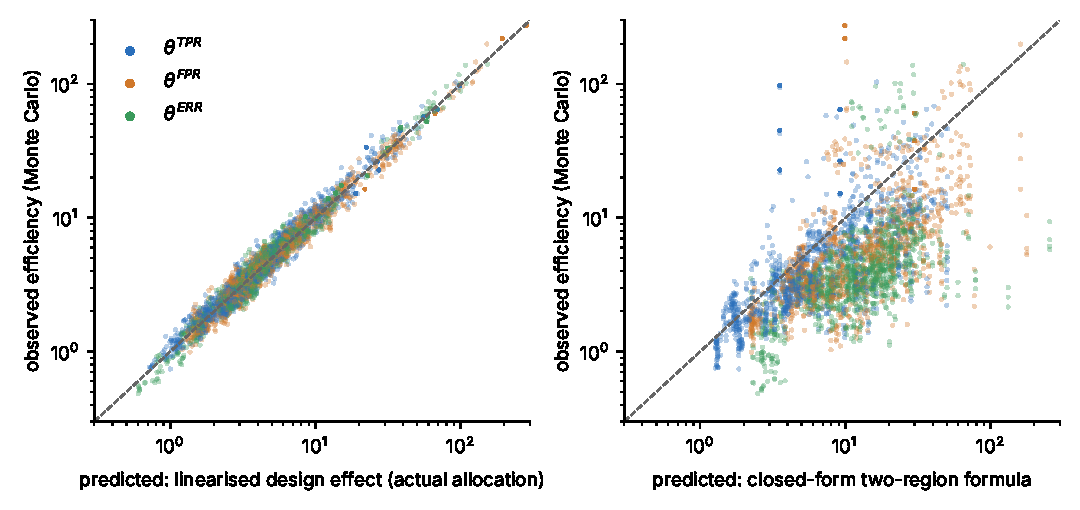
\includegraphics[width=\textwidth]{fig_sim_real}
\caption{Real pools, all budgets: observed efficiency of PATTERN relative to SRS for each of the
3519 compared target--budget pairs against the linearised prediction LIN (left) and the closed-form
two-region formula FORM (right). Dashed: equality. Source: \texttt{results/theory\_check.json}.}
\label{fig:sim-real}
\end{figure*}

\paragraph{The linearised design effect is accurate.} Over the 3519 pairs the ratio of observed to
predicted efficiency has median 0.998 and 10\%--90\% range 0.83--1.22; 77\% of the ratios are within
20\% and 99\% within a factor 1.5, and the correlation of the logarithms is 0.988
(Figure~\ref{fig:sim-real}, left). The spread is what Monte Carlo error alone produces: each MSE is
an average of 200 squared errors, with a relative standard error of about $\sqrt{2/200}=0.10$ for
approximately normal errors, so the ratio of two independent MSEs has a relative standard error of
about 0.14 and a 10\%--90\% range of roughly 0.84--1.20. The medians per pool and budget agree as
well: the ratio of the observed median efficiency to the median LIN prediction lies between 0.88 and
1.20 for the 34 pool--budget combinations, and for each type of estimand separately the median of
these ratios is 0.99 (TPR), 0.98 (FPR) and 1.00 (error). The agreement includes the cases with very
large gains: for Churn at $L=500$ the observed efficiency of 32.4 (predicted 32.2) arises because
the disagreement strata are fully enumerated, which only the finite-population corrections in LIN
capture. The lower correlations for Electricity, Phoneme and MAGIC reflect the narrow range of
efficiencies across targets in those pools (most lie between 2 and 4), not a larger error. We
conclude that, for the purpose of predicting efficiency, the linearised variance of
Section~\ref{sec:theory-asym} is adequate already at $L=250$.

\paragraph{The closed form overstates the gain on real pools.} FORM is a much poorer predictor: the
median ratio of observed efficiency to FORM is 0.47 (10\%--90\%: 0.17--1.17), and the rule of thumb
$1/\rho$ is more optimistic still (Table~\ref{tab:sim-real}). The reason is the one anticipated in
Section~\ref{sec:theory-deff}: with nine models the strata $(G,K)$ do not isolate the disagreements of
a particular pair. The share of the pool on which some model disagrees, $\rho_{\rm any}$, is between
0.18 and 0.73, while the median pairwise rate is between 0.001 and 0.33, and by
\eqref{eq:deff-sandwich} the attainable gain lies between $1/\rho_{\rm any}$ and $1/\rho$. OWN, which
uses the actual strata, is much closer (median ratio of observed to OWN 0.87): the remaining 13\% is
the price of serving all 108 estimands with one allocation, which Proposition~\ref{prop:allocation}(d)
makes explicit. Law school is a degenerate case for FORM, since the median pair disagrees on 0.1\% of
the pool and many targets have nearly zero variance; FORM and the observed efficiencies are
negatively correlated there. FORM is therefore useful as an explanation of where the gain comes from
and as an upper guide for a pair-specific design, but not as a numerical prediction for the
nine-model design; for prediction, LIN should be used, and it requires nothing beyond the pool and a
pilot or proxy estimate of the stratum variances.

\subsection{Synthetic pools with a controlled disagreement rate}\label{sec:sim-synth}

To test the closed form where its assumptions hold, and to vary $\rho$ over a wide range, we
generated pools of $N=200\,000$ with two groups ($\zeta_1=0.3$, $p_0=0.30$, $p_1=0.20$). A share
$\rho\in\{1,2,5,10,20,40\}\%$ of instances is placed in a disagreement region. Outside it, all models
predict the same label, equal to $Y$ with probability 0.85. Inside it, with two models, model 1 is
right with probability $q_g$ and model 2 predicts the opposite label; we use $q=(0.65,0.35)$
(moderate group-wise gaps) and $q=(0.95,0.05)$ (large gaps, one-sided disagreements). With five
models, each model is right independently with a model- and group-specific probability between 0.40
and 0.70, conditionally on not all models agreeing. Each model's probability is
$\mathrm{logit}^{-1}\{1.73(2\hat y-1)+\varepsilon\}$ with $\varepsilon\sim N(0,1)$, and the proxy is their
average, as in the real pools. The budget is $L=1000$ and $R=1000$, so the Monte Carlo relative
standard error of an efficiency is about 0.06. With two models, the pattern strata separate agreement
from disagreement exactly, and we also ran, for each target, its own Neyman allocation computed from
the true stratum variances, which is the design FORM describes.

\begin{table*}[t]
\centering
\caption{Synthetic pools: observed (Obs), linearised (LIN) and closed-form (FORM) efficiency of
PATTERN relative to SRS for $\theta^{TPR}$ and $\theta^{ERR}$ (median over pairs for five models),
as a function of the disagreement rate $\rho$ ($N=200\,000$, $L=1000$, $R=1000$). Source:
\texttt{results/theory\_check.json}.}
\label{tab:sim-syn}
\setlength{\tabcolsep}{3pt}
\resizebox{\textwidth}{!}{%
\begin{tabular}{l rrr rrr @{\hskip 8pt} rrr rrr @{\hskip 8pt} rrr rrr}
\toprule
 & \multicolumn{6}{c}{Two models, moderate gaps} & \multicolumn{6}{c}{Two models, large gaps} & \multicolumn{6}{c}{Five models}\\
 \cmidrule(lr){2-7}\cmidrule(lr){8-13}\cmidrule(lr){14-19}
 & \multicolumn{3}{c}{$\theta^{TPR}$} & \multicolumn{3}{c}{$\theta^{ERR}$} & \multicolumn{3}{c}{$\theta^{TPR}$} & \multicolumn{3}{c}{$\theta^{ERR}$} & \multicolumn{3}{c}{$\theta^{TPR}$} & \multicolumn{3}{c}{$\theta^{ERR}$}\\
$\rho$ & Obs & LIN & FORM & Obs & LIN & FORM & Obs & LIN & FORM & Obs & LIN & FORM & Obs & LIN & FORM & Obs & LIN & FORM\\
\midrule
1\% & 190.3 & 216.0 & 102.2 & 174.1 & 181.1 & 115.5 & 56.2 & 55.8 & 46.2 & 665.4 & 608.0 & 517.0 & 172.9 & 198.3 & 170.7 & 158.1 & 162.9 & 203.2 \\
2\% & 54.3 & 57.4 & 43.7 & 56.7 & 58.2 & 55.7 & 22.2 & 26.0 & 23.4 & 251.5 & 240.7 & 261.2 & 44.9 & 64.2 & 82.9 & 49.8 & 55.3 & 99.7 \\
5\% & 14.9 & 18.6 & 16.6 & 23.2 & 20.2 & 22.1 & 10.0 & 9.7 & 9.5 & 88.1 & 83.1 & 103.7 & 17.4 & 21.0 & 32.9 & 19.5 & 19.6 & 40.1 \\
10\% & 7.2 & 8.9 & 8.4 & 8.6 & 9.6 & 10.9 & 4.4 & 5.1 & 5.1 & 45.6 & 42.5 & 53.5 & 9.2 & 11.0 & 17.5 & 8.9 & 9.4 & 20.1 \\
20\% & 4.4 & 4.7 & 4.6 & 5.0 & 4.8 & 5.5 & 2.4 & 2.8 & 2.8 & 16.7 & 20.3 & 25.6 & 4.9 & 5.4 & 9.0 & 4.7 & 4.6 & 10.0 \\
40\% & 2.3 & 2.5 & 2.5 & 2.4 & 2.4 & 2.7 & 1.7 & 1.6 & 1.8 & 9.5 & 10.1 & 12.4 & 2.5 & 2.8 & 4.7 & 2.3 & 2.3 & 5.0 \\
\bottomrule
\end{tabular}}
\end{table*}

\begin{figure*}[t]
\centering
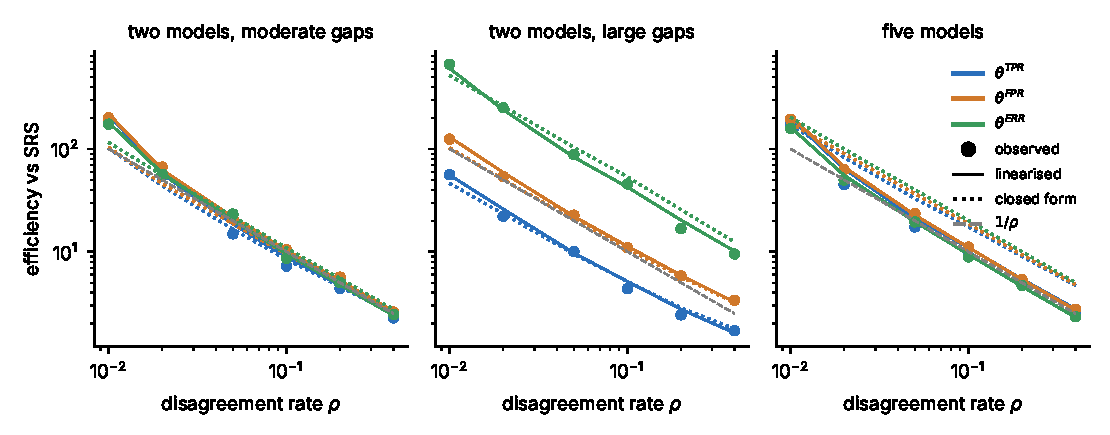
\includegraphics[width=\textwidth]{fig_sim_rho}
\caption{Synthetic pools: efficiency of PATTERN relative to SRS against the disagreement rate
$\rho$ (share of the pool in the disagreement region), median over pairs for each type of estimand.
Points: Monte Carlo ($R=1000$); solid: linearised prediction LIN; dotted: closed form FORM;
grey dashed: $1/\rho$. Source: \texttt{results/theory\_check.json}.}
\label{fig:sim-rho}
\end{figure*}

\paragraph{Efficiency scales as $1/\rho$.} In all three families the efficiency falls in proportion
to $1/\rho$ over a forty-fold range of $\rho$ (Figure~\ref{fig:sim-rho}). With two models and
moderate gaps, $\rho$ times the median observed efficiency is between 0.86 and 1.13 for
$\rho\ge2\%$, so the rule of thumb is accurate to about 15\%; at $\rho=1\%$ it is 1.9, because the
budget of 1000 labels is then about half the size of the disagreement region and the
finite-population correction roughly doubles the gain. LIN agrees with the observed efficiencies
throughout (median ratio per scenario between 0.88 and 1.04), with a tendency to be optimistic by a
few per cent that we attribute to the second-order terms neglected by the linearisation.

\paragraph{The closed form is accurate, and conservative, when its assumptions hold.} With two
models, the observed efficiency of the own-target Neyman design divided by FORM is between 0.90 and
1.25 for moderate gaps and $\rho\ge5\%$, and between 0.95 and 1.47 for large gaps; the LIN
predictions for the same designs give the same ratios, so the discrepancy is in the closed form and
not in the simulation. FORM is below the truth for two reasons stated in
Corollary~\ref{prop:deff}(a): it treats the agreement region as one stratum, whereas the pattern
design splits it by the common prediction ($K=0$ versus $K=M$, which have very different positive
rates), and it ignores the finite-population correction, which matters when the disagreement region
is small (at $\rho=1\%$ the ratio is 1.5 to 2.5). The large-gap family also shows the role of the
target size in Corollary~\ref{prop:deff}(c): the TPR gaps are large and the disagreements one-sided
($|a_g|=0.9$), and the gain for $\theta^{TPR}$ is only 0.45 to 0.7 times $1/\rho$, in line with
the factor $(\beta+\lambda)^{-2}$, which is about 0.4 for group 0 ($\pi_{\mathcal D}\approx
\pi_{\mathcal A}\approx0.3$) before the group factor $\Gamma$ is applied, while for the error difference, whose disagreements are nearly
deterministic within each group ($|\mu_g|=0.9$), the gain is several times $1/\rho$, as
\eqref{eq:deff-err} predicts.

\paragraph{With more models, the relevant rate is between $\rho_{\rm any}$ and the pairwise rate.} In
the five-model family the pairwise disagreement rate is about half of $\rho$, and FORM, which assumes
that each pair's disagreements are isolated, overstates the gain by a factor of about 1.9 (median
ratio of observed to FORM between 0.53 and 0.56 for $\rho\ge2\%$). The observed efficiency is instead
close to $1/\rho_{\rm any}$ ($\rho_{\rm any}$ times the median efficiency is between 0.94 and 1.06 for
$\rho\ge2\%$), the lower end of \eqref{eq:deff-sandwich}. This is expected: in this family the models
err independently inside the disagreement region, so a pair's disagreements are spread evenly over
the values of $K$. In the real pools, where models make correlated errors, the median OWN efficiency
lies inside the interval $[1/\rho_{\rm any},1/\rho]$ for every pool (Table~\ref{tab:sim-real}),
mostly in its lower half.

\subsection{Misspecified proxy}\label{sec:sim-proxy}

Proposition~\ref{prop:proxy} bounds the loss from a wrong proxy by the ratio \eqref{eq:proxy-loss}.
We took the five-model pool with $\rho=5\%$ and compared allocations computed from the default proxy,
from the true labels (oracle), from a constant proxy equal to the overall positive rate
(uninformative), from one minus the default proxy (inverted), and from an adversarial proxy that sets
$\pi_i=0.5$ where all models agree and $\pi_i=0.001$ where they do not, with proportional allocation
on the same strata as a reference.

\begin{table*}[t]
\centering
\caption{Proxy misspecification (five models, $\rho=5\%$, $L=1000$, $R=1000$). Loss: weighted
variance $\sum_tw_tV_t$ relative to the oracle allocation, predicted by the linearisation (pred.) and
observed with MSEs (obs.). Eff: harmonic mean over the 30 estimands of the efficiency relative to
SRS, predicted and observed, and the smallest observed efficiency. Kant.: Kantorovich bound of
Proposition~\ref{prop:proxy}(c) evaluated with the actual allocation. Source:
\texttt{results/theory\_check.json}.}
\label{tab:sim-proxy}
\small
\begin{tabular}{lrrrrrr}
\toprule
Allocation & Loss pred. & Loss obs. & Eff pred. & Eff obs. & min Eff obs. & Kant.\\
\midrule
Default proxy & 1.00 & 1.01 & 22.0 & 20.5 & 15.4 & 1.24\\
Oracle & 1.00 & 1.00 & 21.9 & 20.6 & 17.1 & 1.07\\
Uninformative & 1.00 & 1.01 & 21.9 & 20.5 & 16.6 & 1.23\\
Inverted & 1.00 & 0.98 & 22.0 & 21.2 & 17.2 & 1.24\\
Adversarial & 1.00 & 0.98 & 21.9 & 21.0 & 15.9 & 1.21\\
Proportional & 8.48 & 7.85 & 2.6 & 2.6 & 2.1 & 56.21\\
\bottomrule
\end{tabular}
\end{table*}

None of the four wrong proxies costs a measurable amount of efficiency (Table~\ref{tab:sim-proxy}):
the predicted loss is at most 0.2\%, the observed differences (between $-2.4\%$ and $+1.2\%$) are
within Monte Carlo error, and every one of the 30 estimands is estimated at least 15 times more
efficiently than under SRS. Proportional allocation on the same strata, by contrast, has eight times
the weighted variance. The explanation is Proposition~\ref{prop:influence}: the proxy enters the
anticipated stratum variances only through label rates, while the dominant feature, namely that the
comparison estimands receive almost no variance from the strata where all models agree, is fixed by
the predictions. With a constant or adversarial proxy the agreement strata are still anticipated to
have variance of order $\delta_g^2$, which is small, and the disagreement strata still have variance
of order one because $D_i$ varies within them; so all these allocations put almost the whole budget
into the disagreement strata and differ only in how it is divided among them. The Kantorovich bounds
(1.21--1.24) are valid but loose here. This robustness is specific to the structure of the problem
and should not be read as a general guarantee: Proposition~\ref{prop:proxy}(d) shows that a proxy
that misjudges a high-variance stratum can do arbitrarily badly in other stratified problems, and the
empirical comparison with the oracle allocation in Section~\ref{sec:ablations} is the relevant check
for real data.

\subsection{The difference estimator (PATTERN-DIF)}\label{sec:sim-dif}

Section~\ref{sec:theory-dif} makes four predictions about the difference estimator \eqref{eq:dif} with the proxy mean \eqref{eq:psi}: it is exactly unbiased for the totals
for any proxy and its plug-in variance is unbiased (Proposition~\ref{prop:validity}); its linearised variance is $V_\psi=\sum_hc_hS^2_{e,h}$ with residual influence values
$e_i=z_i-\tilde z_i$; its gain over the plain estimator on the same sample is $V_0/V_\psi$, which a label-free calculation forecasts under calibration
(Proposition~\ref{prop:dif-deff}); and a miscalibrated proxy can lose to the plain estimator (Proposition~\ref{prop:dif-proxy}). We check them with
\texttt{experiments/theory\_check\_dif.py} (results in \texttt{results/theory\_check\_dif.json}). Every comparison is between the plain and the
difference estimator on the \emph{same} PATTERN sample, so the ratio $\mathrm{MSE}(\text{plain})/\mathrm{MSE}(\text{DIF})$ isolates the estimator. Three predictions are used:
\textbf{LIN}, $\sum_hc_hS^2_{z,h}/\sum_hc_hS^2_{e,h}$, computed with the true labels; \textbf{ANT}, the label-free forecast
$\sum_hc_h(\bar\sigma^2_h+S^2_{\tilde z,h})/\sum_hc_h\bar\sigma^2_h$ of \eqref{eq:dif-deff}, which uses the proxy only; and \textbf{TUNE}, $V_\psi/V(\lambda)$ with $\lambda_h=\min\{1,\max(0,\beta_h)\}$, the
most that tuning the coefficient could add to $\lambda=1$.

\paragraph{Exactness and the variance formulae.} On a pool of 14 units in two strata (6 and 8 units, 2 and 3 labels) we enumerated all 840 samples for three proxies (a random mixture of $u_i,v_i$, an arbitrary bounded vector, and
the anti-correlated vector $1-t_i$) and three coefficients ($\lambda=0,\frac12,1$). The mean of $\hat T_{\lambda\psi}$, its covariance matrix and the mean of the plug-in variance estimator agree with $T$,
the formula of Proposition~\ref{prop:validity}(a) and each other to within $3\times10^{-13}$ in absolute terms (relative to the variances, $10^{-14}$), that is machine precision, for every proxy. By Monte Carlo ($R=2000$) the totals are also unbiased on the four real pools and six synthetic pools: the largest standardised bias
over the 29--49 coordinates is $|z|=2.7$ for the difference estimator and 2.6 for the plain estimator, which share their samples and have strongly correlated coordinates, and the largest bias is 0.06 standard deviations
(the Monte Carlo resolution is 0.022). The variance formula holds: the median over estimands of the Monte Carlo variance divided by the linearised $V_\psi$ is between 0.99 and 1.02 on the real pools (Table~\ref{tab:sim-dif-real}) and 1.01 to 1.07 on the synthetic
pools (up to 1.10 for $\theta^{TPR}$, a second-order effect of the random denominators at $L=600$), the mean of $\hat V_\psi$ divided by the Monte Carlo variance is between 0.98 and 1.02, and the Wald coverage of the difference estimator
(0.943 to 0.951 on the real pools, 0.947 to 0.953 on the synthetic pools) is that of the plain estimator.

\begin{table*}[t]
\centering
\caption{Four real pools, $R=2000$: efficiency of the difference estimator relative to the plain estimator on the same PATTERN sample (median over the 108 estimands). Obs: Monte Carlo; LIN, ANT, TUNE:
predictions defined in the text; Obs/LIN: per-target ratio, median and 10\%--90\% range, and correlation of the logarithms; Var: Monte Carlo variance of $\hat\theta_{\rm DIF}$ over $V_\psi$; $\hat V$: mean estimated over Monte Carlo variance; Cov: Wald coverage of plain
and difference estimator; max $|z|$: largest standardised bias of the 46--49 totals. Source: \texttt{results/theory\_check\_dif.json}.}
\label{tab:sim-dif-real}
\small
\resizebox{\textwidth}{!}{%
\begin{tabular}{lrrrrrlrrrrrr}
\toprule
Pool & $L$ & Obs & LIN & ANT & TUNE & Obs/LIN & corr & Var & $\hat V$ & Cov plain & Cov DIF & max $|z|$\\
\midrule
Adult-sex & 500 & 1.50 & 1.46 & 1.47 & 1.01 & 1.01 (0.99, 1.04) & 0.998 & 0.99 & 1.02 & 0.949 & 0.951 & 1.6\\
Bank & 500 & 1.45 & 1.48 & 1.46 & 1.01 & 0.99 (0.96, 1.03) & 0.994 & 1.02 & 0.99 & 0.942 & 0.943 & 2.0\\
EEG & 500 & 1.90 & 1.91 & 1.43 & 1.04 & 1.00 (0.97, 1.03) & 0.997 & 1.00 & 1.00 & 0.947 & 0.948 & 2.2\\
Spambase & 250 & 2.30 & 2.34 & 1.97 & 1.02 & 1.00 (0.96, 1.03) & 0.998 & 1.00 & 0.99 & 0.944 & 0.945 & 1.4\\
\bottomrule
\end{tabular}}
\end{table*}

\begin{figure*}[t]
\centering
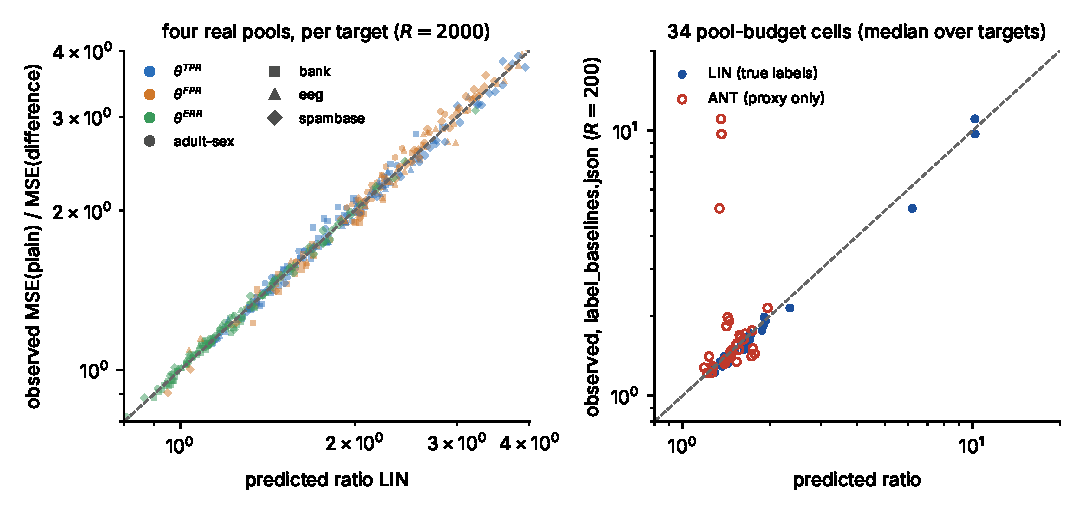
\includegraphics[width=\textwidth]{fig_sim_dif_real}
\caption{Left: observed against linearised (LIN) gain of the difference estimator over the plain estimator, per estimand, on four real pools ($R=2000$; 432 estimands). Right: median over estimands in each of 34 pool--budget
cells, observed in \texttt{results/label\_baselines.json} (PATTERN-DIF against PATTERN, $R=200$) against LIN (filled) and ANT (open). Dashed: equality. Source: \texttt{results/theory\_check\_dif.json}.}
\label{fig:sim-dif-real}
\end{figure*}

\paragraph{Predicted against observed gain.} On the four real pools the observed per-estimand gain divided by LIN has median 1.00 and 10\%--90\% range 0.97--1.04 (432 estimands, correlation of the logarithms 0.997; Figure~\ref{fig:sim-dif-real}, left), which
is Monte Carlo error. We then compared LIN with the gains stored in \texttt{results/label\_baselines.json}, which were produced independently by \texttt{experiments/label\_baselines.py} with $R=200$. In the 34 cells with a defined gain (all 35 except Law school at
$L=2000$, where both estimators are exact) the observed median gain is 1.47 (10\%--90\% range 1.28--2.10, extremes 1.22 and 11.1), LIN has median 1.49, and the ratio of observed to LIN has median 0.98 (10\%--90\% range 0.93--1.01, 97\% of cells within 20\%, correlation of the logarithms 0.996, 0.978 without
the three Law school cells); Figure~\ref{fig:sim-dif-real} (right). LIN uses the labels, so it is not a forecast, but it confirms that the residual-variance formula $V_\psi$ describes the estimator. The label-free forecast
ANT has median ratio 1.01 (0.90--1.37) over cells, and on the four real pools ratio 1.12 (0.86--1.53) with correlation 0.78 across estimands; the observed gain is 1.30 and 1.37 times ANT in EEG and Spambase. It fails in Law school (forecast 1.3--1.4, observed 5.1--11.1), where the
disagreement sets of most pairs contain a handful of units per stratum: the realised residual variance is then a single draw from the label distribution, and it is an order of magnitude below its expectation under the proxy (we checked the stratum variances for one estimand). Without Law school the correlation of ANT with the observed gain is 0.62.
The gain is therefore not a doubling in general: it is 1.2 to 1.7 in most cells, about 1.8 to 2.1 in EEG and Spambase, and 5 to 11 only in Law school. By estimand type the order is that of \eqref{eq:dif-closed}: the gain is largest for $\theta^{FPR}$,
next for $\theta^{TPR}$ and smallest for $\theta^{ERR}$ (Adult-sex: 2.25, 1.67 and 1.13; Table~\ref{tab:sim-dif-syn} for the synthetic pools).

\paragraph{Tuning the coefficient.} TUNE is small: the median over the 34 cells is 1.02 (10\%--90\% 1.01--1.04), and 1.01 to 1.04 on the four real pools, so a perfectly tuned coefficient would add at most a few per cent to $\lambda=1$ except in Law school (2.3--3.5).
The observed estimated-coefficient version (PATTERN-PPI) has median gain 1.03 over $\lambda=1$ (10\%--90\% 0.99--1.10), and it costs coverage: mean coverage over the 35 cells is 0.946 for PATTERN-DIF and 0.929 for PATTERN-PPI, and 8 of 35 cells fall below 0.93 for PATTERN-PPI against 1 of 35 for PATTERN-DIF
and for the plain estimator. This is the trade-off of Proposition~\ref{prop:dif-lambda}.

\paragraph{Allocation.} The residual-variance allocation of Proposition~\ref{prop:alloc-dif} does not improve on the design's plain-variance allocation for the difference estimator. The linearised prediction of the ratio of $V_\psi$ under the plain allocation to $V_\psi$ under the residual allocation has median 0.99
(10\%--90\% 0.95--1.00) over the 34 cells, and on four real pools the observed ratio of mean squared errors is 0.98, 0.98, 0.98 and 1.01, against linearised predictions 1.00, 1.00, 0.98 and 1.00, with the same coverage. Using the ``wrong'' variances therefore costs at most about 2\% here, as the bound \eqref{eq:alloc-loss} allows when the signal-to-noise ratio $\tilde\nu_h$ is similar across strata.

\begin{table*}[t]
\centering
\caption{Synthetic pools ($N=60\,000$, five models, $Y_i\sim$ Bernoulli$(\pi_i)$, $L=600$, $R=2000$): gain of the difference estimator over the plain estimator, observed (Obs), linearised (LIN) and label-free (ANT), median over the ten pairs. Top: calibrated proxy,
sharpness $a$ of the latent score. Bottom: $a=2$, proxy $\pi^{\rm proxy}_i=\mathrm{logit}^{-1}(\kappa s_i)$ ($\kappa=1$ calibrated, $\kappa=0$ constant 0.5, $\kappa<0$ inverted). Source: \texttt{results/theory\_check\_dif.json}.}
\label{tab:sim-dif-syn}
\setlength{\tabcolsep}{4pt}
\small
\begin{tabular}{l rrr rrr rrr}
\toprule
 & \multicolumn{3}{c}{$\theta^{TPR}$} & \multicolumn{3}{c}{$\theta^{FPR}$} & \multicolumn{3}{c}{$\theta^{ERR}$}\\
 \cmidrule(lr){2-4}\cmidrule(lr){5-7}\cmidrule(lr){8-10}
 & Obs & LIN & ANT & Obs & LIN & ANT & Obs & LIN & ANT\\
\midrule
$a=0.5$ & 1.76 & 1.76 & 1.76 & 2.40 & 2.44 & 2.47 & 1.10 & 1.09 & 1.10 \\
$a=1$ & 2.03 & 1.97 & 1.98 & 2.33 & 2.33 & 2.36 & 1.09 & 1.09 & 1.10 \\
$a=2$ & 2.11 & 2.12 & 2.14 & 2.21 & 2.32 & 2.31 & 1.11 & 1.12 & 1.11 \\
$a=4$ & 2.23 & 2.23 & 2.24 & 2.26 & 2.27 & 2.26 & 1.11 & 1.12 & 1.12 \\
\midrule
$\kappa=-1$ & 1.43 & 1.48 & 2.29 & 1.52 & 1.56 & 2.15 & 0.76 & 0.76 & 1.12 \\
$\kappa=0$ & 1.88 & 1.94 & 2.00 & 2.04 & 2.05 & 2.00 & 1.00 & 1.00 & 1.00 \\
$\kappa=0.5$ & 2.11 & 2.11 & 2.02 & 2.23 & 2.22 & 2.09 & 1.10 & 1.09 & 1.03 \\
$\kappa=1$ & 2.21 & 2.16 & 2.15 & 2.28 & 2.27 & 2.29 & 1.12 & 1.12 & 1.12 \\
$\kappa=2$ & 2.09 & 2.06 & 2.59 & 2.22 & 2.17 & 2.89 & 1.08 & 1.07 & 1.39 \\
$\kappa=4$ & 1.81 & 1.80 & 3.81 & 1.89 & 1.90 & 4.45 & 0.96 & 0.94 & 2.11 \\
\bottomrule
\end{tabular}
\end{table*}

\begin{figure*}[t]
\centering
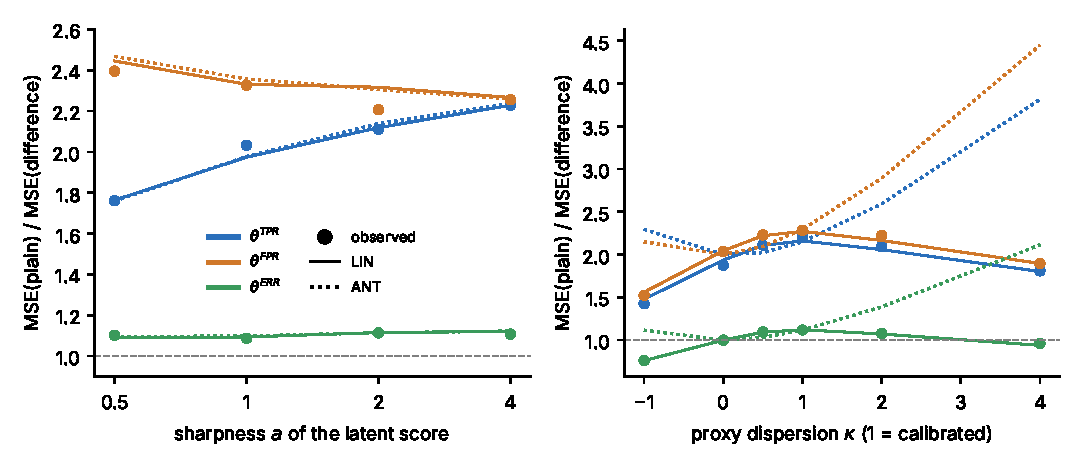
\includegraphics[width=\textwidth]{fig_sim_dif_synth}
\caption{Synthetic pools, gain of the difference estimator over the plain estimator (median over pairs, by estimand). Left: calibrated proxy, sharpness $a$ of the latent score. Right: $a=2$, proxy dispersion $\kappa$ ($\kappa=1$ calibrated).
Points: Monte Carlo ($R=2000$); solid: LIN; dotted: ANT, which assumes calibration. Dashed: no gain. Source: \texttt{results/theory\_check\_dif.json}.}
\label{fig:sim-dif-synth}
\end{figure*}

\paragraph{Calibrated and miscalibrated proxies.} In pools whose labels follow the proxy, ANT and LIN agree with each other and with the Monte Carlo gain within 2\% (median observed/LIN between 0.99 and 1.00; Table~\ref{tab:sim-dif-syn}, top), which verifies
Proposition~\ref{prop:dif-deff}: the gain is 1.8 to 2.4 for the rate differences and 1.1 for the error difference, because in the disagreement strata the proxy is uncertain ($\overline{\pi(1-\pi)}$ is large) and the closed forms \eqref{eq:dif-closed} are bounded; a sharper latent score hardly changes them. For miscalibrated proxies
(bottom), unbiasedness and coverage are unaffected (coverage 0.947--0.953), LIN keeps tracking the Monte Carlo gain (median ratio 0.99 to 1.01) and ANT, which assumes calibration, does not. The theory's two warnings appear. First, an inverted proxy ($\kappa=-1$) makes the difference estimator \emph{worse} than the plain estimator for the error difference
(gain 0.76, that is 1.3 times the mean squared error, as LIN predicts), while the rate differences still gain 1.4 to 1.5. The design-weighted slope $\bar\beta=\sum_hc_h\mathrm{Cov}_h(z,\tilde z)/\sum_hc_hS^2_{\tilde z,h}$ of the error difference is $-1.02$, the clipped coefficient is $0$ and TUNE, which here recovers the plain estimator, is 1.32 $=1/0.76$. Second, a constant proxy $\pi_i\equiv\frac12$ ($\kappa=0$) is uninformative for the error difference (gain exactly 1, since $\tilde z\equiv0$) but not for the
rate differences (1.9 and 2.0, TUNE 1.03 and 1.04), because $\tilde z_i$ still carries the known pattern of $D_i$. Third, the threshold $\beta<\frac12$ of Proposition~\ref{prop:dif-var}(a) is visible: for the error difference $\bar\beta$ is 1.02 at $\kappa=1$, 0.62 at $\kappa=2$ (gain 1.08) and 0.44 at $\kappa=4$ (gain 0.96), so an over-sharp proxy gains little for the rate differences (1.8--1.9) and crosses to a loss for the error difference.

\paragraph{Zero-variance strata and the floor.} The residual floor \eqref{eq:floor} was evaluated on four pools at $L=250$ ($R=1000$). At Churn the difference estimator alone raises the worst-estimand coverage from 0.52 (plain estimator, \texttt{results/label\_baselines.json}) to 0.84 (0.87 in this run), because
$\hat e_i=-\pi_i\hat d_i$ varies even when no positive is sampled; at Law school it does not (0.64 for both). Where the problem persists the floor repairs it: for Law school mean coverage rises from 0.913 to 0.954 and the worst-estimand coverage from 0.65 to 0.89; for Adult-sex and Credit card default the mean rises from 0.942 to 0.946 and from 0.949 to 0.955 with the worst estimand unchanged (0.85 and 0.92); at Churn the floor is active in 0.2\% of
(replication, estimand) pairs and changes nothing (0.938). The floor widens the intervals by a median factor of 1.00 (90th percentile 1.08, 1.15, 1.33 for Adult-sex, Credit card and Law school). It does not alter the point estimate. As in Section~\ref{sec:ablations} it is a safeguard chosen after seeing the failure, and these numbers are not an out-of-sample test.

\subsection{Summary}

The linearised design effect predicts the efficiency of the implemented design to within Monte
Carlo error on all 11 real pools and in the synthetic families (per-target median ratio 1.00,
10\%--90\% range 0.83--1.22 on the real pools). The closed form of Corollary~\ref{prop:deff} is
accurate and conservative when the strata separate a pair's agreements from its disagreements (the
own-target efficiency is 0.90 to 1.47 times the formula for $\rho\ge5\%$), and it captures the $1/\rho$ scaling and the effect of the
target size. With nine models it overstates the gain on real pools by a median factor of about two,
because the counts $K$ locate any disagreement but not that of a specific pair; the bounds
$1/\rho_{\rm any}\le\mathrm{Eff}\le1/\rho$ of \eqref{eq:deff-sandwich} describe this gap. The gain vanishes
only as the disagreement rate approaches one, as in EEG ($\rho_{\rm any}=0.73$, efficiency 1.6--1.9). For the difference estimator the linearised residual variance predicts the observed gain over the plain estimator within Monte Carlo error
(median ratio 0.98 over 34 pool--budget cells; Section~\ref{sec:sim-dif}), the label-free forecast does so except in Law school, and the gain is moderate (median 1.47) rather than a doubling.

\section{Empirical study on eleven data settings}\label{sec:empirical}

\subsection{Data, models and protocol}
We use eleven settings built from ten public binary classification data sets available on OpenML (Table~\ref{tab:data}; details in Appendix~\ref{app:data}). In five settings the group is a protected attribute: sex or race in Adult, age below 30 in Bank Marketing, sex in the credit-card default data and race in the law-school admission data. In the other six the group is an arbitrary split of the first numeric feature at its median, removed from the features; these settings have no fairness meaning but test the design on a wider range of prediction structures. A twelfth candidate (Nomao) was excluded because its arbitrary group contains no positive instances.

Each data set is split once into a training part (60\%) and a pool (40\%); the Electricity data (45,312 rows) were first subsampled to 30,000, while Adult and Bank Marketing are used in full. Nine classifiers are trained on the training part with scikit-learn: logistic regression with default and with strong regularisation, decision trees of depth 3 and 12, a random forest, histogram gradient boosting, 25-nearest neighbours, Gaussian naive Bayes and a multilayer perceptron. Their predictions and predicted probabilities on the pool, together with the group attribute, are all the design uses. The pool labels play two roles: they answer label queries, and they define the true values of the estimands, so that the error of every estimate is known exactly.

For each setting and budget $L\in\{250,500,1000,2000\}$ with $L\le N/4$ (35 setting--budget cells), we draw 200 independent labelled samples under each design and compute the $3\binom{9}{2}=108$ comparison estimands of \eqref{eq:theta}. The efficiency of a design is the ratio of the mean squared error under SRS to that under the design, computed for each estimand and summarised by the median over estimands; an efficiency of 4 means that SRS needs about four times as many labels to reach the same accuracy. Estimands whose true value is identically degenerate in the pool (for example when no model pair disagrees in a group) are excluded; this affects 51 of 108 estimands in the law-school setting only. Efficiencies are computed over the samples in which both designs give finite estimates; SRS produced an undefined estimate (no sampled positive in a group) in at most 0.5\% of its samples and the stratified designs never did. The designs are those of Section~\ref{sec:design}: SRS, SRS-DIF, GROUP, GROUP-DIF, PATTERN (plain estimator) and the proposed PATTERN-DIF, together with a variant of PATTERN-DIF whose allocation uses the residual variances. The first three designs are drawn exactly as in an earlier version of this study, so the SRS, GROUP and PATTERN samples coincide. The code and all results are in the repository (\texttt{experiments/label\_efficiency\_dif.py}, \texttt{results/label\_efficiency\_dif.json}).

\begin{table*}[t]\centering\footnotesize
\caption{Data settings. Pool: size of the held-out pool from which labels are drawn. $P_0,P_1$: positives in each group. Disagreement: share of pool instances on which two of the three most accurate models disagree, averaged over the three pairs. Groups marked ``arbitrary'' are median splits of a numeric feature.}\label{tab:data}
\begin{tabular}{lcrrrr}\toprule
Setting & Group & Pool $N$ & Positives $P_0$ & Positives $P_1$ & Disagreement \\\midrule
Adult (sex) & sex & 19537 & 3963 & 712 & 0.053 \\
Adult (race) & race & 19537 & 4249 & 426 & 0.047 \\
Bank marketing & age & 18085 & 1753 & 363 & 0.045 \\
Credit card & sex & 12000 & 1148 & 1506 & 0.030 \\
Law school & race & 8320 & 2038 & 640 & 0.000 \\
MAGIC & arbitrary & 7608 & 1084 & 1591 & 0.049 \\
EEG eye state & arbitrary & 5992 & 1183 & 1506 & 0.086 \\
Phoneme & arbitrary & 2162 & 388 & 247 & 0.095 \\
Spambase & arbitrary & 1841 & 490 & 235 & 0.043 \\
Churn & arbitrary & 2000 & 149 & 134 & 0.041 \\
Electricity & arbitrary & 12000 & 2582 & 2488 & 0.086 \\
\bottomrule\end{tabular}
\end{table*}

\subsection{Efficiency}
Table~\ref{tab:efficiency} gives the efficiency of every design in every cell, Table~\ref{tab:decomposition} summarises it by budget and Figure~\ref{fig:efficiency} shows it as a function of the budget and of the disagreement rate. Across settings, the median efficiency of PATTERN-DIF relative to SRS was 5.8 at $L=250$ (eleven settings), 6.3 at $L=500$ (ten), 6.9 at $L=1000$ (eight) and 15.5 at $L=2000$ (six); without the degenerate law-school setting the medians are 5.5, 5.8, 6.0 and 9.4. In other words, SRS needs between five and sixteen times as many labels to match the accuracy of PATTERN-DIF on the comparisons of interest, and the lowest efficiency in any cell outside law school was 3.5. The medians over settings rise with the budget partly because the set of settings changes (only the larger pools allow the larger budgets): on the seven non-degenerate settings that are present at $L=250$, 500 and 1000 the medians of PATTERN-DIF are 5.3, 5.3 and 6.0 (3.5, 3.8 and 4.4 for PATTERN). Within each of these seven settings the efficiency does increase with the budget (a median increase of 23\% from $L=250$ to $L=1000$), as larger budgets allow the design to label a larger share of the small disagreement strata, where the variance of the comparisons is concentrated; the increase is moderate except at $L=2000$, where the settings that remain are those with the largest pools and the strongest gains.

\paragraph{Where the gain comes from.} The decomposition in Table~\ref{tab:decomposition} separates the two ingredients. The design is the larger one. Under the difference estimator, moving from simple random sampling to the PATTERN strata multiplies the efficiency by 3.3 to 8.6 (PATTERN-DIF against SRS-DIF), and under the plain estimator by 3.7 to 7.3 (PATTERN against SRS). The estimator contributes 1.3 to 1.65 on top of the PATTERN design (PATTERN-DIF against PATTERN, better in 34 of 35 cells), but only 1.8 to 2.0 on top of simple random sampling (SRS-DIF against SRS). The design and the estimator are therefore complementary, and neither accounts for the whole gain. Stratifying by group alone gave no gain under the plain estimator (median 1.0 at every budget) and 2.1 to 2.7 with the difference estimator, which is essentially the value of the proxy correction: the variance of a contrast between two models is driven by the instances on which they disagree, and these are spread over both groups.

\paragraph{By estimand.} Efficiency differed by estimand. For PATTERN-DIF the medians over settings at the four budgets were 5.8, 5.3, 8.9 and 17.0 for $\theta^{\mathrm{TPR}}$, 7.6, 8.5, 8.4 and 20.6 for $\theta^{\mathrm{FPR}}$, and 3.5, 4.1, 4.4 and 5.7 for $\theta^{\mathrm{ERR}}$. The fairness contrasts gain more than the error contrast, because they depend on the rarest cells (positives or negatives in the minority group). In Adult with race as the group, at $L=1000$, the efficiencies were 23.9 for $\theta^{\mathrm{TPR}}$, 20.6 for $\theta^{\mathrm{FPR}}$ and 3.7 for $\theta^{\mathrm{ERR}}$. For the pairs formed by the three most accurate models, the comparisons a practitioner is most likely to care about, the median efficiency of PATTERN-DIF was 5.8, 6.8, 6.6 and 10.5 at the four budgets (3.3, 4.2, 3.9 and 6.2 for PATTERN).

\begin{figure*}[t]\centering
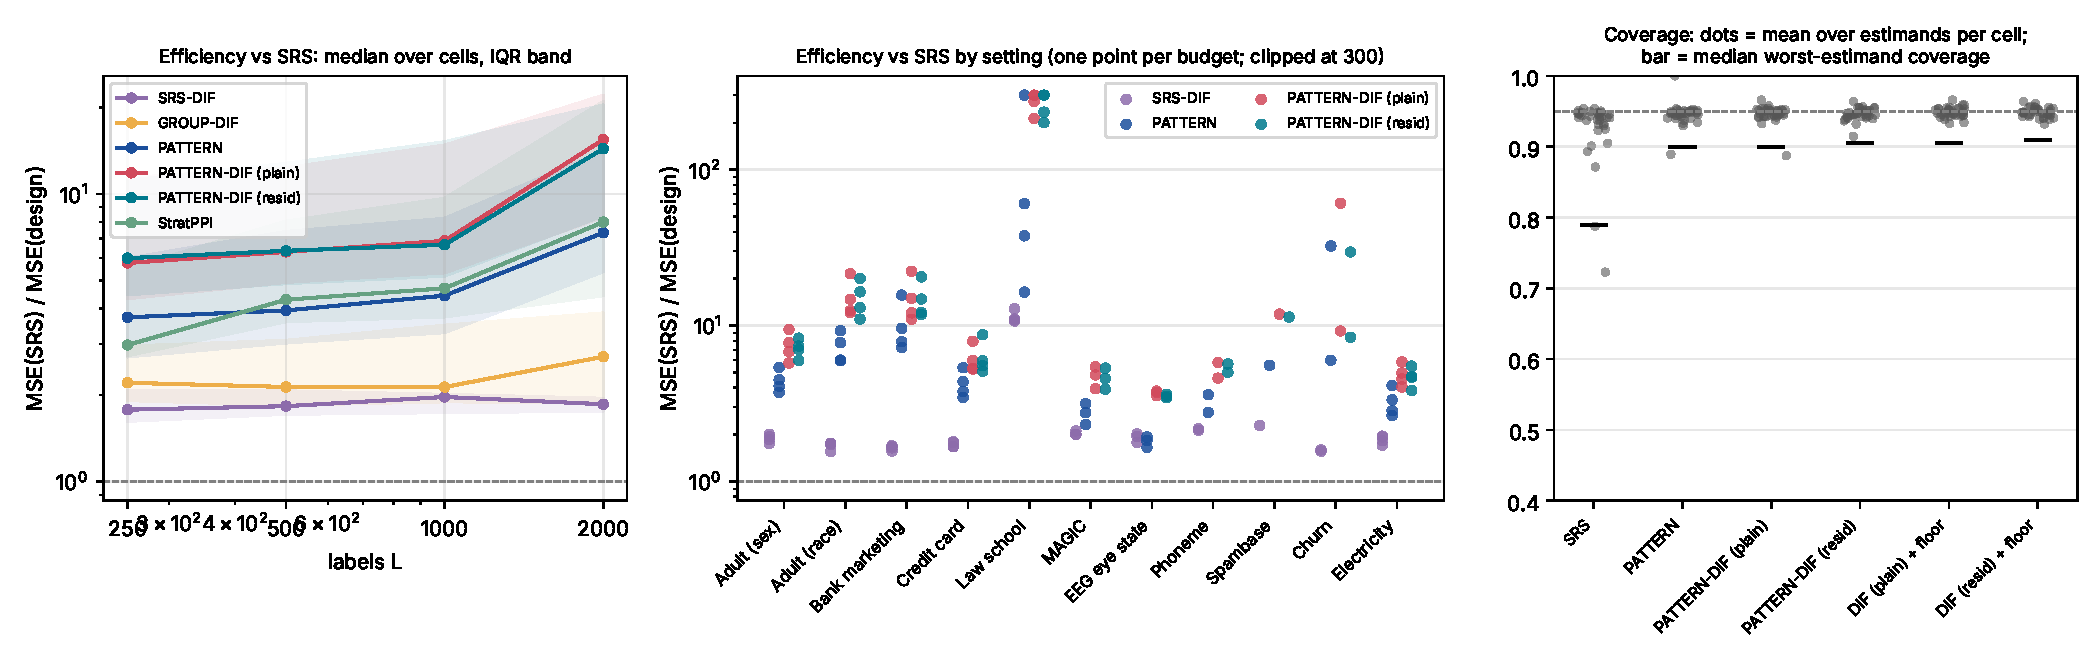
\includegraphics[width=\textwidth]{efficiency_dif}
\caption{Efficiency of the designs relative to SRS (median over the comparison estimands) as a function of the label budget and of the disagreement rate; see Table~\ref{tab:efficiency} for the numbers.}\label{fig:efficiency}
\end{figure*}

\begin{table*}[t]\centering\footnotesize
\caption{Decomposition of the efficiency gain by budget (median over settings of the cell medians). Each row is a ratio of mean squared errors. ``DIF resid vs DIF plain'' compares the residual-variance allocation with the allocation used by default.}\label{tab:decomposition}
\begin{tabular}{lrrrr}\toprule
Step (MSE ratio) & $L=250$ & $L=500$ & $L=1000$ & $L=2000$ \\\midrule
SRS-DIF vs SRS & 1.78 & 1.83 & 1.97 & 1.86 \\
PATTERN vs SRS & 3.72 & 3.94 & 4.43 & 7.33 \\
PATTERN-DIF vs PATTERN & 1.65 & 1.54 & 1.51 & 1.31 \\
PATTERN-DIF vs SRS-DIF & 3.28 & 3.29 & 3.72 & 8.57 \\
PATTERN-DIF vs SRS & 5.76 & 6.29 & 6.87 & 15.5 \\
DIF resid vs DIF plain & 1.01 & 0.97 & 0.96 & 1.00 \\
\bottomrule\end{tabular}

\end{table*}

\subsection{Efficiency and disagreement}
The gain is larger when the models disagree less (Figure~\ref{fig:efficiency}). The Spearman correlation between the disagreement rate of the three best models and the efficiency of PATTERN-DIF was $-0.58$ at $L=250$ (ten settings), $-0.53$ at $L=500$ (nine) and $-0.71$ at $L=1000$ (seven), excluding law school. The three settings with the highest disagreement (EEG, electricity and phoneme, 8.6\% to 9.5\%) had the smallest gains, between 3.7 and 5.8 at $L=500$. The relation is not exact, because efficiency also depends on the size of the minority cells and on the magnitude of the contrasts; Section~\ref{sec:theory} makes this precise and Section~\ref{sec:simulation} checks it.

Two settings are atypical. In the law-school data all nine models predict almost identically (the three best models disagree on fewer than 0.01\% of instances); the design then labels almost every disagreement instance and the contrasts are estimated nearly exactly, so the efficiency ratios (about 270 at $L=500$, 510 at $L=1000$ and above $10^{4}$ at $L=2000$) say little beyond the fact that SRS wastes labels on agreements. In the churn data (a pool of 2,000) the efficiency of PATTERN-DIF at $L=500$ was 61, driven by contrasts of false positive rates and of errors that are concentrated in very few instances.

\begin{table*}[p]\centering\footnotesize
\caption{Efficiency (ratio of mean squared errors, median over estimands) by setting and budget. DIF plain: PATTERN-DIF with the default allocation; DIF resid: with the residual-variance allocation; StratPPI: stratified prediction-powered inference (Section~\ref{sec:baselines}). ``vs PATTERN'': PATTERN-DIF relative to the plain estimator under the same design. The last three columns are the efficiencies of PATTERN-DIF by estimand type. Bold marks the best of the two PATTERN-DIF variants.}\label{tab:efficiency}
\begin{tabular}{lrrrrrrrr rrr}\toprule
Setting & $L$ & \multicolumn{6}{c}{Efficiency vs SRS} & vs PATTERN & \multicolumn{3}{c}{PATTERN-DIF (plain) by estimand} \\
 & & SRS-DIF & GROUP-DIF & PATTERN & DIF plain & DIF resid & StratPPI & DIF plain & $\theta^{TPR}$ & $\theta^{FPR}$ & $\theta^{ERR}$ \\\midrule
Adult (sex) & 250 & 1.75 & 2.20 & 3.72 & 5.76 & \textbf{5.98} & 3.28 & 1.37 & 8.68 & 7.59 & 3.50 \\
 & 500 & 1.86 & 1.95 & 4.08 & 6.80 & \textbf{7.02} & 4.07 & 1.49 & 9.30 & 8.20 & 3.83 \\
 & 1000 & 2.01 & 1.91 & 4.49 & \textbf{7.76} & 7.39 & 4.71 & 1.51 & 11.8 & 8.75 & 4.28 \\
 & 2000 & 1.94 & 1.87 & 5.39 & \textbf{9.42} & 8.30 & 5.54 & 1.32 & 11.7 & 11.8 & 5.03 \\
\addlinespace
Adult (race) & 250 & 1.56 & 3.31 & 5.96 & \textbf{12.1} & 11.0 & 5.46 & 1.65 & 18.1 & 15.4 & 2.96 \\
 & 500 & 1.73 & 3.33 & 6.02 & 12.4 & \textbf{13.0} & 6.95 & 1.44 & 17.5 & 14.9 & 3.44 \\
 & 1000 & 1.76 & 3.36 & 7.78 & 14.7 & \textbf{16.5} & 8.52 & 1.48 & 23.9 & 20.6 & 3.70 \\
 & 2000 & 1.75 & 3.52 & 9.28 & \textbf{21.5} & 20.0 & 10.4 & 1.30 & 37.5 & 29.3 & 4.36 \\
\addlinespace
Bank marketing & 250 & 1.57 & 3.84 & 7.22 & 11.0 & \textbf{11.8} & 7.80 & 1.44 & 11.0 & 18.6 & 5.05 \\
 & 500 & 1.64 & 3.99 & 7.87 & 12.1 & \textbf{12.1} & 10.3 & 1.45 & 12.1 & 24.7 & 6.31 \\
 & 1000 & 1.67 & 3.90 & 9.60 & \textbf{15.0} & 14.8 & 13.1 & 1.43 & 15.6 & 38.9 & 6.56 \\
 & 2000 & 1.69 & 3.97 & 15.7 & 22.3 & 20.5 & \textbf{24.5} & 1.32 & 22.3 & 79.9 & 9.18 \\
\addlinespace
Credit card & 250 & 1.67 & 1.86 & 3.45 & \textbf{5.31} & 5.09 & 2.58 & 1.26 & 3.55 & 7.18 & 4.27 \\
 & 500 & 1.80 & 1.81 & 3.79 & 5.26 & \textbf{5.53} & 3.52 & 1.29 & 4.81 & 7.84 & 4.30 \\
 & 1000 & 1.67 & 1.68 & 4.37 & \textbf{5.98} & 5.94 & 3.71 & 1.42 & 5.90 & 8.01 & 5.00 \\
 & 2000 & 1.78 & 1.91 & 5.36 & 7.93 & \textbf{8.72} & 4.06 & 1.20 & 5.43 & 10.5 & 6.32 \\
\addlinespace
Law school & 250 & 10.9 & 22.2 & 16.4 & \textbf{$>$100} & $>$100 & 31.8 & 10.7 & $>$100 & $>$100 & $>$100 \\
 & 500 & 12.8 & 19.7 & 37.6 & \textbf{$>$100} & $>$100 & 52.4 & 9.46 & $>$100 & $>$100 & $>$100 \\
 & 1000 & 11.0 & 21.4 & 60.4 & \textbf{$>$100} & $>$100 & 78.4 & 8.26 & $>$100 & $>$100 & $>$100 \\
 & 2000 & 10.7 & 20.4 & \textbf{$>$100} & $>$100 & $>$100 & $>$100 & 0.00 & $>$100 & $>$100 & $>$100 \\
\addlinespace
MAGIC & 250 & 2.01 & 1.98 & 2.32 & \textbf{3.93} & 3.90 & 2.71 & 1.65 & 3.89 & 5.30 & 3.06 \\
 & 500 & 2.11 & 2.26 & 2.76 & \textbf{4.82} & 4.57 & 3.81 & 1.71 & 4.89 & 5.94 & 3.27 \\
 & 1000 & 2.01 & 2.10 & 3.16 & \textbf{5.43} & 5.33 & 4.69 & 1.61 & 4.73 & 6.75 & 4.60 \\
\addlinespace
EEG eye state & 250 & 1.78 & 1.96 & 1.65 & \textbf{3.55} & 3.51 & 2.71 & 1.93 & 3.80 & 4.06 & 2.98 \\
 & 500 & 1.94 & 2.00 & 1.83 & \textbf{3.73} & 3.44 & 3.33 & 1.82 & 4.23 & 3.99 & 3.15 \\
 & 1000 & 2.02 & 2.16 & 1.93 & \textbf{3.80} & 3.61 & 3.68 & 1.91 & 4.06 & 4.86 & 3.04 \\
\addlinespace
Phoneme & 250 & 2.13 & 2.29 & 2.77 & 4.60 & \textbf{5.02} & 2.98 & 1.77 & 4.68 & 6.74 & 3.19 \\
 & 500 & 2.18 & 2.41 & 3.60 & \textbf{5.79} & 5.67 & 4.51 & 1.78 & 5.66 & 8.71 & 4.36 \\
\addlinespace
Spambase & 250 & 2.29 & 2.61 & 5.55 & \textbf{11.8} & 11.3 & 5.56 & 2.19 & 16.1 & 20.0 & 5.69 \\
\addlinespace
Churn & 250 & 1.56 & 1.49 & 5.99 & \textbf{9.22} & 8.41 & 2.96 & 1.42 & 5.77 & 10.3 & 9.48 \\
 & 500 & 1.59 & 1.78 & 32.4 & \textbf{60.8} & 29.6 & 8.42 & 1.28 & 4.46 & 70.6 & 77.1 \\
\addlinespace
Electricity & 250 & 1.83 & 1.84 & 2.65 & \textbf{4.04} & 3.83 & 2.76 & 1.63 & 4.88 & 5.26 & 2.97 \\
 & 500 & 1.71 & 1.78 & 2.84 & 4.54 & \textbf{4.66} & 3.40 & 1.59 & 4.82 & 5.42 & 3.20 \\
 & 1000 & 1.93 & 1.85 & 3.34 & \textbf{4.97} & 4.72 & 3.74 & 1.51 & 5.01 & 6.27 & 4.07 \\
 & 2000 & 1.95 & 1.85 & 4.12 & \textbf{5.85} & 5.49 & 3.92 & 1.44 & 5.54 & 8.34 & 5.12 \\
\bottomrule\end{tabular}

\end{table*}

\subsection{Inference and decisions}
Table~\ref{tab:inference} reports the coverage of nominal 95\% intervals. The mean coverage of the PATTERN-DIF intervals was 0.940 at $L=250$, 0.946 at $L=500$ and between 0.950 and 0.952 at larger budgets; for PATTERN with the plain estimator it was 0.938, 0.944, 0.950 and 0.956. Under SRS it was 0.911 to 0.942, and the worst-covered estimand had coverage as low as 0.10 at $L=250$, because SRS samples often contain no disagreement instance in a small cell and then produce a zero standard error. The worst-covered estimand under PATTERN-DIF had coverage 0.59 at $L=250$ (in law school), 0.84 at $L=500$ and 0.89 to 0.90 at larger budgets. The intervals are therefore reliable on average from 250 labels on, and reliable for every estimand from about 1,000 labels on; the small cells at small budgets are where they fail, because a stratum in which every sampled label is the same gives a variance estimate of exactly zero. A safeguard that replaces the zero variance of such a stratum by its variance under the proxy (a ``variance floor'', Section~\ref{sec:ablations}) raises the worst-estimand coverage at $L=250$ from 0.59 to 0.82 and keeps the mean at 0.946; a more conservative version raises the mean to 0.98. We report both the plain Wald intervals and the floor intervals when the budget is small.

\begin{table*}[t]\centering\footnotesize
\caption{Quality of inference by budget. Mean: coverage of nominal 95\% intervals averaged over estimands and cells; worst: the lowest coverage of any estimand in any cell. ``+ floor'': Wald intervals with the zero-variance safeguard. Fail: largest share of samples with an undefined estimate (SRS only).}\label{tab:inference}
\resizebox{\textwidth}{!}{\begin{tabular}{rrrrrrrrrrrrrrrrr}\toprule
$L$ & Cells & \multicolumn{2}{c}{SRS} & \multicolumn{2}{c}{PATTERN} & \multicolumn{2}{c}{PATTERN-DIF (plain)} & \multicolumn{2}{c}{PATTERN-DIF (resid)} & \multicolumn{2}{c}{DIF (plain) + floor} & \multicolumn{2}{c}{DIF (resid) + floor} & \multicolumn{2}{c}{PATTERN + floor} & Fail \\
 & & mean & worst & mean & worst & mean & worst & mean & worst & mean & worst & mean & worst & mean & worst & (max) \\\midrule
250 & 11 & 0.911 & 0.10 & 0.938 & 0.53 & 0.940 & 0.59 & 0.943 & 0.69 & 0.946 & 0.82 & 0.948 & 0.85 & 0.963 & 0.90 & 0.005 \\
500 & 10 & 0.923 & 0.28 & 0.944 & 0.82 & 0.946 & 0.84 & 0.944 & 0.85 & 0.948 & 0.84 & 0.945 & 0.85 & 0.959 & 0.89 & 0.000 \\
1000 & 8 & 0.938 & 0.71 & 0.950 & 0.89 & 0.952 & 0.90 & 0.949 & 0.90 & 0.952 & 0.90 & 0.950 & 0.90 & 0.959 & 0.91 & 0.000 \\
2000 & 6 & 0.942 & 0.53 & 0.956 & 0.89 & 0.950 & 0.89 & 0.952 & 0.90 & 0.950 & 0.89 & 0.952 & 0.90 & 0.957 & 0.89 & 0.000 \\
\bottomrule\end{tabular}}

\end{table*}

\subsection{Repeated train/pool splits}\label{sec:splits}

All earlier results use one train/pool split and one set of nine fitted models per setting. To see how much the efficiency depends on that split we repeated the main study for the six largest settings (Adult with sex and with race as the group, Bank marketing, credit-card default, MAGIC and Electricity; pools of $7608$ to $19537$ instances) on three new splits, with seeds $1$, $2$ and $3$. For each split the nine models were refitted on the new $60\%$ training part (the random seeds of the learners themselves were not changed, so the variation comes from the data split and the refit), the pool is the new $40\%$ held-out part, and the protocol of Section~\ref{sec:empirical} was run for SRS, GROUP, PATTERN and PATTERN-DIF with $L\in\{500,1000\}$ and $R=100$ replicates per cell. The original split (seed $0$, $R=200$) is included as the fourth value. The code is \texttt{experiments/label\_efficiency\_splits.py}; the numbers are in \texttt{results/label\_efficiency\_splits.json} and \texttt{results/label\_efficiency\_splits\_summary.json}. Efficiency is defined as before, the median over contrasts of the ratio of mean squared errors against SRS, computed on the pool of each split.

\begin{table*}[t]
\centering\footnotesize
\caption{Efficiency of PATTERN-DIF against SRS (ratio of mean squared errors) on four train/pool splits. Split 0 is the original one. Mean, standard deviation and range are over the four splits. The last rows give the median over the six settings. Source: \texttt{results/label\_efficiency\_splits.json}.}\label{tab:split-main}
\begin{tabular}{lrrrrrrrr}\toprule
Setting & $L$ & split 0 & split 1 & split 2 & split 3 & Mean & SD & Range \\\midrule
Adult (sex) & 500 & 6.8 & 7.8 & 6.8 & 8.1 & 7.4 & 0.7 & 6.8--8.1 \\
 & 1000 & 7.8 & 7.3 & 7.2 & 7.8 & 7.5 & 0.3 & 7.2--7.8 \\
\addlinespace
Adult (race) & 500 & 12.4 & 10.6 & 12.8 & 14.6 & 12.6 & 1.6 & 10.6--14.6 \\
 & 1000 & 14.7 & 14.9 & 16.4 & 15.6 & 15.4 & 0.8 & 14.7--16.4 \\
\addlinespace
Bank marketing & 500 & 12.1 & 11.6 & 12.4 & 11.6 & 11.9 & 0.4 & 11.6--12.4 \\
 & 1000 & 15.0 & 15.2 & 13.2 & 12.7 & 14.0 & 1.2 & 12.7--15.2 \\
\addlinespace
Credit card & 500 & 5.3 & 5.6 & 6.1 & 6.7 & 5.9 & 0.6 & 5.3--6.7 \\
 & 1000 & 6.0 & 6.5 & 7.9 & 6.7 & 6.8 & 0.8 & 6.0--7.9 \\
\addlinespace
MAGIC & 500 & 4.8 & 4.5 & 5.4 & 5.0 & 4.9 & 0.4 & 4.5--5.4 \\
 & 1000 & 5.4 & 5.2 & 5.2 & 5.8 & 5.4 & 0.3 & 5.2--5.8 \\
\addlinespace
Electricity & 500 & 4.5 & 4.3 & 4.2 & 4.3 & 4.3 & 0.1 & 4.2--4.5 \\
 & 1000 & 5.0 & 5.3 & 4.5 & 4.9 & 4.9 & 0.3 & 4.5--5.3 \\
\addlinespace
Median over settings & 500 & 6.0 & 6.7 & 6.5 & 7.4 & \multicolumn{3}{c}{} \\
Median over settings & 1000 & 6.9 & 6.9 & 7.6 & 7.3 & \multicolumn{3}{c}{} \\
\bottomrule\end{tabular}

\end{table*}

\begin{figure*}[t]
\centering
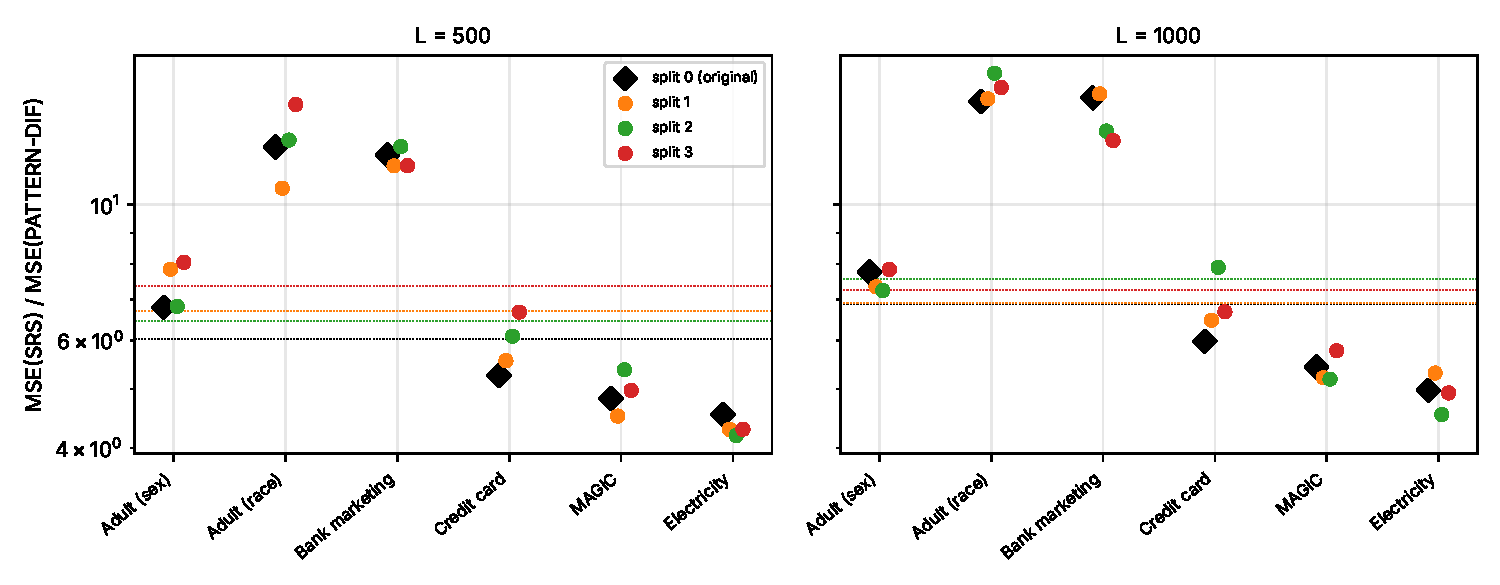
\includegraphics[width=\textwidth]{splits_efficiency}
\caption{Efficiency of PATTERN-DIF against SRS by setting and split. The diamond is the original split. Dotted lines are the medians over the six settings for each split.}\label{fig:split-eff}
\end{figure*}

Table~\ref{tab:split-main} and Figure~\ref{fig:split-eff} show that the efficiency is stable across splits relative to its variation across settings, which ranges from about $4.5$ (Electricity) to about $15$ (Adult with race, Bank) at $L=1000$. The median over settings of the coefficient of variation across the four splits is $0.07$ and the median ratio of the largest to the smallest split value is $1.18$. The largest spreads are Adult (race) at $L=500$ (from $10.6$ to $14.6$) and Credit card at $L=1000$ ($6.0$ to $7.9$). Part of this spread is Monte Carlo error rather than split-to-split variation, because each value rests on $100$ replicates ($200$ for split $0$). Adult (race) and Bank have the highest efficiency and Electricity and MAGIC the lowest in every split and at both budgets. The efficiency of PATTERN-DIF was at least $4.1$ in all $48$ cell-split values.

The median over the six settings is $6.0$, $6.7$, $6.5$ and $7.4$ at $L=500$ for splits $0$ to $3$, and $6.9$, $6.9$, $7.6$ and $7.3$ at $L=1000$. The original split gives the lowest median of the four at both budgets (at $L=1000$ only marginally below split~1), so the headline numbers of the main study are not flattered by the choice of split in these settings; pooling the four splits, the median is $6.7$ at $L=500$ and $7.3$ at $L=1000$ against $6.0$ and $6.9$ for split $0$ alone. This is a difference of at most about $12\%$, small against the factor of 6 to 7 itself. Coverage was unaffected: the mean coverage of the PATTERN-DIF intervals was $0.948$ to $0.951$ on every split ($0.950$ overall), against $0.939$ to $0.941$ for SRS with the plug-in estimator. The worst contrast, in any split, had coverage $0.84$ to $0.88$ for PATTERN-DIF; with $100$ replicates per cell the Monte Carlo standard error of one coverage is $0.02$, so these worst values are partly noise.

These results are limited in three ways. Three new splits and four in total are far fewer than the $20$ that a full study of between-split variation would use, so the spread of Table~\ref{tab:split-main} is a rough indication only. Only the six largest settings were repeated, so the median over all eleven settings of the main study is not recomputed. The nine models share the same families in every split, and the splits do not change the learner seeds or the groups, so variation from other hyperparameters or model families is not addressed.

\section{Comparison with existing labelling designs}\label{sec:baselines}

PATTERN-DIF combines four ingredients that are each known: sampling where models disagree, stratification on a model-based proxy with Neyman-type allocation, design-based ratio estimation and a model-assisted (difference) estimator. This section asks whether a reviewer's natural alternatives, built from one or two of these ingredients, already do as well. This study was run before the final form of the method was fixed: its PATTERN-DIF variant (B5, with $\lambda=1$) is the same estimator as the main method, but the samples differ from those of Section~\ref{sec:empirical} (different random seeds), so medians differ by a few per cent between the two studies. We implemented five families of baselines (B1--B5 below; code in \texttt{tcs/labeling\_baselines.py}, study in \texttt{experiments/label\_baselines.py}) and ran them with SRS and PATTERN on the eleven settings of Section~\ref{sec:empirical}, at $L\in\{250,500,1000,2000\}$ with $L\le N/4$ (35 setting--budget cells) and $R=200$ replications per cell.

\paragraph{Common ground.} To make the comparison about the choice of labels and estimators and nothing else, every method estimates the same vector of totals $T$ (Section~\ref{sec:setting}), plugs it into the same map $\hat\theta=f(\hat T)$ for all $3\binom{M}{2}=108$ comparison estimands $\theta^{\mathrm{TPR}}_{mj},\theta^{\mathrm{FPR}}_{mj},\theta^{\mathrm{ERR}}_{mj}$, and reports 95\% Wald intervals from a linearisation variance. Every method that uses a proxy uses the same $\pi_i=M^{-1}\sum_m\hat p_{mi}$, and every allocation over several estimands uses the same weights $w_k=1/S_k^2$ as \eqref{eq:alloc}. The budget is counted in distinct labelled instances. Pool labels are used only to answer label queries, to compute the truth and, for reporting, to pick the three most accurate models. Estimands whose numerator is identically zero in the pool (the two models never disagree on the relevant instances) are estimated exactly by every design and are left out of all summaries. This removes 51 of the 108 estimands in the law-school setting, including all those among its three most accurate models, and none elsewhere.

\subsection{Baselines}

\paragraph{B1: importance sampling for active comparison.} \citet{sawade2012active} compare the risks of two fixed models by drawing $n$ instances with replacement from an instrumental distribution $q$ and estimating each risk by the self-normalised weighted mean $\sum_k \ell_k/q_k\big/\sum_k 1/q_k$ (with $p(x)=1/N$ on a pool). Their Theorem~1 shows that the asymptotic variance of the estimated risk difference is minimised by $q^*(x)\propto p(x)\{\mathbb E[(\ell_1-\ell_2-\Delta)^2\mid x]\}^{1/2}$. They replace $p(y\mid x)$ by an equal mixture of the models' predictive distributions, and for $k$ models they use the equal mixture of the pairwise-optimal distributions. We keep all of this and change only the quantity being compared. With replacement draws $i_1,\dots,i_n\sim q$, our totals are the Hájek (self-normalised) estimators
\[
\hat T^{\mathrm{IS}}=N\,\frac{\sum_{k=1}^n t_{i_k}(Y_{i_k})/q_{i_k}}{\sum_{k=1}^n 1/q_{i_k}},
\qquad
\hat\theta-\theta\approx\frac1n\sum_{k=1}^n \frac{a_{i_k}}{q_{i_k}},\quad a_i=\nabla f(T)^{\top}\{t_i(Y_i)-T/N\}.
\]
For $\theta^{\mathrm{ERR}}_{mj}$, $a_i=\{|\hat y_{mi}-Y_i|-|\hat y_{ji}-Y_i|-\theta^{\mathrm{ERR}}_{mj}\}/N$, which is exactly Sawade et al.'s centred loss difference. For $\theta^{\mathrm{TPR}}_{mj}$, the self-normalisation is automatic because $f$ is a ratio, and $a_i=\sum_g s_g\,\mathbf 1\{G_i=g\}\,Y_i\{(\hat y_{mi}-\hat y_{ji})-(\mathrm{TPR}_{mg}-\mathrm{TPR}_{jg})\}/P_g$. The asymptotic variance is $n^{-1}\sum_i\mathbb E[a_i^2]/q_i$ \citep{hansen1943}, so the single-estimand optimum is $q_i\propto\{\mathbb E_\pi a_i^2\}^{1/2}$, with the expectation taken under $Y_i\sim\mathrm{Bernoulli}(\pi_i)$ and $a$ evaluated at the proxy totals. This is our adaptation to TPR and FPR gaps. For a pair $(m,j)$ we combine its three estimands as $q^{(mj)}_i\propto\{\sum_{k\in(m,j)}w_k\mathbb E_\pi a_{ik}^2\}^{1/2}$. The design distribution is the equal mixture over the 36 pairs, as in Sawade et al., mixed with the uniform distribution with weight $0.05$ so that every $q_i$ is bounded away from zero. Draws continue until $L$ distinct instances are labelled; repeated draws reuse the label. The median number of draws was $1.12L$ (range $1.02L$--$1.48L$), so B1 effectively gets more than $L$ draws for $L$ labels. The variance is estimated by $n^{-1}$ times the sample variance of $\hat a_{i_k}/q_{i_k}$.

\paragraph{B2: proxy-score stratification.} The classic approach to estimating a classifier's metrics with few labels stratifies on the classifier's score and allocates optimally \citep{bennett2010online,kumar2018classifier}. We form strata as group $\times$ within-group quantile bins of $\pi_i$ (10 bins, Score-10; and 5 bins, Score-5), merge strata smaller than 50 as for PATTERN, and use the same estimator \eqref{eq:HT}, variance \eqref{eq:var} and proxy-Neyman allocation \eqref{eq:alloc}. B2 therefore differs from PATTERN only in the strata. It uses the proxy strongly but ignores which models disagree.

\paragraph{B3: disagreement-focused two-phase design.} Labelling only where models disagree is the ``active $\neq$'' baseline of \citet{sawade2012active} and the discordant-pair approach of \citet{musgrove2023discordant} and of the screening-test literature \citep{pepe2001comparing}. On its own it identifies only ratios, because the denominators $P_g,Q_g$ need labels in the agreement set. Let $D=\{i:0<K_i<M\}$ and $A=U\setminus D$. Phase 1 draws a simple random sample $s_0$ of size $n_0$ from $U$. Phase 2 draws a simple random sample of $L-n_0$ from $D\setminus s_0$. Conditionally on $n_A=|s_0\cap A|$, the labelled units in $A$ are a simple random sample from $A$. Conditionally on $|s_0\cap D|$, the union of $s_0\cap D$ and the phase-2 sample is a simple random sample of size $n_D=|s_0\cap D|+L-n_0$ from $D$. The combined estimator is therefore the two-stratum estimator $\hat T=N_A\bar t_A+N_D\bar t_D$ with variance \eqref{eq:var} at the realised $(n_A,n_D)$, which is conditionally design-unbiased. We take $n_0=L/4$ (Dis-25) and $n_0=L/2$ (Dis-50).

\paragraph{B4: prediction-powered inference.} PPI \citep{angelopoulos2023ppi} corrects the predictions on the whole pool with the labelled residuals. With the prediction of $t_i$ taken as its proxy mean $\tilde t_i=\pi_iu_i+(1-\pi_i)v_i$, the PPI estimator of a total under SRS is the difference estimator
\[
\hat T^{\mathrm{PPI}}_\lambda=\lambda\sum_{i\in U}\tilde t_i+\frac Nn\sum_{i\in s}\{t_i(Y_i)-\lambda\tilde t_i\},
\]
with $\lambda=1$ (PPI). PPI++ \citep{angelopoulos2026ppipp} tunes $\lambda$ for each estimand. In our finite-pool setting the predictions are known for every unit, so the $(1+n/N)$ factor of PPI++ drops out and the variance-minimising value is the regression coefficient of $\nabla f^\top t_i$ on $\nabla f^\top\tilde t_i$ in the sample. We clip it to $[0,1]$. StratPPI \citep{fisch2024stratppi} applies PPI++ within strata with a stratum-specific $\lambda_{hk}$ and allocates the budget by a Neyman rule on the residual standard deviation, estimated from the predictor's own confidence scores. We use the B2 strata (group $\times$ 10 proxy bins), per-stratum and per-estimand $\lambda_{hk}$ clipped to $[0,1]$, and the allocation $n_h\propto N_h\{\sum_k w_k\,\overline{\pi(1-\pi)(A_{k}-B_{k})^2}_h\}^{1/2}$. Here $\pi_i(1-\pi_i)(A_{ik}-B_{ik})^2$ is the proxy variance of the residual $z_{ik}-\mathbb E_\pi z_{ik}$, so this allocation is Fisch et al.'s confidence-based rule for our estimands. In all three versions the variance is the stratified formula \eqref{eq:var} applied to the residuals $z_{ik}-\lambda\,\nabla f^\top\tilde t_i$.

\paragraph{B5: PATTERN with a model-assisted estimator (the proposed method).} The PPI correction is a difference or GREG-type estimator \citep[Chapter~6]{sarndal1992} and can be applied to the PATTERN sample without changing the design. PATTERN-DIF uses the stratified difference estimator with $\lambda=1$. PATTERN-PPI tunes $\lambda_{hk}$ per stratum as in StratPPI. B5 is the proposed method (PATTERN-DIF, $\lambda=1$) and a tuned-weight variant (PATTERN-PPI), and is reported in the last block of the results.

\paragraph{Not run.} Active testing with LURE \citep{kossen2021active}, adaptive variance-minimising selection \citep{hara2024}, and active inference \citep{zrnic2024active,li2025robust} select labels sequentially and target one estimand of one model. Their fixed-budget, one-shot analogue for our vector of estimands is B1, which uses the same proxy-optimal inclusion principle. Model-based estimators that need a fitted joint model of labels and scores (for example SSME) are outside the design-based comparison made here.

\subsection{Results}

\begin{table*}[t]\centering\footnotesize
\caption{Baselines by label budget $L$ (number of settings in brackets). Efficiency: ratio of mean squared errors, median over the non-degenerate comparison estimands within a setting, then median over settings; ``vs SRS'' is MSE(SRS)/MSE(method), ``vs PATTERN'' is MSE(PATTERN)/MSE(method), so values above 1 favour the method. Coverage: nominal 95\% Wald intervals, mean over estimands and settings; ``worst'': lowest single-estimand coverage over all settings and budgets. $R=200$ replications per setting and budget. Source: \texttt{results/label\_baselines.json}.}\label{tab:base-budget}
\setlength{\tabcolsep}{3.5pt}
\resizebox{\textwidth}{!}{\begin{tabular}{lrrrrrrrrrrr}\toprule
 & \multicolumn{2}{c}{$L=250$ (11)} & \multicolumn{2}{c}{$L=500$ (10)} & \multicolumn{2}{c}{$L=1000$ (8)} & \multicolumn{2}{c}{$L=2000$ (6)} & \multicolumn{3}{c}{All $(s,L)$} \\
\cmidrule(lr){2-3} \cmidrule(lr){4-5} \cmidrule(lr){6-7} \cmidrule(lr){8-9} \cmidrule(lr){10-12}
Method & vs SRS & vs PAT. & vs SRS & vs PAT. & vs SRS & vs PAT. & vs SRS & vs PAT. & Cover. & Worst & ms \\ \midrule
SRS & 1 & 0.27 & 1 & 0.25 & 1 & 0.23 & 1 & 0.14 & 0.925 & 0.16 & 8 \\
PATTERN & 3.75 & 1 & 3.95 & 1 & 4.35 & 1 & 7.43 & 1 & 0.947 & 0.52 & 8 \\
IS (B1) & 3.09 & 0.79 & 2.77 & 0.74 & 3.48 & 0.67 & 4.30 & 0.54 & 0.950 & 0.60 & 9 \\
Score-10 (B2) & 1.45 & 0.40 & 2.09 & 0.52 & 2.24 & 0.56 & 4.16 & 0.50 & 0.941 & 0.17 & 8 \\
Score-5 (B2) & 1.97 & 0.54 & 2.24 & 0.57 & 2.15 & 0.52 & 3.18 & 0.43 & 0.943 & 0.37 & 8 \\
Dis-25 (B3) & 2.25 & 0.42 & 2.27 & 0.55 & 2.04 & 0.35 & 2.48 & 0.26 & 0.942 & 0.45 & 9 \\
Dis-50 (B3) & 1.84 & 0.43 & 1.94 & 0.37 & 1.68 & 0.34 & 1.93 & 0.25 & 0.940 & 0.36 & 9 \\
PPI (B4) & 1.82 & 0.49 & 1.82 & 0.47 & 1.86 & 0.44 & 1.81 & 0.27 & 0.940 & 0.27 & 34 \\
PPI++ (B4) & 2.10 & 0.49 & 1.97 & 0.48 & 1.93 & 0.44 & 1.89 & 0.27 & 0.929 & 0.16 & 49 \\
StratPPI (B4) & 3.07 & 1.01 & 4.45 & 1.12 & 4.58 & 1.08 & 8.50 & 0.83 & 0.924 & 0.14 & 44 \\
\midrule \multicolumn{12}{l}{\emph{Extension (B5): PATTERN sample, model-assisted estimator}} \\
PATTERN-DIF (B5) & 6.57 & 1.63 & 6.23 & 1.48 & 6.64 & 1.48 & 15.5 & 1.32 & 0.946 & 0.64 & 35 \\
PATTERN-PPI (B5) & 6.71 & 1.68 & 6.37 & 1.55 & 6.83 & 1.54 & 15.5 & 1.33 & 0.929 & 0.20 & 51 \\
\bottomrule\end{tabular}}\end{table*}


Table~\ref{tab:base-budget} summarises all methods by budget. PATTERN is the most efficient of the designs that use the same plain estimator as SRS (B1 to B3), at every budget: its median efficiency against SRS is 3.75, 3.95, 4.35 and 7.43 at $L=250,500,1000,2000$. It is not the most efficient method overall. StratPPI, which combines proxy strata with a model-assisted estimator, matches or exceeds it in the paired medians at $L=250$, 500 and 1000 (ratios 1.01, 1.12, 1.08) and has the higher median efficiency against SRS at $L=500$, 1000 and 2000 (4.45, 4.58, 8.50), and the extensions B5, which add the same kind of correction to the PATTERN sample, are better than both. Among the competing designs the closest are importance sampling (B1: 3.09, 2.77, 3.48, 4.30 against SRS; 0.54--0.79 of PATTERN) and StratPPI (B4: 3.07, 4.45, 4.58, 8.50; 1.01, 1.12, 1.08, 0.83 of PATTERN). Proxy-score strata alone (B2) reach 1.45--4.16 against SRS, the disagreement-only designs (B3) 1.7--2.5 and PPI/PPI++ with simple random labels 1.8--2.1, all clearly below PATTERN (medians 0.25--0.57 of its efficiency). PPI and PPI++ with SRS labels barely move with $L$ (1.8--2.1): they use the proxy but not the structure that the numerators vanish where models agree. The disagreement-only designs also improve little with the budget (1.7--2.5). A plausible reason is that their agreement-region labels are drawn by SRS at a fixed share of the budget, so the denominators remain noisy, but we did not isolate this effect.

\begin{figure*}[t]\centering
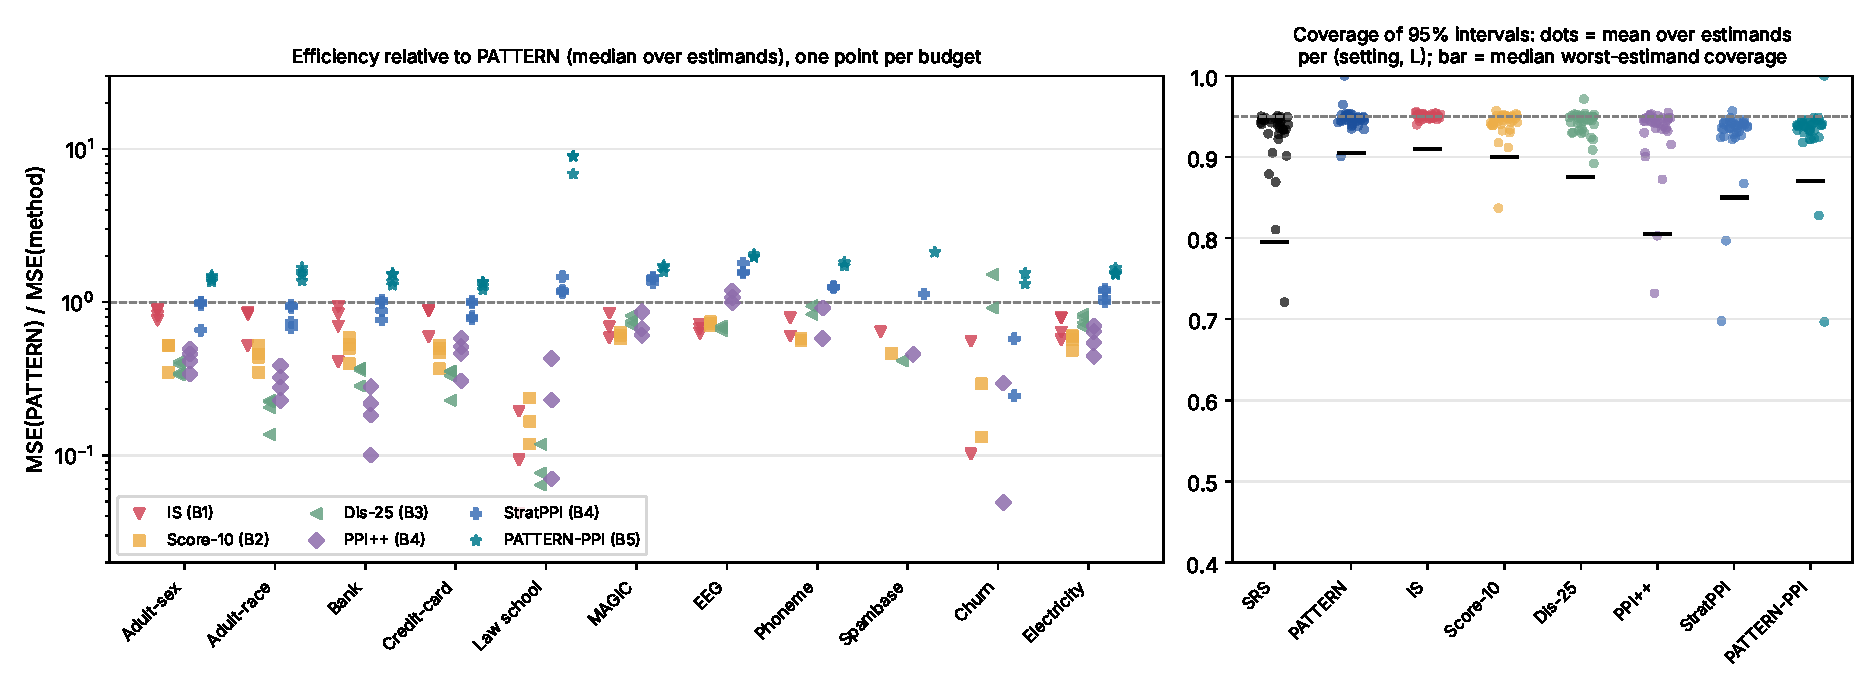
\includegraphics[width=\textwidth]{base_efficiency}
\caption{Left: MSE(PATTERN)/MSE(method) by setting, one point per budget, median over comparison estimands (values above 1 mean that the method beats PATTERN; the axis is clipped to $[0.02,30]$ and law school at $L=2000$ is not shown in range because PATTERN labels the whole disagreement set there). Right: mean coverage of the nominal 95\% interval over estimands for each (setting, $L$), with the median over cells of the worst-estimand coverage as a bar. Source: \texttt{results/label\_baselines.json}.}\label{fig:base-efficiency}
\end{figure*}

\begin{table*}[t]\centering\footnotesize
\caption{Efficiency relative to PATTERN, MSE(PATTERN)/MSE(method), median over estimands, by setting at $L=500$ ($L=250$ for Spambase, whose pool is too small for $L=500$). Values above 1 mean that the method beats PATTERN. Second column: efficiency of PATTERN relative to SRS. Last two columns: mean coverage of the 95\% intervals of StratPPI and of PATTERN-PPI. Source: \texttt{results/label\_baselines.json}.}\label{tab:base-setting}
\setlength{\tabcolsep}{3.5pt}
\resizebox{\textwidth}{!}{\begin{tabular}{l rrrrrrrrrrr}\toprule
 & PAT. & \multicolumn{6}{c}{Baselines (B1--B4) vs PATTERN} & \multicolumn{2}{c}{B5 vs PATTERN} & \multicolumn{2}{c}{Coverage} \\
\cmidrule(lr){3-8}\cmidrule(lr){9-10}\cmidrule(lr){11-12}
Setting & vs SRS & IS & Score-10 & Dis-25 & Dis-50 & PPI++ & StratPPI & PATTERN-DIF & PATTERN-PPI & StratPPI & PAT-PPI \\ \midrule
Adult-sex & 4.19 & 0.89 & 0.52 & 0.39 & 0.37 & 0.46 & 0.97 & 1.45 & 1.49 & 0.935 & 0.939 \\
Adult-race & 7.27 & 0.86 & 0.46 & 0.23 & 0.22 & 0.32 & 0.93 & 1.44 & 1.58 & 0.939 & 0.939 \\
Bank & 8.26 & 0.84 & 0.50 & 0.36 & 0.38 & 0.22 & \textbf{1.03} & 1.47 & 1.52 & 0.941 & 0.933 \\
Credit-card & 3.71 & 0.89 & 0.52 & 0.36 & 0.35 & 0.51 & \textbf{1.01} & 1.28 & 1.35 & 0.937 & 0.933 \\
Law school & 39.0 & 0.09 & 0.24 & 0.08 & 0.08 & 0.23 & \textbf{1.47} & 11.1 & 8.97 & 0.797 & 0.828 \\
MAGIC & 2.93 & 0.69 & 0.63 & 0.75 & 0.63 & 0.67 & \textbf{1.43} & 1.70 & 1.73 & 0.942 & 0.943 \\
EEG & 1.70 & 0.67 & 0.73 & 0.70 & 0.66 & \textbf{1.19} & \textbf{1.57} & 1.98 & 2.05 & 0.926 & 0.939 \\
Phoneme & 3.53 & 0.60 & 0.58 & 0.83 & 0.67 & 0.58 & \textbf{1.26} & 1.71 & 1.72 & 0.946 & 0.941 \\
Spambase$^{\ast}$ & 5.77 & 0.64 & 0.46 & 0.42 & 0.37 & 0.46 & \textbf{1.13} & 2.14 & 2.12 & 0.925 & 0.933 \\
Churn & 34.6 & 0.10 & 0.13 & \textbf{1.52} & 0.28 & 0.05 & 0.24 & 1.28 & 1.32 & 0.930 & 0.932 \\
Electricity & 2.86 & 0.79 & 0.59 & 0.80 & 0.73 & 0.64 & \textbf{1.21} & 1.49 & 1.53 & 0.942 & 0.933 \\
\bottomrule\end{tabular}}\end{table*}


\paragraph{Where a baseline beats PATTERN.} Table~\ref{tab:base-setting} and Figure~\ref{fig:base-efficiency} show where the ranking changes. First, StratPPI beats PATTERN at $L=500$ in seven of the ten settings of the table (ratios 1.01--1.57 in Bank, Credit-card, Law school, MAGIC, EEG, Phoneme and Electricity, and 1.13 in Spambase at $L=250$), and is below it in Adult-sex (0.97), Adult-race (0.93) and Churn (0.24). Over all cells its ratio exceeds 1 in 19 of 35 (median 1.12 at $L=500$). The margin is small in most settings, and it is not a failure of the stratification: StratPPI uses the same sample size but a model-assisted estimator, and B5 shows that the same correction applied to the PATTERN sample improves PATTERN itself by a median factor of 1.3--1.7. Second, Dis-25 beats PATTERN on Churn at $L=500$ (ratio 1.52); there the pool has a 19\% disagreement set, PATTERN strata are mostly small, and Dis-25 labels most of its sample inside the disagreement set. Its intervals are not reliable in that cell: mean coverage 0.93 but worst-estimand coverage 0.66, so the apparent gain should be read with caution. Third, PPI++ beats PATTERN on EEG (ratio 1.19 at $L=500$), the setting with the largest disagreement set (73\%), where agreement cells hold little and the proxy is informative. Importance sampling never beats PATTERN in the all-estimand median (ratio below 1 in all 35 cells), but on the pairs among the three most accurate models it is competitive: its median efficiency against SRS on those pairs is 4.2, 4.1, 4.2 and 6.3 at $L=250,\dots,2000$, against 3.4, 3.6, 4.0 and 6.8 for PATTERN, and it beats PATTERN on those pairs in 10 of 35 cells (Adult-sex: 1.49 at $L=250$ and 1.10 at $L=500$, while its all-estimand ratio there is 0.89). Where the question is only about the best few models, importance sampling is a serious alternative.

\paragraph{Where PATTERN wins clearly.} In the two settings with the lowest disagreement rate, Law school and Churn, PATTERN is 6--84 times more efficient than SRS at $L\le1000$ and PATTERN labels essentially every disagreement instance at $L=2000$ in Law school (all non-degenerate estimands then have error close to zero, ratio above $10^{20}$, so these cells are shown as $>$100 and excluded from the figure range). IS, Dis-50, score strata and PPI++ reach only 0.04--0.7 of PATTERN's efficiency there (Dis-25 on Churn is the exception discussed above), because none of them isolates the agreement region exactly: PATTERN gives it a stratum of its own that can be labelled sparsely, while the other designs either draw it at random or leave the disagreement set under-sampled.

\paragraph{Coverage and failures.} Over all 35 cells the mean 95\% coverage is 0.925 (SRS), 0.947 (PATTERN), 0.950 (IS), 0.941 (Score-10), 0.942 (Dis-25), 0.929 (PPI++), 0.924 (StratPPI), 0.946 (PATTERN-DIF) and 0.929 (PATTERN-PPI). The shortfalls concentrate in the smallest cells. The lowest worst-estimand coverages over all cells are 0.14 for StratPPI (Churn, $L=250$), 0.16 for SRS and for PPI++, 0.17 for Score-10, 0.20 for PATTERN-PPI, 0.45 for Dis-25 and 0.52 for PATTERN (Churn, $L=250$). The tuned estimators (PPI++, StratPPI, PATTERN-PPI) undercover when per-stratum tuning parameters are estimated from a few labels, notably in Law school where PATTERN-PPI covers 0.70 at $L=250$ and StratPPI 0.70--0.87 below $L=2000$. PATTERN-DIF, which fixes $\lambda=1$, keeps the coverage of PATTERN (0.946). Undefined estimates (a group with no sampled positive) occurred in at most 1\% of replications for any method (Dis-25, Adult-race, $L=250$: 1\%; SRS 0.5\%; PATTERN and the others none). Runtimes per replicate (design computation excluded) are 8--11 ms on average for the stratified and importance-sampling designs and 34--51 ms for the PPI-type estimators (Table~\ref{tab:base-budget}, last column), which tune per estimand and stratum. Design computation is at most 0.6 s per cell for every method.

\paragraph{The model-assisted extension.} PATTERN-DIF and PATTERN-PPI (bottom block of Table~\ref{tab:base-budget}) improve on PATTERN in every cell except Law school at $L=2000$, where PATTERN is already exact, by a median factor of 1.3--1.6 (by budget) and up to 11 in Law school at $L\le500$; they are the best methods in this study, with efficiency against SRS of 6.6, 6.2, 6.6 and 15.5 for PATTERN-DIF. The estimated-$\lambda$ version adds little over $\lambda=1$ (PATTERN-PPI is within 3\% of PATTERN-DIF in the median) and costs coverage, so we recommend the fixed-$\lambda$ version if the extension is used. Because the extension changes the estimator rather than the design, its variance expressions are those of the difference estimator under stratified sampling \citep{sarndal1992}; its validity as a design-based method in our setting follows from the known proxy totals, but we did not extend the theory of Section~\ref{sec:theory} to it, and it is reported here as an empirical result.

\paragraph{Limitations.} The comparison is restricted to fixed-budget, one-shot designs on cached pools of nine models with logistic-type probabilities; the proxy is the same for every method, so a better proxy for any of them (for example a calibrated or learned one) could change the ranking, especially for StratPPI and PATTERN-PPI which rely on it directly. The importance-sampling baseline draws with replacement and so spends more than $L$ draws for $L$ labels; counting draws instead of labels would lower its efficiency. $R=200$ replications give Monte Carlo errors of about 10\% on a single mean squared error, so differences between 0.9 and 1.1 in Table~\ref{tab:base-setting} should not be read as ranking. Medians over estimands hide estimand-level differences: on the three types, PATTERN's median efficiency against SRS is 6.2 (TPR), 4.8 (FPR) and 3.8 (ERR), against 3.0, 3.5 and 3.0 for IS and 5.3, 5.2 and 2.3 for StratPPI.

\section{Ablations and robustness}
\label{sec:ablations}

This section varies one ingredient of PATTERN-DIF at a time and asks two questions: does the estimator remain valid, and how much efficiency is gained or lost relative to the default? The default is the method of the main study: strata $(G_i,K_i)$ with strata smaller than 50 merged within group, weighted generalised Neyman allocation \citep{neyman1934} computed with the ensemble-mean proxy $\pi_i$, a floor of 10 labels per stratum, the stratified difference estimator with $\lambda=1$ and the same proxy, and 95\% Wald intervals from the linearisation variance. The estimator that uses the proxy only to allocate labels, the plain (Horvitz--Thompson) estimator, is called HT or $\lambda=0$. Because the proxy now enters the estimator as well as the allocation, the proxy ablations report the two roles separately, and every ablation reports the difference estimator and, where it is informative, HT on the same samples. All results come from \texttt{experiments/label\_ablations\_dif.py} (helpers in \texttt{tcs/labeling\_variants\_dif.py}) and are stored in \texttt{results/label\_ablations\_dif.json}. An earlier version of this study, in which the plain estimator was the default, is not reported; where its conclusions differ they are noted below.

\paragraph{Protocol.} We use the eleven cached pools and budgets $L\in\{250,500,1000\}$ with $L\le N/4$ (29 setting--budget cells) and $R=150$ replications per cell and design. The first seven designs (SRS, GROUP, PATTERN and four alternative stratifiers) draw the same samples as an earlier version of this ablation study that used the plain estimator throughout (\texttt{results/label\_ablations.json} in the repository); we call it the earlier plug-in study and refer to its numbers where they are compared, so that differences between the two studies are due to the estimator alone. There are 108 comparison targets for the 36 pairs of nine models; targets whose numerator vanishes identically in the pool are exact for every design and are excluded (only Law school, where 57 remain). Efficiency is the per-target ratio $\mathrm{MSE}_{\mathrm{SRS}}/\mathrm{MSE}_{\mathrm{design}}$ with SRS and the plain estimator as reference, clipped to $[10^{-4},10^{4}]$, summarised by the median over targets and then over cells. ``Rel.'' is the median over cells of $\mathrm{MSE}_{\mathrm{PATTERN\text{-}DIF}}/\mathrm{MSE}_{\mathrm{variant}}$ (above one favours the variant) and ``Win'' the share of cells with Rel.\ above one. Coverage is the mean over targets and the worst target. With $R=150$ the Monte Carlo standard error of one coverage is about 0.018 and the minimum over 108 targets that all cover exactly 95\% has mean 0.90, so worst-target coverage near 0.90 is consistent with nominal behaviour and values well below 0.88 are not. A design with more strata than the budget can feed at 10 labels each uses the floor $\max(2,\lfloor 0.8L/H\rfloor)$. Undefined estimates occurred in at most 0.7\% of replications.

\subsection{Stratifier (A1)}

Table~\ref{tab:abl-design} varies the stratifier; per-cell values are in Table~\ref{tab:abl-app-eff-design} of the appendix. On the same samples the difference estimator is more efficient than HT in all 29 cells (median ratio 1.67, range 1.36 to 14.5 in Law school), and its efficiency against SRS is 6.3 at every budget, compared with 3.6 to 4.3 for HT. The two gains are not additive: SRS with the difference estimator (SRS-DIF, i.e.\ PPI of \citealt{angelopoulos2023ppi} with the ensemble proxy) gains a factor 1.9, the PATTERN design with HT a factor 4.0 over all budgets, and the product of these medians (7.5) exceeds the combined gain.

The stratifier conclusions of the earlier study carry over. Group $\times$ agree/disagree keeps 74\% of the default's precision (earlier 71\%) and the joint pattern of the three models agreeing most with the ensemble keeps 38\% (earlier 37\%): the count $K_i$ is what matters, and three models cannot isolate the disagreement among 36 pairs. Splitting each $(G,K)$ cell at the median of $\pi_i$ is a tie (Rel.\ 1.01, better in 15 of 29 cells; by budget 0.99, 0.97, 1.04), as are tertile bins (0.99), whose extra strata eat the budget through the floor (3 to 9 labels where it binds). We keep $K_i$. The allocation tailored to the variance of the difference estimator (\texttt{'resid'} in \texttt{tcs.labeling\_dif}) is not better than the plain allocation (Rel.\ 0.96, better in 13 cells). The references that drop an ingredient lose clearly: GROUP-DIF and SRS-DIF keep 28\%, proportional allocation 57\% (earlier 52\%) and the gap-targeted allocation of A5 74\% (earlier 74\%). Coverage hardly depends on the stratifier (mean 0.938 to 0.946).

\begin{table*}[t]
\centering\footnotesize
\caption{Stratifier ablation (A1). Efficiency vs SRS (plain estimator): median over cells of the median over targets of $\mathrm{MSE}_{\mathrm{SRS}}/\mathrm{MSE}$. Rel.: median over the 29 cells of $\mathrm{MSE}_{\mathrm{PATTERN\text{-}DIF}}/\mathrm{MSE}_{\mathrm{variant}}$; Win: share of cells with Rel.\ $>1$. Coverage: mean over cells of the mean over targets (mean) and of the worst target (worst), nominal 0.95. Source: \texttt{results/label\_ablations\_dif.json}.}
\label{tab:abl-design}
\begin{tabular}{lccccccc}
\toprule
 & \multicolumn{3}{c}{Efficiency vs SRS} & & & \multicolumn{2}{c}{Coverage} \\
\cmidrule(lr){2-4}\cmidrule(lr){7-8}
Variant (estimator DIF unless stated) & $L=250$ & 500 & 1000 & Rel. & Win & mean & worst \\
\midrule
PATTERN-DIF (default) & 6.27 & 6.18 & 6.37 & 1.00 & -- & 0.945 & 0.877 \\
\addlinespace
\multicolumn{8}{l}{\emph{A1: stratifier}}\\
Group $\times$ agree/disagree & 4.33 & 4.65 & 4.81 & 0.74 & 0.07 & 0.946 & 0.881 \\
Group $\times$ pattern of 3 models & 2.82 & 2.98 & 3.43 & 0.38 & 0.00 & 0.941 & 0.867 \\
Group $\times K\times$ 2 proxy bins & 6.75 & 6.42 & 7.18 & 1.01 & 0.52 & 0.943 & 0.877 \\
Group $\times K\times$ 3 proxy bins & 6.79 & 5.90 & 6.61 & 0.99 & 0.38 & 0.945 & 0.890 \\
PATTERN, residual allocation & 5.64 & 6.02 & 6.68 & 0.96 & 0.45 & 0.945 & 0.886 \\
\addlinespace
\multicolumn{8}{l}{\emph{References}}\\
GROUP-DIF (strata = group) & 2.10 & 2.04 & 2.07 & 0.28 & 0.00 & 0.941 & 0.850 \\
SRS-DIF (PPI, $\lambda=1$) & 1.83 & 1.91 & 1.92 & 0.28 & 0.00 & 0.938 & 0.844 \\
Proportional allocation (no proxy) & 3.85 & 3.75 & 3.50 & 0.57 & 0.03 & 0.943 & 0.877 \\
Gap-targeted allocation (A5) & 5.36 & 5.26 & 5.22 & 0.74 & 0.00 & 0.941 & 0.866 \\
PATTERN, plug-in (HT) & 3.63 & 3.93 & 4.34 & 0.65 & 0.00 & 0.944 & 0.858 \\
\bottomrule
\end{tabular}

\end{table*}

\subsection{Proxy and the role of $\lambda$ (A2)}

The proxy now has two jobs, and the ablation separates them (Table~\ref{tab:abl-proxy}; Figure~\ref{fig:abl-proxy} in the appendix shows the per-cell spread). The first block uses a proxy $\tilde\pi$ only to allocate labels and analyses the sample with HT. The second uses the same $\tilde\pi$ in the allocation and in the estimator, through the proxy mean $\psi_i=\tilde\pi_iu_i+(1-\tilde\pi_i)v_i$. The third allocates with $\tilde\pi$ but keeps the ensemble proxy in the estimator.

\emph{Allocation only.} As in the earlier study, the allocation is insensitive to the proxy. With HT, every proxy gives a median efficiency of 3.95 to 4.05 against 3.97 for the ensemble mean, including the reversed proxy $1-\pi$, the shuffled proxy and the constant 0.5; allocation by the true labels gives 3.71. With the ensemble proxy kept in the estimator, the alternative allocations keep 99\% to 101\% of the default's precision (Rel.\ in Table~\ref{tab:abl-proxy}, last block), with per-cell ratios between 0.86 and 1.4 except in Churn at $L=500$, where the constant, naive Bayes and shuffled proxies label the small disagreement strata exhaustively and gain factors of 19, 13 and 6 (1.8 for the logistic proxy). The reason is the same as before: the influence values vary within a stratum mainly through the differences $\hat y_{mi}-\hat y_{ji}$, known without labels. What matters in the allocation is that it is Neyman-type rather than proportional (Rel.\ 0.57).

\emph{Proxy in the estimator.} Here the proxy matters. Replacing the ensemble mean by a single model costs 13\% (logistic regression) or 42\% (naive Bayes, whose probabilities are extreme); the constant 0.5 costs 16\%, a shuffled proxy 47\%, a noisy proxy 39\% and the reversed proxy 34\% (Table~\ref{tab:abl-proxy}, middle block). The difference estimator remains unbiased and its coverage is unaffected (mean 0.940 to 0.949), as the theory predicts, so a poor proxy costs efficiency only. A corrupted proxy also removes the gain over HT on the same sample: the median ratio of DIF to HT is 0.96 for the shuffled and noisy proxies and 1.00 for naive Bayes, against 1.67 for the ensemble, and DIF is less efficient than HT in 19, 18 and 15 of 29 cells for these three. The constant keeps most of the gain (ratio 1.40) because $\psi_i$ still carries the known structure of $u_i,v_i$.

\begin{table*}[t]
\centering\footnotesize
\setlength{\tabcolsep}{4pt}
\caption{Proxy ablation (A2). Eff.: median over all 29 cells of the median-over-targets efficiency vs SRS (plain estimator); Rel.: relative to PATTERN-DIF with the ensemble proxy (as in Table~\ref{tab:abl-design}); worst: mean over cells of the worst-target coverage; mean: mean coverage. In the first block the proxy enters only the allocation and the sample is analysed with HT; in the second it enters allocation and estimator; in the third only the allocation, the estimator keeps the ensemble proxy. The true-label proxy is not defined as an estimator proxy (the estimator would be exact).}
\label{tab:abl-proxy}
\resizebox{\textwidth}{!}{\begin{tabular}{lcccccccccc}
\toprule
 & \multicolumn{3}{c}{Proxy in allocation only (HT)} & \multicolumn{4}{c}{Proxy in both (DIF)} & \multicolumn{2}{c}{DIF, ensemble in estimator} \\
\cmidrule(lr){2-4}\cmidrule(lr){5-8}\cmidrule(lr){9-10}
Proxy & Eff. & Rel. & worst & Eff. & Rel. & mean & worst & Eff. & Rel. \\
\midrule
Ensemble mean $\pi$ (default) & 3.97 & 0.65 & 0.858 & 6.27 & 1.00 & 0.945 & 0.877 & 6.27 & 1.00 \\
Single model (logistic) & 3.96 & 0.64 & 0.861 & 5.56 & 0.87 & 0.943 & 0.886 & 6.01 & 0.99 \\
Single model (naive Bayes) & 4.05 & 0.63 & 0.858 & 3.88 & 0.58 & 0.942 & 0.873 & 5.99 & 1.01 \\
Constant 0.5 & 3.97 & 0.62 & 0.850 & 5.71 & 0.84 & 0.940 & 0.858 & 6.01 & 0.99 \\
$\pi$ shuffled within group & 3.95 & 0.62 & 0.854 & 3.70 & 0.53 & 0.949 & 0.889 & 6.12 & 0.99 \\
$\pi$ with logit noise (sd 2) & 4.05 & 0.64 & 0.854 & 3.46 & 0.61 & 0.949 & 0.877 & 5.91 & 0.99 \\
Reversed, $1-\pi$ & 3.99 & 0.63 & 0.859 & 4.38 & 0.66 & 0.941 & 0.872 & 6.23 & 0.99 \\
True labels (allocation only) & 3.71 & 0.64 & 0.865 & -- & -- & -- & -- & 6.01 & 1.00 \\
\addlinespace
Proportional allocation (no proxy in allocation) & 2.05 & 0.38 & 0.819 & 3.75 & 0.57 & 0.943 & 0.877 & -- & -- \\
\bottomrule
\end{tabular}
}
\end{table*}

\emph{The weight $\lambda$.} Table~\ref{tab:abl-lambda} (appendix) compares $\lambda=0$ (HT), $\lambda=1$ (default) and a $\lambda$ tuned per stratum and target on the labelled units and clipped to $[0,1]$ \citep[as in PPI++ and StratPPI;][]{angelopoulos2026ppipp,fisch2024stratppi}. With the ensemble proxy the tuned version is slightly more efficient than $\lambda=1$ (median Rel.\ 1.016, better in 24 of 29 cells; 1.026 at $L=250$) but it undercovers: mean 0.923, worst target 0.799 on average and 0.227 in Law school at $L=250$, against 0.945, 0.877 and 0.633 for $\lambda=1$. The tuned weights are estimated from a few labels per stratum and the variance estimate ignores that. With a degraded proxy the tuned version is the more efficient of the three (shuffled 5.2, noisy 5.1, reversed 5.4, against 3.7, 3.5 and 4.4 at $\lambda=1$ and about 4.0 for HT), because it shrinks the correction, but again at coverage 0.92 to 0.93. Neither alternative is better than $\lambda=1$ with the ensemble proxy in both efficiency and validity, so we keep $\lambda=1$. Tuning is worth considering only when the proxy is known to be poor and some undercoverage is acceptable.

\subsection{Number of compared models (A3)}

For $M\in\{2,3,5\}$ we drew three random subsets of the nine models per size (the subsets of the earlier study), rebuilt strata, proxy and estimands from the subset only, and compared PATTERN-DIF and PATTERN-HT with SRS on the $3\binom{M}{2}$ targets. Subsets in which all models agree on every instance are dropped. Table~\ref{tab:abl-models} and Figure~\ref{fig:abl-models} show, as before, that the gain is governed by the share of the pool on which the compared models disagree rather than by $M$: the Spearman correlation between log efficiency and the disagreement share across the 284 configurations is $-0.72$, $-0.74$ and $-0.76$ at $L=250$, 500 and 1000 (HT: $-0.81$, $-0.78$, $-0.79$), and within settings at $L=250$ it is negative in all eleven (median $-0.43$). At $L=250$ the median efficiency of PATTERN-DIF is 17.2 when the compared models disagree on less than 10\% of the pool, 12.5 for 10 to 20\%, 4.8 for 20 to 40\% and 3.8 above 40\%. What the difference estimator changes is the size of the gain over HT, which grows with $M$ from 1.15 at $M=2$ to 1.67 at $M=9$. The log ratio of DIF to HT is positively correlated with the disagreement share (0.09, 0.19, 0.34 by budget). The correction therefore helps most where the design alone helps least, but it does not remove the dependence on disagreement. Coverage is not affected by $M$ (mean 0.945 to 0.950); the worst-target figures cannot be compared across rows, because the number of targets grows from 3 to 108.

\begin{table*}[t]
\centering\footnotesize
\caption{Number of compared models (A3). Configs: (setting, budget, subset) combinations; Disagr.: median share of the pool on which not all $M$ models agree. Efficiency: median over configurations of the median-over-targets $\mathrm{MSE}_{\mathrm{SRS}}/\mathrm{MSE}$. DIF/HT: median ratio of the two efficiencies on the same sample. Coverage: PATTERN-DIF, Wald.}
\label{tab:abl-models}
\resizebox{\textwidth}{!}{\begin{tabular}{rccccccccc}
\toprule
 & & & \multicolumn{3}{c}{PATTERN-DIF vs SRS} & \multicolumn{1}{c}{PATTERN-HT vs SRS} & & \multicolumn{2}{c}{Coverage (DIF)} \\
\cmidrule(lr){4-6}\cmidrule(lr){9-10}
$M$ & Configs & Disagr. & $L=250$ & 500 & 1000 & all $L$ & DIF/HT & mean & worst \\
\midrule
2 & 87 & 0.133 & 9.48 & 12.58 & 9.28 & 8.37 & 1.15 & 0.950 & 0.933 \\
3 & 84 & 0.193 & 8.29 & 10.70 & 8.57 & 6.44 & 1.27 & 0.949 & 0.919 \\
5 & 84 & 0.294 & 7.62 & 6.64 & 7.08 & 4.78 & 1.52 & 0.946 & 0.904 \\
9 & 29 & 0.396 & 6.27 & 6.18 & 6.37 & 3.97 & 1.67 & 0.945 & 0.877 \\
\bottomrule
\end{tabular}
}
\end{table*}

\begin{figure*}[t]
\centering
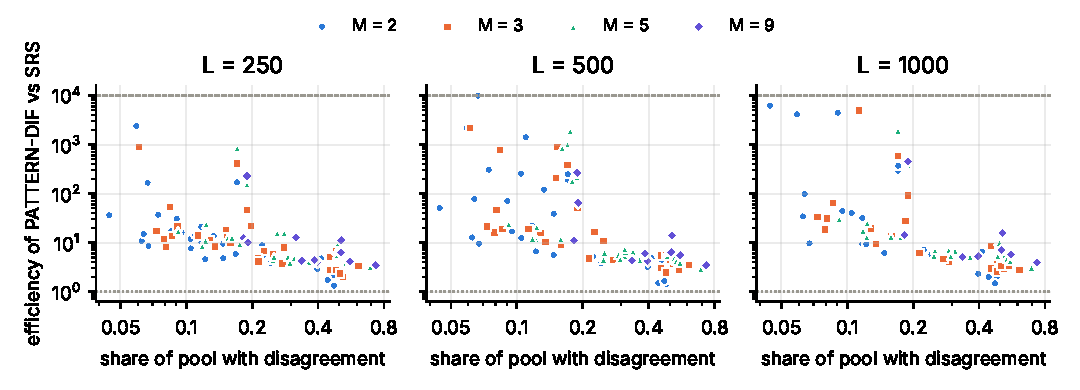
\includegraphics[width=\textwidth]{abl_dif_models_disagreement}
\caption{Efficiency of PATTERN-DIF relative to SRS (median over targets) against the share of the pool on which the compared models do not all agree, for random subsets of $M$ models in every setting (A3). Both axes are logarithmic; the dotted line marks parity and the dashed line the clipping value $10^4$.}
\label{fig:abl-models}
\end{figure*}

\subsection{Small-sample inference (A4)}

With the plain estimator the main study found worst-target coverage near 0.5 at $L=250$ in Churn and Law school, traced to strata whose sampled units show no variation in the influence values. The difference estimator removes most of this: the residual $\xi_i=t_i-\psi_i=(Y_i-\pi_i)(u_i-v_i)$ varies even when no positive is sampled, no (replication, target) pair had a standard error of exactly zero (plain estimator: up to 1.0\% in Law school), and the worst-target Wald coverage in Churn at $L=250$ rises from 0.47 to 0.91 (Table~\ref{tab:abl-inference}, Figure~\ref{fig:abl-coverage}). The shortfalls that remain are of a different kind. Over the 29 cells the worst-target Wald coverage is below 0.85 in five cells (Law school 0.63, MAGIC 0.78 and Adult-sex 0.82 at $L=250$, Bank 0.83 and Phoneme 0.83 at $L=500$), against five cells for HT and six for SRS-DIF. The worst target is a TPR contrast in 17 of 29 cells (FPR in 4, error difference in 8). On average over cells its mean standard error is 0.90 of the Monte Carlo standard deviation (0.99 for the median target) and its bias is below 0.16 standard deviations, so the intervals are too short rather than off-centre, which is consistent with a linearisation error in a ratio with few sampled positives in the smaller group (we did not test this further).

None of the standard corrections closes this gap. A $t$ quantile with \citet{satterthwaite1946} degrees of freedom adds 1\% to the width and moves the mean worst target at $L=250$ from 0.852 to 0.865. The stratified bootstrap percentile interval \citep{efron1979}, which resamples labelled residuals within strata ($B=999$, no finite-population correction; \citealt{raowu1988} discuss a rescaled version), is 11\% wider and a little conservative (mean coverage 0.961 over all cells), with worst target 0.878 and minimum 0.767. The proxy variance floor of \texttt{tcs.labeling\_dif} replaces the sample variance of a stratum by its proxy residual variance when the former is exactly zero ('zero') or by the larger of the two in every stratum ('max'). The 'zero' floor leaves the width unchanged (1.002) and lifts the minimum over cells from 0.633 to 0.780, entirely through Law school (0.90 at $L=250$); combined with the $t$ quantile the mean worst target is 0.885 and four cells stay below 0.85. Only the 'max' floor reaches 0.92 in every cell (mean worst target 0.948), and it is conservative: mean coverage 0.985 at $L=250$, width 1.67 times Wald on average, 1.25 in the median and 4.9 in Law school. For SRS-DIF Wald coverage is poor (minimum 0.27) and the bootstrap worse (0.10); 'max' repairs it (minimum 0.88) at 23\% extra width. The floors were designed after seeing the failure of the plain estimator on these pools, so the 'zero' result for Law school is in-sample (the residual floor is discussed further in Section~\ref{sec:simulation}).

\begin{table*}[t]
\centering\footnotesize
\setlength{\tabcolsep}{4pt}
\caption{Small-sample inference for PATTERN-DIF (A4). Mean: mean over cells and targets; worst: mean over cells of the worst-target coverage; min: minimum over cells of the worst-target coverage. Small pools: Churn, Spambase, Phoneme, Law school. Width: average interval width relative to Wald over all 29 cells. Floors: 'zero' replaces a zero stratum variance by the proxy residual variance, 'max' uses the larger of the two in every stratum.}
\label{tab:abl-inference}
\begin{tabular}{lcccccccc}
\toprule
 & \multicolumn{3}{c}{$L=250$, all} & \multicolumn{2}{c}{$L=250$, small} & \multicolumn{2}{c}{$L\ge 500$} & \\
\cmidrule(lr){2-4}\cmidrule(lr){5-6}\cmidrule(lr){7-8}
Method & mean & worst & min & worst & min & worst & min & Width \\
\midrule
Wald (default) & 0.941 & 0.852 & 0.633 & 0.827 & 0.633 & 0.892 & 0.833 & 1.00 \\
Wald + floor 'zero' & 0.947 & 0.876 & 0.780 & 0.893 & 0.873 & 0.893 & 0.833 & 1.00 \\
Wald + floor 'max' & 0.985 & 0.948 & 0.920 & 0.953 & 0.933 & 0.939 & 0.920 & 1.67 \\
$t$, Satterthwaite df & 0.945 & 0.865 & 0.700 & 0.850 & 0.700 & 0.893 & 0.833 & 1.01 \\
$t$ + floor 'zero' & 0.950 & 0.885 & 0.787 & 0.905 & 0.887 & 0.894 & 0.833 & 1.01 \\
Stratified bootstrap & 0.950 & 0.878 & 0.767 & 0.893 & 0.767 & 0.918 & 0.860 & 1.11 \\
\addlinespace
\multicolumn{9}{l}{\emph{References}} \\
SRS-DIF (PPI), Wald & 0.934 & 0.818 & 0.267 & 0.725 & 0.267 & 0.860 & 0.400 & 1.00 \\
SRS-DIF, Wald + floor 'max' & 0.976 & 0.929 & 0.900 & 0.942 & 0.900 & 0.929 & 0.880 & 1.23 \\
SRS-DIF, bootstrap & 0.924 & 0.741 & 0.100 & 0.678 & 0.100 & 0.818 & 0.153 & 1.12 \\
PATTERN plug-in (HT), Wald & 0.940 & 0.807 & 0.473 & 0.728 & 0.473 & 0.890 & 0.800 & -- \\
\bottomrule
\end{tabular}

\end{table*}

\begin{figure*}[t]
\centering
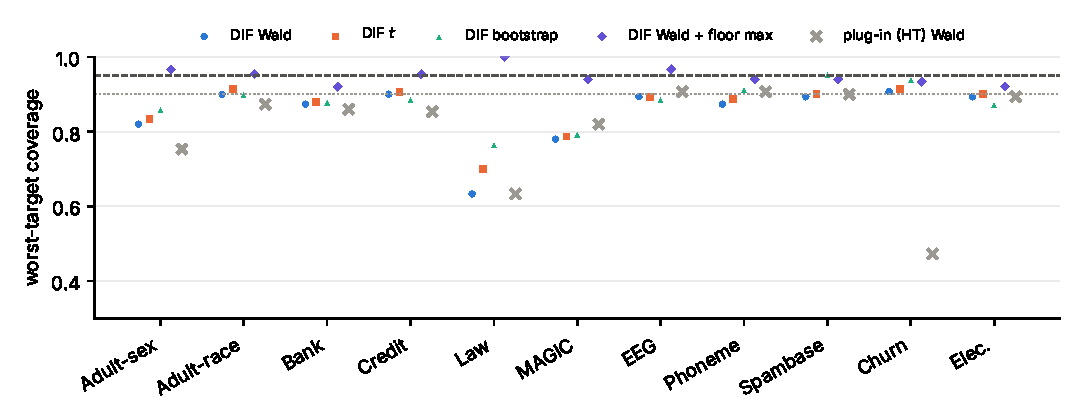
\includegraphics[width=\textwidth]{abl_dif_coverage_L250}
\caption{Worst-target coverage at $L=250$ in each setting for PATTERN-DIF under four interval methods and for the plain estimator (A4). Dashed line: nominal 0.95; dotted line: expected minimum over 108 targets of 150-replicate coverage if every target covered exactly 95\% (0.90; Law school has 57 targets).}
\label{fig:abl-coverage}
\end{figure*}

\subsection{Ranking models by the equalised-odds gap (A5)}

Practitioners also look at each model's equalised-odds gap $EO_m=\max(|\Delta^{TPR}_m|,|\Delta^{FPR}_m|)$ \citep{hardt2016} and rank models by it. We computed the plug-in $\widehat{EO}_m=f_{EO}(\hat T)$ from the totals of the same samples, with the difference estimator (DIF totals) and the plain estimator, and recorded the RMSE, the probability $P$ that the model with the smallest estimated gap has the smallest true gap, Kendall's $\tau$ \citep{kendall1938} between estimated and true gaps, and the bias. We also include a variant of PATTERN whose allocation targets the $2M$ per-model gaps instead of the comparison contrasts (gap-targeted). Table~\ref{tab:abl-eo} summarises the results; per-cell values are in Table~\ref{tab:abl-app-eo}.

The plug-in $\widehat{EO}_m$ is biased upwards, as a maximum of absolute values must be (mean bias 0.042 for SRS, 0.026 for PATTERN with HT, 0.024 for PATTERN-DIF, 0.019 for the gap-targeted variant with DIF). PATTERN-DIF is more accurate than SRS in the median (efficiency 1.94 to 2.21) and identifies the best model more often (mean $P$ 0.50 against 0.35 at $L=250$; 0.46 against 0.21 without Law school, where six models tie, and EEG, where the best model leads by 0.039). PATTERN with HT reaches efficiency 1.80 to 1.94 and $P$ 0.46 to 0.62, so the difference estimator adds little for this purpose. The gain is not uniform: PATTERN-DIF is less accurate than SRS in all Electricity cells (0.57 to 0.73) and in MAGIC at $L=1000$, because the allocation spends labels on disagreement whereas the gap of one model depends on all of its positive predictions. SRS-DIF has about the same RMSE efficiency (2.08 to 2.28) but a lower $P$ (0.42 at $L=250$) and $\tau$ (0.41). The gap-targeted allocation with the difference estimator is the best design here (efficiency 2.30 to 2.61, $P=0.49$, 0.56, 0.65 and $\tau=0.48$, 0.54, 0.64 by budget; never worse than SRS except in Law school) but it keeps only 74\% of the precision for the comparison contrasts (Table~\ref{tab:abl-design}). In Law school the models are near-perfect and six have $EO_m=0$ exactly; the plain estimator then returns exactly zero for them and wins every tie, whereas the difference estimator does not (MSE ratio clipped at $10^{-4}$). When the true margin to the next model is 0.002 or less (Adult-sex, Bank, Credit card default, Churn) identification is hard for every design: $P$ for PATTERN-DIF is at most 0.55 at the largest budget and 0.11 in Credit card default (margin 0.0003).

\begin{table*}[t]
\centering\footnotesize
\setlength{\tabcolsep}{4pt}
\caption{Equalised-odds gap (A5). Eff.: median over cells of the median over models of $\mathrm{MSE}_{\mathrm{SRS}}/\mathrm{MSE}$ for $\widehat{EO}_m$ (cells in which both are exactly zero are skipped); $P$: mean probability that the estimated smallest-gap model has the smallest true gap; $\tau$: mean Kendall $\tau$ between estimated and true $EO_m$. DIF: totals from the difference estimator; plug-in: plain estimator.}
\label{tab:abl-eo}
\begin{tabular}{lccccccccc}
\toprule
 & \multicolumn{3}{c}{$L=250$} & \multicolumn{3}{c}{$L=500$} & \multicolumn{3}{c}{$L=1000$} \\
\cmidrule(lr){2-4}\cmidrule(lr){5-7}\cmidrule(lr){8-10}
Design & Eff. & $P$ & $\tau$ & Eff. & $P$ & $\tau$ & Eff. & $P$ & $\tau$ \\
\midrule
SRS (plug-in) & 1.00 & 0.35 & 0.32 & 1.00 & 0.42 & 0.39 & 1.00 & 0.49 & 0.48 \\
SRS-DIF (PPI) & 2.08 & 0.42 & 0.41 & 2.22 & 0.47 & 0.45 & 2.28 & 0.53 & 0.55 \\
GROUP, plug-in & 1.07 & 0.37 & 0.34 & 1.10 & 0.43 & 0.42 & 1.63 & 0.51 & 0.52 \\
PATTERN, plug-in (HT) & 1.83 & 0.46 & 0.45 & 1.80 & 0.51 & 0.49 & 1.94 & 0.62 & 0.62 \\
PATTERN-DIF (default) & 1.94 & 0.50 & 0.48 & 1.94 & 0.53 & 0.51 & 2.21 & 0.61 & 0.62 \\
Gap-targeted, plug-in & 2.03 & 0.44 & 0.43 & 2.29 & 0.52 & 0.51 & 2.54 & 0.59 & 0.61 \\
Gap-targeted, DIF & 2.30 & 0.49 & 0.48 & 2.61 & 0.56 & 0.54 & 2.51 & 0.65 & 0.64 \\
ORACLE-ALLOC, DIF & 2.02 & 0.50 & 0.47 & 1.77 & 0.54 & 0.52 & 1.93 & 0.57 & 0.60 \\
\bottomrule
\end{tabular}

\end{table*}

\paragraph{Summary.} With the difference estimator the ablation conclusions about the design are those of the earlier plug-in study: the count $K_i$ is the stratifier worth having, Neyman rather than proportional allocation matters, the allocation is insensitive to the proxy, and the gain depends on how often the compared models disagree. Three things differ. First, the proxy now matters in the estimator, where a poor proxy costs up to half of the efficiency and removes the advantage over HT, although coverage is unaffected; the ensemble mean was never beaten there. Second, the difference estimator removes the zero-variance failure of the plain estimator, so the proxy variance floor has become a cheap safeguard ('zero', no loss of width) rather than a 19\% widening, and the remaining undercoverage of rate contrasts at $L=250$ is not fixed by $t$ quantiles, the bootstrap or the floor; only the conservative 'max' floor reaches nominal worst-target coverage. Third, for ranking models by $EO_m$ itself the gap-targeted allocation with the difference estimator is better than the default. Neither tuned $\lambda$ nor proxy-bin strata beat the default consistently, and we keep it; we recommend reporting the Wald interval with the 'zero' floor, which costs nothing in width.

\subsection{Target of inference: the pool or the population}\label{sec:population}

The intervals of Section~\ref{sec:design} cover the contrast computed on the pool, $\theta_U=f(T_U)$. If the pool is itself a sample of $N$ units from a deployment population, the quantity of interest is the population contrast $\theta_{\rm pop}=\tilde f(\tau)$, $\tau=\mathrm E\,t_i(Y_i)$, and the pool-conditional interval ignores the sampling error of the pool. Write $\hat\theta=f(T_{\rm dif})$ for the unchanged estimator. Then
\[
\hat\theta-\theta_{\rm pop}=\underbrace{f(T_{\rm dif})-f(T_U)}_{\text{design error}}+\underbrace{f(T_U)-f(N\tau)}_{\text{pool error}} .
\]
Given the pool, the first term has mean zero to first order and variance $V_{\rm design}=\sum_h N_h^2(1-n_h/N_h)S_h^2(e)/n_h$, the quantity estimated in Section~\ref{sec:design}. The second term is, to first order, a sum of $N$ independent influence values, so the two terms are uncorrelated and
\begin{equation}\label{eq:pop-variance}
V_{\rm total}=\mathrm E\,V_{\rm design}+V_{\rm pool},\qquad V_{\rm pool}=N\,\mathrm{Var}(z_i),\quad z_i=G^{\top}\bigl(t_i(Y_i)-\tau\bigr),
\end{equation}
with $G=\nabla f(N\tau)$ the gradient on the scale of totals. This is the two-phase decomposition of \citet{sarndal1987}. The influence value $z_i$ is that of the full-label plug-in contrast, not the residual $e_i$ of the difference estimator: the proxy removes variance from the labelled part of the error but cannot remove the variation of $Y$ across units of the population, so $V_{\rm pool}$ is the same for every labelling design and every proxy, to first order.

Since the labelled sample is a stratified sample of the pool, $V_{\rm pool}$ is estimated with the weights $w_i=N_h/n_h$:
\[
\hat V_{\rm pool}=\sum_{i\in s}w_i\,(\hat z_i-\bar z)^2,\qquad \bar z=\frac1N\sum_{i\in s}w_i\hat z_i,\qquad \hat z_i=\hat G^{\top}t_i(Y_i),
\]
with $\hat G=\nabla f(T_{\rm dif})$, and the two-phase interval is $\hat\theta\pm1.96\sqrt{\hat V_{\rm design}+\hat V_{\rm pool}}$. The derivation is in \texttt{docs/two\_phase\_note.md} and the code in \texttt{tcs/labeling\_two\_phase.py}. Let $\rho=V_{\rm pool}/V_{\rm design}$. It is of the order of $L\,\mathrm{Eff}/N$, where $\mathrm{Eff}$ is the efficiency of the design against SRS, so it grows with the budget and with the efficiency of the design, and shrinks with the pool size. With correct $V_{\rm design}$ and normal errors the pool-conditional interval has coverage about $2\Phi(1.96/\sqrt{1+\rho})-1$ of the population contrast, which is $0.93$ at $\rho=0.2$, $0.83$ at $\rho=1$ and $0.67$ at $\rho=3$. Efficiency claims change in the same way: the pool term is shared by SRS and PATTERN-DIF, so against the population contrast the MSE ratio is $(\mathrm{Eff}+\rho)/(1+\rho)$, with $\rho$ evaluated for PATTERN-DIF, rather than $\mathrm{Eff}$. For $\mathrm{Eff}=6$ and $\rho=1.5$ this is $3$. This is an arithmetic consequence of \eqref{eq:pop-variance}, not an estimate from the experiments of the earlier sections.

\subsubsection*{Experiment}
We checked the two intervals against population values. The population is the generative model of the non-smooth simulation (five Gaussian covariates, a group with prevalence $0.3$, a logistic label model) with nine fixed scoring rules, so there are $36$ pairs and $108$ contrasts, $\theta^{TPR}$, $\theta^{FPR}$ and $\theta^{ERR}$. Population values were computed on $6\times10^{6}$ draws. For every replicate a new pool of $N\in\{2000,8000,20000\}$ units is drawn and then a PATTERN sample of $L\in\{250,500,1000,2000\}$ labels ($L\le N/4$; ten cells), with the plain allocation and the mean-probability proxy; $R=300$ replicates per cell. Table~\ref{tab:pop-check} and Figure~\ref{fig:pop-check} give the coverage, averaged over the $108$ contrasts and for the worst contrast, together with the median over contrasts of $\hat V_{\rm pool}/\hat V_{\rm design}$ (source: \texttt{results/two\_phase\_check.json}).

\begin{table*}[t]
\centering\footnotesize
\caption{Coverage of the population contrast (nominal $0.95$) over $108$ contrasts, $R=300$ pools per row. $V_{\rm pool}/V_{\rm des}$ is the median over contrasts of the estimated ratio. The last column is the coverage of the pool value by the pool-conditional interval. Source: \texttt{results/two\_phase\_check.json}.}\label{tab:pop-check}
\begin{tabular}{rr r rr rr r}\toprule
 & & & \multicolumn{2}{c}{Pool-conditional} & \multicolumn{2}{c}{Two-phase} & Pool value \\
$N$ & $L$ & $V_{\mathrm{pool}}/V_{\mathrm{des}}$ & mean & worst & mean & worst & (pool-cond.) mean \\\midrule
2{,}000 & 250 & 0.50 & 0.899 & 0.86 & 0.949 & 0.92 & 0.949 \\
 & 500 & 1.51 & 0.809 & 0.72 & 0.952 & 0.92 & 0.948 \\
\addlinespace
8{,}000 & 250 & 0.11 & 0.940 & 0.91 & 0.951 & 0.92 & 0.952 \\
 & 500 & 0.25 & 0.921 & 0.87 & 0.947 & 0.90 & 0.948 \\
 & 1000 & 0.58 & 0.889 & 0.83 & 0.950 & 0.92 & 0.945 \\
 & 2000 & 1.57 & 0.792 & 0.64 & 0.949 & 0.92 & 0.953 \\
\addlinespace
20{,}000 & 250 & 0.04 & 0.940 & 0.90 & 0.945 & 0.91 & 0.945 \\
 & 500 & 0.09 & 0.942 & 0.90 & 0.952 & 0.91 & 0.953 \\
 & 1000 & 0.20 & 0.928 & 0.89 & 0.947 & 0.92 & 0.949 \\
 & 2000 & 0.44 & 0.903 & 0.83 & 0.949 & 0.91 & 0.949 \\
\bottomrule\end{tabular}

\end{table*}

\begin{figure*}[t]
\centering
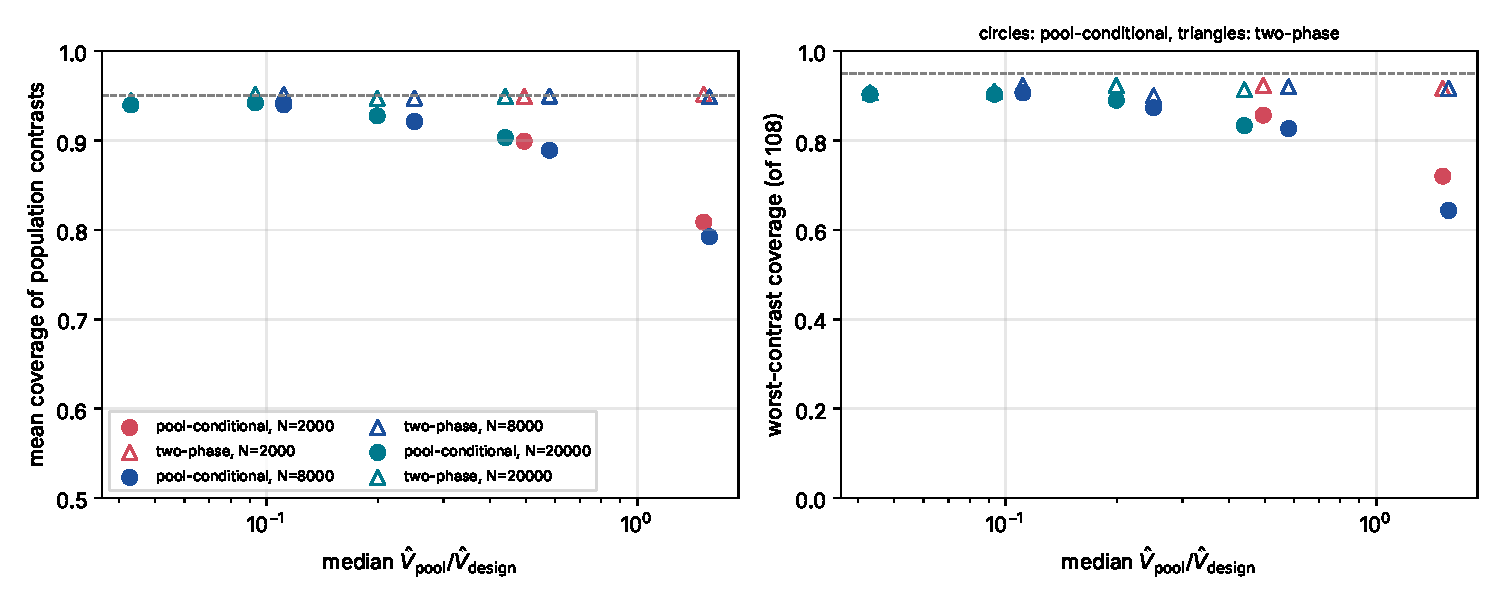
\includegraphics[width=\textwidth]{two_phase_check}
\caption{Coverage of the population contrasts against the median ratio $\hat V_{\rm pool}/\hat V_{\rm design}$, one point per $(N,L)$ cell. Left: mean over the $108$ contrasts. Right: worst contrast. Circles: pool-conditional intervals, triangles: two-phase intervals; colours give $N$.}\label{fig:pop-check}
\end{figure*}

The pool-conditional interval keeps its coverage of the pool value (mean $0.945$ to $0.953$ in all ten cells), so the earlier results are not affected. Against the population contrast its mean coverage falls with $\rho$: $0.94$ when $\rho\le0.11$, $0.90$ to $0.93$ for $\rho$ between $0.2$ and $0.5$, $0.89$ at $\rho=0.58$ and $0.79$ to $0.81$ at $\rho\approx1.5$ (the cells $N=2000,L=500$ and $N=8000,L=2000$), where the worst contrast is covered in $0.72$ and $0.64$ of the replicates. This is close to the value predicted by the formula above. The two-phase interval has mean coverage $0.945$ to $0.952$ in every cell and worst-contrast coverage $0.90$ to $0.92$. The worst of $108$ contrasts with $300$ replicates has a Monte Carlo standard error of $0.013$, so the worst value is expected to lie near $0.92$ even for exact intervals; we do not read the remaining gap as a failure, but the experiment cannot exclude a small one. The price is width: the two-phase interval is $2\%$ to $10\%$ wider when $\rho\le0.2$, $12\%$ wider at $\rho=0.25$ and $21\%$ to $71\%$ wider when $\rho\ge0.44$ (median width over contrasts).

\subsubsection*{When the pool term matters}
It does not matter when $N$ is large against the budget: at $N=20000$ and $L\le500$, $\rho\le0.09$ and the two intervals are nearly the same. It matters when the labelled fraction is not small, which is the regime of the small pools of the empirical study (pools of about $2000$ to $20000$ instances with budgets up to $2000$). The empirical MSE of $\hat\theta$ around the population contrast was $1.04$ to $2.6$ times its MSE around the pool contrast in these cells. Three limits apply. The simulation is stylised, the pool is exactly an independent sample of the population, and the models are fixed and independent of the pool; with real data the deployment population is unknown, the pool may be a convenience sample, and the two-phase interval is then only as good as the assumption that the pool is representative. If the pool is the whole deployment set, the pool-conditional interval is the right one and the two-phase interval is conservative. The gain of PATTERN-DIF over SRS also shrinks for the population target, as shown above, although the ranking of designs does not change. We did not run the full pipeline (training, pooling, labelling) against full-data references on the OpenML data; the check above separates the pool-sampling term from other sources of error by using a known population.

\section{Practical guidance}\label{sec:guidance}

This section turns the results into a procedure that an analyst can follow when comparing a small set of candidate classifiers on fairness and accuracy with a limited labelling budget.

\paragraph{Step 1: describe the agreement structure before labelling.} Compute $K_i$ and the stratum sizes $N_h$ on the unlabeled pool, and the pairwise disagreement rates of the models to be compared. These numbers are free and predict the benefit of the design: in our data, disagreement rates below 5\% went with efficiencies of 5.4 to 15.0 at $L=1000$ (law school excluded), while rates of 8.6\% went with efficiencies of 3.8 to 5.0. If the candidate models disagree on a large share of the pool, the design still helps, but the gain is modest.

\paragraph{Step 2: check that the minority cells are not empty.} Every group-wise rate needs positive and negative instances in each group. The proxy probabilities give an expected count of positives per group and stratum before any label is collected; if the expected number of minority positives in the pool is very small, no design can estimate the corresponding rates, and the estimand should be reconsidered (for example by merging groups).

\paragraph{Step 3: choose the estimands and allocate.} Use the signed contrasts \eqref{eq:theta} for the pairs of interest. If only a few pairs matter, restricting the estimand set to them concentrates labels further. Compute the allocation \eqref{eq:alloc} with the average predicted probability as proxy, at least ten labels per stratum, draw the instances in each stratum without replacement and label them.

\paragraph{Step 4: estimate and report uncertainty.} Estimate the totals with the difference estimator \eqref{eq:DIF}, which corrects the pool-wide proxy total by the labelled residuals and needs no tuning, and report the contrasts with standard errors and intervals. If the statement is about the deployment population rather than about the pool itself, add the pool-sampling variance (Section~\ref{sec:population}): the pool-conditional intervals undercover once the labelling budget is a sizeable fraction of the pool, with coverage of the population contrast down to 0.79 when the variance ratio exceeds one, while the two-phase intervals kept it near 0.95. For budgets below about 500 labels or pools below a few thousand instances, use the more conservative interval options of Section~\ref{sec:ablations} and report the stratum sample sizes, so that readers can judge how many minority positives informed each rate.

\paragraph{Step 5: decide.} A contrast whose interval excludes zero supports a statement that one model has a smaller gap than the other on the stated metric. When no interval excludes zero, the honest conclusion is that the budget did not resolve the comparison; the stratum-level variances computed in Step 3 indicate how many additional labels would be needed, since the variance of every contrast decreases in proportion to the budget for a fixed allocation.

\paragraph{When not to use the design.} The design compares fixed models; it does not help to estimate a single model's fairness more precisely than a group-stratified design does, because a single model's group-wise rates do not depend on disagreements with other models. It also assumes that the group attribute is observed for the whole pool. When the attribute is missing for some instances, it can be added as a third stratum level, but the fairness estimands then refer only to instances with a recorded group.

\section{Discussion}\label{sec:discussion}

\paragraph{Summary.} Comparing classifiers on group-fairness criteria is expensive in labels because the relevant information sits in small cells: positives and negatives of the minority group, and instances on which the models disagree. PATTERN-DIF stratifies the pool by group and by the number of models predicting the positive class, allocates labels with a proxy-based generalised Neyman rule, and estimates the contrasts with a difference estimator that corrects the pool-wide proxy total by the labelled residuals. Across eleven data settings with nine models it reduced the labels needed for a given accuracy by a median factor of 5.8 at 250 labels, 6.3 at 500, 6.9 at 1,000 and 15.5 at 2,000 (5.5, 5.8, 6.0 and 9.4 without the degenerate law-school setting). The stratification contributes more than the estimator (a factor of 3.3 to 8.6 against 1.3 to 1.65), and the two are complementary. Stratifying by group alone gave no gain with the plain estimator. The design needs no label to set up, keeps the design-based guarantees of stratified sampling, and its benefit can be forecast from the disagreement rate of the candidate models before any label is collected.

\paragraph{What the results do and do not show.} The efficiency figures are ratios of mean squared errors against simple random sampling on pools with known labels, so they say how many fewer labels the design needs to reach the same accuracy on the same pool. They do not say that eleven data sets are representative of all comparisons an analyst will face. The gain depends on the disagreement of the compared models: it was between 3.7 and 5.8 at 500 labels for the settings with the highest disagreement (8.6\% to 9.5\%), and larger where the models are nearly identical. The estimator helps because the average predicted probability of nine models is informative in these data (area under the ROC curve 0.76 to 1.00) and, outside EEG, reasonably calibrated (10-bin calibration error 0.02 to 0.07); an uninformative or inverted proxy removes the advantage of the difference estimator over the plain one (Section~\ref{sec:ablations}), and the theory shows that it loses whenever the within-stratum regression slope of the true influence on its proxy falls below one half (Section~\ref{sec:theory}). The allocation, in contrast, is insensitive to the proxy.

\paragraph{Relation to earlier work.} Sampling where models disagree is not new. It is the central idea of active comparison of prediction models \citep{sawade2012active}, and verification designs that oversample discordant results have been used to compare diagnostic tests in medicine for decades. Model-assisted estimation with predictions, including stratified versions, is the subject of prediction-powered inference \citep{angelopoulos2023ppi,fisch2024stratppi}. A stratified prediction-powered estimator, which stratifies by the proxy score, did not beat PATTERN-DIF in the paired median ratio of mean squared errors in any of the 35 cells of the main study (0.5 to 0.6 by budget, Section~\ref{sec:empirical}); its median efficiency against SRS exceeds that of PATTERN-DIF in one cell, Bank at 2,000 labels. What is specific to the present setting is that the estimands are ratios whose numerators depend on disagreements and whose denominators depend on group prevalence everywhere, that many contrasts across several models must be estimated from one sample, and that the group is known before labelling. The stratification by the count of positive predictions, the allocation rule and the difference estimator together handle all three at once.

\paragraph{Limitations.} Several limitations qualify the results. First, the experiments use one split, one set of nine models and pools of 1,841 to 19,537 instances per setting; larger and more diverse collections of models would change the disagreement structure and with it the gain. Second, in six of the eleven settings the group is arbitrary, so these settings test the statistics of the design rather than any fairness question. Third, the intervals are asymptotic. Mean coverage was 0.94 to 0.95, but at 250 labels the worst-covered contrast, in the law-school setting, had coverage 0.59; a variance floor for strata whose sampled labels are all equal raised it to 0.82, and only a conservative version reached the nominal level, at a cost of intervals that are 25\% wider in the median and 67\% wider on average (Section~\ref{sec:ablations}). The floor was designed after seeing these failures, so its benefit is in-sample. Fourth, the primary estimands are signed gaps; the equalised-odds gap is a non-smooth function of them, and the design is a compromise for ranking models by it (Section~\ref{sec:ablations}). Fifth, inference is about the fixed models on the given pool; variation from retraining is not addressed. Finally, labels are assumed to be correct; label noise that depends on the group would bias every design, including this one.

\paragraph{Extensions.} The design extends directly to more than two groups (one stratum dimension per group level), to other ratio metrics such as positive predictive value or calibration within groups, and to sequential labelling, in which the allocation is updated as labels arrive by replacing the proxy moments with estimated ones. A stronger proxy, for instance a calibrated or learned model of the label given the predictions, would increase the gain of the difference estimator, since the gain grows with the share of the label variance that the proxy explains. Combining the design with a retraining-aware bootstrap would address the variation due to model fitting.

\bibliography{references}
\begin{appendices}
% ---------------------------------------------------------------------------------------------
% Proofs for Section \ref{sec:theory}. Notation as in docs/notation_v2.md and sections/theory.tex.
% ---------------------------------------------------------------------------------------------
\section{Proofs}\label{sec:theory-proofs}

Throughout, $x_i=a^\top\xi_i$ with $\xi_i=t_i(Y_i)-\psi_i$ for a fixed or sequence-dependent vector $a$ and a
label-free vector $\psi_i$ with $\|\psi_i\|_\infty\le1$ (the plain estimator is $\psi\equiv0$, so $\xi_i=t_i(Y_i)$), and
$\bar x_h$, $S^2_{x,h}$, $\bar x_{s_h}$, $s^2_{x,h}$ are the stratum population and sample means
and variances. We use repeatedly two classical facts on simple random sampling without
replacement of $n$ units from $N$ \citep[Ch.~2]{cochran1977}: $E(\bar x_s)=\bar x_U$ and
$\operatorname{Var}(\bar x_s)=(1-n/N)S^2_x/n$; the same formulas hold coordinatewise and for
covariances of vector-valued variables. Because all coordinates of $\xi_i$ lie in $[-1,1]$, any population
variance of a coordinate or of a product of two coordinates satisfies
$S^2\le N/(N-1)\le2$ for $N\ge2$ (for $\psi\equiv0$ the sharper bound $N/\{4(N-1)\}\le1/2$ holds).

\subsection{Proof of Proposition~\ref{prop:validity}}

\emph{(a)} Since $\sum_{i\in U}\psi_i=\sum_hN_h\bar\psi_h$ and $T=\sum_hN_h\bar t_h$, definition \eqref{eq:dif} gives
$\hat T_\psi-T=\sum_hN_h(\bar\xi_{s_h}-\bar\xi_h)$: the known proxy total cancels exactly, which is where the
fact that $\psi_i$ is known for every unit of the pool is used. Within stratum $h$,
$E(\bar\xi_{s_h})=\bar\xi_h$ and $\operatorname{Cov}(\bar\xi_{s_h})=(1-f_h)\Sigma^\xi_h/n_h$. The strata are sampled independently and
$N_h$, $n_h$ and $\psi_i$ are constants because, by (A1), they are functions of the predictions, probabilities
and groups only. Hence $E(\hat T_\psi)=T$ and
$\operatorname{Cov}(\hat T_\psi)=\sum_hN_h^2(1-f_h)\Sigma^\xi_h/n_h$. For $n_h\ge2$ the sample covariance matrix of
$\xi_i$ in stratum $h$ is unbiased for $\Sigma^\xi_h$ \citep[Ch.~2]{cochran1977}, which gives the unbiased estimator of
$\operatorname{Cov}(\hat T_\psi)$. Only $n_h\ge1$ is used for unbiasedness, and nothing is
assumed about the proxy beyond its being label-free. The case $\psi\equiv0$ is the plain estimator.

\emph{(b)} Let $\hat\tau=\hat T_\psi/N$. By (a), each coordinate satisfies
$\operatorname{Var}(\hat\tau_c)=\sum_hW_h^2(1-f_h)S^2_{\xi_c,h}/n_h\le2r^2$, so
$\|\hat\tau-\tau\|=O_p(r)$ by Chebyshev's inequality, and $r^2\le\sum_hW_h^2/\min_kn_k\le
1/\min_kn_k\to0$ by (A1). Let $K=\{x\in[0,1]^C:x_{P_g}\ge c/2,\ x_{Q_g}\ge c/2,\ g=0,1\}$, where
$x_{P_g}$, $x_{Q_g}$ denote the coordinates of the denominators. $K$ is compact and convex, and
$\phi$ is a rational function whose denominators are bounded away from zero on $K$, so its first
and second derivatives are bounded on $K$, say by $B$. By (A2) $\tau\in K$ with the denominators at
least $c$; on the event $\mathcal E=\{\|\hat\tau-\tau\|_\infty\le c/2\}$, whose probability tends to
one, the segment from $\tau$ to $\hat\tau$ lies in $K$, and Taylor's theorem gives
\begin{equation}\label{eq:taylor}
\big|\hat\theta_\psi-\theta-\nabla\phi(\tau)^\top(\hat\tau-\tau)\big|\le\tfrac{B}{2}\,C\,\|\hat\tau-\tau\|^2=O_p(r^2).
\end{equation}
Therefore $\hat\theta_\psi-\theta=O_p(r)+O_p(r^2)=O_p(r)\to0$.

\emph{(c)} Let $a=\nabla\phi(\tau)$ (it depends on $\nu$ and is bounded by $B$), $x_i=a^\top\xi_i$,
and $\Lambda=a^\top(\hat\tau-\tau)=\sum_hW_h(\bar x_{s_h}-\bar x_h)$. Since $e_i=x_i/N$,
$\operatorname{Var}(\Lambda)=\sum_hW_h^2(1-f_h)S^2_{x,h}/n_h=V_\psi(\theta;n)$, abbreviated $V$. By
\eqref{eq:taylor} and (A3), $(\hat\theta_\psi-\theta-\Lambda)/V^{1/2}=O_p(r^2)/(c^{1/2}r)=O_p(r)\to0$,
so by Slutsky's lemma it suffices to show $\Lambda/V^{1/2}\to N(0,1)$.

Since the limit does not depend on the subsequence, it suffices to show that every subsequence has
a further subsequence along which the convergence holds. Passing to a subsequence, we may therefore
assume that the set $\mathcal H_1$ of strata satisfying the first alternative of (A4), and its
complement $\mathcal H_2$ (second alternative), do not depend on $\nu$, and that
$\lambda_h^2=W_h^2(1-f_h)S^2_{x,h}/(n_hV)$ converges to some $\lambda_{h,\infty}^2$ for every $h$
(the $\lambda_h^2$ lie in $[0,1]$ and sum to one). For $h\in\mathcal H_2$,
$\lambda_{h,\infty}=0$, so $\sum_{h\in\mathcal H_2}W_h(\bar x_{s_h}-\bar x_h)/V^{1/2}$ has variance
$\sum_{h\in\mathcal H_2}\lambda_h^2\to0$ and is $o_p(1)$. For $h\in\mathcal H_1$, put
$\chi_h=(\bar x_{s_h}-\bar x_h)/\{(1-f_h)S^2_{x,h}/n_h\}^{1/2}$. Hájek's condition for asymptotic
normality of a simple random sample mean \citep{hajek1960} requires $n_h\to\infty$,
$N_h-n_h\to\infty$ and, for every $\eta>0$,
\[
\frac{1}{(N_h-1)S^2_{x,h}}\sum_{i\in U_h:\ |x_i-\bar x_h|>\eta\{n_h(1-f_h)\}^{1/2}S_{x,h}}(x_i-\bar x_h)^2\to0 .
\]
The first two hold by (A1) ($N_h-n_h\ge\varepsilon N_h\ge\varepsilon n_h$). Because
$|x_i-\bar x_h|\le2\|a\|_1\le2CB$ and $n_h(1-f_h)S^2_{x,h}\to\infty$ by (A4), the index set of the
sum is empty for all large $\nu$, so the third holds as well, and $\chi_h\to N(0,1)$. The $\chi_h$
are independent, and $\Lambda/V^{1/2}=\sum_{h\in\mathcal H_1}\lambda_h\chi_h+o_p(1)$. By Lévy's
continuity theorem the characteristic functions $\varphi_h$ of $\chi_h$ converge to
$e^{-u^2/2}$ uniformly on compact sets, hence
$E\exp(iu\sum_{\mathcal H_1}\lambda_h\chi_h)=\prod_{\mathcal H_1}\varphi_h(\lambda_hu)\to
\prod_{\mathcal H_1}e^{-\lambda_{h,\infty}^2u^2/2}=e^{-u^2/2}$, using
$\sum_{\mathcal H_1}\lambda_{h,\infty}^2=1$. This proves (c).

\emph{(d)} Let $\hat a=\nabla\phi(\hat\tau)$ and let $\hat\Sigma_h$ be the sample covariance matrix
of $\xi_i$ in the sample from stratum $h$. Since $\hat e_i=\hat a^\top\xi_i/N$,
\[
\hat V_\psi=\sum_hW_h^2\frac{1-f_h}{n_h}\hat a^\top\hat\Sigma_h\hat a,\qquad
V_\psi=\sum_hW_h^2\frac{1-f_h}{n_h}a^\top\Sigma^\xi_ha,
\]
and strata with $f_h=1$ contribute zero to both. Hence
$|\hat V_\psi-V_\psi|\le r^2\max_h|\hat a^\top\hat\Sigma_h\hat a-a^\top\Sigma^\xi_ha|$.

\begin{lemma}\label{prop:lemma-cov}
Under (A1), $\hat\Sigma_h-\Sigma^\xi_h\to0$ in probability for every $h$.
\end{lemma}
\begin{proof}
For coordinates $c,d$,
$\hat\Sigma_{h,cd}=\frac{n_h}{n_h-1}\{\overline{(\xi_c\xi_d)}_{s_h}-\bar\xi_{c,s_h}\bar\xi_{d,s_h}\}$ and
$\Sigma^\xi_{h,cd}=\frac{N_h}{N_h-1}\{\overline{(\xi_c\xi_d)}_{h}-\bar\xi_{c,h}\bar\xi_{d,h}\}$. The variables
$\xi_c$, $\xi_d$ and $\xi_c\xi_d$ take values in $[-1,1]$, so each sample mean differs from its population
mean by $O_p(n_h^{-1/2})$. The factors $n_h/(n_h-1)$ and $N_h/(N_h-1)$ tend to one, and the products
are of bounded variables, so the difference tends to zero in probability.
\end{proof}

By part (b), $\hat\tau-\tau\to0$ in probability, and $\nabla\phi$ is uniformly continuous on $K$, so
$\hat a-a\to0$ in probability. All entries of $\hat a$, $a$, $\hat\Sigma_h$, $\Sigma_h$ are bounded
on $\mathcal E$, and with the lemma, $\max_h|\hat a^\top\hat\Sigma_h\hat a-a^\top\Sigma^\xi_ha|=o_p(1)$.
With (A3), $|\hat V_\psi/V_\psi-1|\le r^2o_p(1)/(cr^2)=o_p(1)$. Finally
$(\hat\theta_\psi-\theta)/\hat V_\psi^{1/2}=\{(\hat\theta_\psi-\theta)/V_\psi^{1/2}\}(V_\psi/\hat V_\psi)^{1/2}\to N(0,1)$ by (c)
and Slutsky's lemma, which gives the coverage statement. $\square$

\subsection{Proof of Proposition~\ref{prop:influence}}

Fix $g$ and the pair $(m,j)$. The estimand $\theta^{TPR}_{mj}=\sum_{g'}s_{g'}(TP_{mg'}-TP_{jg'})/P_{g'}$
depends on $T$ through $TP_{mg'}$, $TP_{jg'}$ and $P_{g'}$, with partial derivatives
$s_{g'}/P_{g'}$, $-s_{g'}/P_{g'}$ and $-s_{g'}(TP_{mg'}-TP_{jg'})/P_{g'}^2=-s_{g'}\delta_{g'}/P_{g'}$.
Instance $i$ with $G_i=g$ contributes $Y_i\hat y_{mi}$, $Y_i\hat y_{ji}$ and $Y_i$ to the totals
of its own group and nothing to the totals of the other group. By \eqref{eq:influence},
$z^{TPR}_i=s_g\{Y_i\hat y_{mi}-Y_i\hat y_{ji}-\delta_gY_i\}/P_g=s_gY_i(D_i-\delta_g)/P_g$. Summing
over the group gives $s_g\{(TP_{mg}-TP_{jg})-\delta_gP_g\}/P_g=0$. The FPR case is identical with
$1-Y_i$, $Q_g$ and $\gamma_g$. For the error, $|\hat y-Y|=\hat y+Y-2\hat yY$ for binary values,
so $|\hat y_{mi}-Y_i|-|\hat y_{ji}-Y_i|=(\hat y_{mi}-\hat y_{ji})(1-2Y_i)$ and
$z^{ERR}_i=D_i(1-2Y_i)/N$.

For the stratum variances let $u_i=Y_i(D_i-\delta_g)$, so $z^{TPR}_i=s_gu_i/P_g$. Because
$Y_i^2=Y_i$, $\bar u_h=c_h-\delta_g\pi_h$ and $\overline{u^2}_h=r_h-2\delta_gc_h+\delta_g^2\pi_h$,
using $D_i^2=|D_i|$. Therefore
\[
\overline{u^2}_h-\bar u_h^2=r_h-2\delta_gc_h+\delta_g^2\pi_h-c_h^2+2\delta_gc_h\pi_h-\delta_g^2\pi_h^2
=(r_h-c_h^2)+\delta_g^2\pi_h(1-\pi_h)-2\delta_gc_h(1-\pi_h),
\]
and multiplying by $\kappa_h/P_g^2$ gives \eqref{eq:stratvar-tpr}. For the error,
$\{D_i(1-2Y_i)\}^2=|D_i|$, so the variance with divisor $N_h$ is $\rho_h-e_h^2$, which gives
\eqref{eq:stratvar-err}. If $D_i=0$ on $U_h$ then $r_h=c_h=\rho_h=e_h=0$, and \eqref{eq:agree-var}
follows; for FPR the label variance of $1-Y$ is again $\pi_h(1-\pi_h)$. When $K_i\in\{0,M\}$ all
models predict the same label, so every pair agrees. $\square$

\subsection{Proof of Proposition~\ref{prop:residual}}

By \eqref{eq:psi}, $\xi_i=Y_iu_i+(1-Y_i)v_i-\pi_iu_i-(1-\pi_i)v_i=(Y_i-\pi_i)(u_i-v_i)$, so $e_i=\nabla f(T)^\top\xi_i=(Y_i-\pi_i)d_i$. The partial derivatives of
$\theta^{TPR}_{mj}$ for an instance of group $g$ are those listed in the proof of Proposition~\ref{prop:influence}: $s_g/P_g$ and $-s_g/P_g$ for the coordinates $TP_{mg}$ and
$TP_{jg}$, and $-s_g\delta_g/P_g$ for $P_g$. For these coordinates $u_i-v_i$ equals $\hat y_{mi}$, $\hat y_{ji}$ and $1$ (they have $v_i=0$), so
$d_i=s_g(\hat y_{mi}-\hat y_{ji}-\delta_g)/P_g=s_g(D_i-\delta_g)/P_g$. For $\theta^{FPR}_{mj}$ the coordinates $FP_{mg},FP_{jg},Q_g$ have $u_i=0$, $v_i=\hat y_{mi},\hat y_{ji},1$,
so $u_i-v_i$ is the negative of these values and $d_i=-s_g(D_i-\gamma_g)/Q_g$, which gives $e^{FPR}_i=(Y_i-\pi_i)\{-s_g(D_i-\gamma_g)/Q_g\}=s_g\{(1-Y_i)-(1-\pi_i)\}(D_i-\gamma_g)/Q_g$. For the error,
$E_m$ has $u_i-v_i=(1-\hat y_{mi})-\hat y_{mi}=1-2\hat y_{mi}$, the gradient is $1/N$ and $-1/N$ on $E_m$ and $E_j$, so $d_i=\{(1-2\hat y_{mi})-(1-2\hat y_{ji})\}/N=-2D_i/N$. The influence value
$z_i=B_i+Y_id_i$ with $B_i=\nabla f(T)^\top v_i$ is affine in $Y_i$, so $\tilde z_i=z_i-e_i=B_i+\pi_id_i$ is $z_i$ with $Y_i$ replaced by $\pi_i$. If $D_i=0$ for all $i\in U_h$ then $d^{ERR}_i=0$ and $e^{ERR}_i=0$.

For \eqref{eq:resid-moments} treat $d_i,\pi_i,\tilde z_i$ as constants (gradient at $T_\pi$). The $e_i=(Y_i-\pi_i)d_i$ are independent with mean zero and variances $\sigma_i^2=\pi_i(1-\pi_i)d_i^2$.
Then $E_\pi\sum_{U_h}(e_i-\bar e_h)^2=(1-N_h^{-1})\sum_{U_h}\sigma_i^2$, so $E_\pi S^2_{e,h}=N_h^{-1}\sum_{U_h}\sigma_i^2=\bar\sigma^2_h$. Because $z_i=\tilde z_i+e_i$ with $\tilde z_i$ constant,
$S^2_{z,h}=S^2_{\tilde z,h}+2\,\mathrm{Cov}_h(\tilde z,e)+S^2_{e,h}$ and $C_h=S^2_{\tilde z,h}+\mathrm{Cov}_h(\tilde z,e)$; the covariance with the constants $\tilde z_i$ is linear in $e$ and has expectation zero.
$\square$

\subsection{Proof of Proposition~\ref{prop:allocation}}

\emph{(a)} The term $\sum_hN_hA_h^2$ does not depend on $n$. For any $n_h>0$ with $\sum_hn_h=L$, the
Cauchy--Schwarz inequality gives
\[
\Big(\sum_hN_hA_h\Big)^2=\Big(\sum_h\frac{N_hA_h}{\sqrt{n_h}}\sqrt{n_h}\Big)^2\le
\Big(\sum_h\frac{N_h^2A_h^2}{n_h}\Big)\Big(\sum_hn_h\Big)=\Phi_0(n)\,L,
\]
with equality if and only if $N_hA_h/\sqrt{n_h}$ is proportional to $\sqrt{n_h}$, that is
$n_h\propto N_hA_h$. With the budget constraint this gives $n^\ast$ and the value of $\Phi(n^\ast)$.
Equivalently, a Lagrange multiplier $\mu$ for $\sum_hn_h=L$ gives the stationarity condition
$-N_h^2A_h^2/n_h^2+\mu=0$, that is $n_h=N_hA_h/\sqrt\mu$.

\emph{(b)} $\Phi_0$ is convex on $(0,\infty)^H$ (strictly convex in the coordinates with $A_h>0$)
and the constraints are linear, so the Karush--Kuhn--Tucker conditions are necessary and sufficient.
With multipliers $\mu$ for the budget and $\alpha_h,\beta_h\ge0$ for $n_h\ge\ell_h$ and
$n_h\le N_h$, they read $-N_h^2A_h^2/n_h^2+\mu-\alpha_h+\beta_h=0$ with complementary slackness. If
neither bound is active, $n_h=N_hA_h/\lambda$ with $\lambda=\sqrt\mu$; if the upper bound is active,
$\beta_h\ge0$ forces $N_hA_h/\lambda\ge N_h$; if the lower bound is active, $\alpha_h\ge0$ forces
$N_hA_h/\lambda\le\ell_h$. In all cases $n_h=\min\{N_h,\max(\ell_h,N_hA_h/\lambda)\}$. The map
$\lambda\mapsto\sum_hn_h(\lambda)$ is continuous and non-increasing, from $\sum_hN_h\ge L$ as
$\lambda\to0$ to $\sum_h\ell_h\le L$ as $\lambda\to\infty$, so a solution exists.

\emph{(c)} If $\tilde n_h\ge n_h-1$ and $n_h\ge n_0>1$, then
$1/\tilde n_h\le1/(n_h-1)=(1/n_h)\,n_h/(n_h-1)\le(1/n_h)\,n_0/(n_0-1)$ for every $h$; multiply by
$N_h^2A_h^2$ and sum. The implementation first rounds down and then distributes the remaining
labels, so $\tilde n_h\ge\lfloor n_h\rfloor\ge n_h-1$.

\emph{(d)} Without finite-population corrections, $V^{SRS}_t=N^2\sigma^2_t/L$, so
$w_tV_t=(N^2/L)V_t/V^{SRS}_t=(N^2/L)/\mathrm{Eff}_t$. Summing over $t$ gives
$\Phi_0(n)L/N^2=\sum_t1/\mathrm{Eff}_t$, and at $n^\ast$
\[
\sum_t\frac{1}{\mathrm{Eff}_t}=\frac{(\sum_hN_hA_h)^2}{N^2}=\Big(\sum_hW_hA_h\Big)^2 .
\] For the lower bound, the
within-stratum variances satisfy $\sum_hW_h\sigma^2_{ht}\le\sigma^2_t$ (the between-strata part of
the variance decomposition is non-negative), so by Jensen's inequality
\[
\Big(\sum_hW_hA_h\Big)^2\le\sum_hW_hA_h^2=\sum_t\frac{\sum_hW_h\sigma^2_{ht}}{\sigma^2_t}\le|\mathcal T| .\qquad\square
\]

\subsection{Proof of Proposition~\ref{prop:alloc-dif}}

Proposition~\ref{prop:allocation}(a)--(c) use only that the $A_h$ are non-negative numbers, so they apply with $A^\psi_h$. Proposition~\ref{prop:proxy}(b) applied with $A_h=A^\psi_h$ and the anticipated
value $\tilde A_h=\tilde A^0_h$ gives \eqref{eq:alloc-loss} with $x_h=\tilde A^0_h/A^\psi_h$. By \eqref{eq:anticipated} and the assumption $\tilde A^\psi_h=A^\psi_h$,
$x_h^2=\sum_tw_t(\bar\sigma^2_{ht}+S^2_{\tilde z,ht})/\sum_tw_t\bar\sigma^2_{ht}=1+\tilde\nu_h$. The bound is Proposition~\ref{prop:proxy}(c) with $x_{\min}\ge1$ and $x_{\max}\le(1+\nu_{\max})^{1/2}$.
For the plain estimator allocated with the residual rule, $A_h=A^0_h$, $\tilde A_h=\tilde A^\psi_h$, so $x_h$ is replaced by $1/x_h\in[(1+\nu_{\max})^{-1/2},1]$ and
$\omega_h\propto N_hA^0_h$; the ratio $x_{\max}/x_{\min}$ is the same, hence so is the Kantorovich bound $(s+1)^2/(4s)$ with $s=(1+\nu_{\max})^{1/2}$. $\square$

\subsection{Proof of Corollary~\ref{prop:deff}}

\emph{Equation \eqref{eq:deff-general}.} Without finite-population corrections,
$V^{SRS}_t=N^2\sigma^2_t/L$ and, by Proposition~\ref{prop:allocation}(a) applied to the single
target, $V_t(n^\ast)=(\sum_hN_h\sigma_{ht})^2/L$; the ratio is \eqref{eq:deff-general}. The variance
decomposition $\sigma_t^2=\sum_hW_h\sigma_{ht}^2+\sum_hW_h(\bar z_h-\bar z)^2$ and Jensen's inequality
$\sum_hW_h\sigma_{ht}^2\ge(\sum_hW_h\sigma_{ht})^2$ give $\mathrm{Eff}_t\ge1$, with equality if and
only if both inequalities are equalities.

\emph{Refinement.} If a stratum $h$ is split into $h'$ and $h''$, the same two inequalities
applied within $h$ give $W_h\sigma_h\ge W_{h'}\sigma_{h'}+W_{h''}\sigma_{h''}$, so the denominator of
\eqref{eq:deff-general} cannot increase.

\emph{(a)} By Proposition~\ref{prop:influence} the influence values of $\theta^{TPR}_{mj}$ have mean
zero in each group, hence overall, and $N^{-1}\sum_iz_i^2=N^{-1}\sum_gN_g\overline{u^2}_g/P_g^2$,
where $\overline{u^2}_g=r_g-2\delta_g\cdot\delta_gp_g+\delta_g^2p_g=r_g-\delta_g^2p_g$ is the group mean
of $u_i^2$ (we used $N_g^{-1}\sum_{G_i=g}Y_iD_i=\delta_gp_g$). With $P_g=N\zeta_gp_g$,
$\sigma_t^2=N^{-2}\sum_g(r_g-\delta_g^2p_g)/(\zeta_gp_g^2)$. In the stratum $\mathcal D_g$,
$|D_i|=1$, so $r_h=\pi_h=\pi_{\mathcal D,g}$ and $c_h=c_{\mathcal D,g}=\delta_gp_gN_g/(N_g\rho_g)$;
\eqref{eq:stratvar-tpr} with divisor $N_h$ gives $\sigma_{\mathcal D_g}=\sigma_{\mathcal D,g}/P_g$, and
$W_{\mathcal D_g}\sigma_{\mathcal D_g}=\zeta_g\rho_g\sigma_{\mathcal D,g}/(N\zeta_gp_g)=
\rho_g\sigma_{\mathcal D,g}/(Np_g)$. In $\mathcal A_g$, the number of positives is
$N_g(p_g-r_g)$, so its positive rate is $\pi_{\mathcal A,g}$, and \eqref{eq:agree-var} gives
$W_{\mathcal A_g}\sigma_{\mathcal A_g}=(1-\rho_g)|\delta_g|\{\pi_{\mathcal A,g}(1-\pi_{\mathcal A,g})\}^{1/2}/(Np_g)$.
Inserting into \eqref{eq:deff-general}, the factors $N^{-2}$ cancel and \eqref{eq:deff-tpr} follows.
For the error difference, $z_i=D_i(1-2Y_i)/N$ vanishes on $\mathcal A_g$, takes values $\pm1/N$ on
$\mathcal D_g$ with mean $\mu_g/N$, so $\sigma_{\mathcal D_g}=(1-\mu_g^2)^{1/2}/N$, and
$\sigma_t^2=(\rho-\theta^2)/N^2$ because $z_i^2=|D_i|/N^2$; \eqref{eq:deff-err} follows. The last
statement of (a) is the refinement property.

\emph{(b)} With $\delta_g=0$, $c_{\mathcal D,g}=0$ and $\sigma^2_{\mathcal D,g}=\pi_{\mathcal D,g}=r_g/\rho_g$,
so $\rho_g\sigma_{\mathcal D,g}=(\rho_gr_g)^{1/2}$ and the agreement terms vanish. With $\rho_g=\rho$,
$\mathrm{Eff}^{TPR}=\sum_gr_g/(\zeta_gp_g^2)\big/\{\rho(\sum_g\sqrt{r_g}/p_g)^2\}=\Gamma/\rho$. By
Cauchy--Schwarz, $(\sum_g\sqrt{\zeta_g}\cdot\sqrt{r_g}/(\sqrt{\zeta_g}p_g))^2\le\sum_g\zeta_g\cdot
\sum_gr_g/(\zeta_gp_g^2)$, so $\Gamma\ge1$. Applying \eqref{eq:deff-general} to the two strata
$\{G=0\}$, $\{G=1\}$, whose influence values have mean zero and variances $r_g/(N\zeta_gp_g)^2$, gives
exactly $\Gamma$. For the error difference with $\mu_g=0$ (hence $\theta=\sum_g\zeta_g\rho_g\mu_g=0$),
\eqref{eq:deff-err} equals $\rho/\rho^2=1/\rho$.

\emph{(c)} With one group, $\zeta=1$, $\delta=\rho\pi_{\mathcal D}a/p$ and
$c_{\mathcal D}=a\pi_{\mathcal D}$. The numerator of \eqref{eq:deff-tpr} is
$(\rho\pi_{\mathcal D}-\delta^2p)/p^2=\rho\pi_{\mathcal D}\{1+O(\rho)\}/p^2$. Since $\delta=O(\rho)$,
$\sigma^2_{\mathcal D}=\pi_{\mathcal D}-a^2\pi_{\mathcal D}^2+O(\rho)=\pi_{\mathcal D}\beta^2+O(\rho)$, and
$(1-\rho)|\delta|\{\pi_{\mathcal A}(1-\pi_{\mathcal A})\}^{1/2}=\rho\sqrt{\pi_{\mathcal D}}\,\lambda+O(\rho^2)$.
The denominator is therefore $\rho^2\pi_{\mathcal D}(\beta+\lambda)^2\{1+O(\rho)\}/p^2$ (assuming
$\beta+\lambda>0$, which fails only in the degenerate case $|a|=\pi_{\mathcal D}=1$), and the ratio is
\eqref{eq:deff-lambda}. The value of $p=\rho\pi_{\mathcal D}+(1-\rho)\pi_{\mathcal A}$ changes by
$O(\rho)$, which is absorbed in the $O(\rho)$ term.

\emph{(d)} When $\rho_g=1$ the strata $\mathcal A_g$ are empty and $\mathcal D_g$ is the whole group,
so the design is stratification by group, and \eqref{eq:deff-tpr}, \eqref{eq:deff-err} are continuous
in $\rho_g$. For $\delta_g=0$ the limit of \eqref{eq:deff-tpr} is $\Gamma$ by (b). For the error
difference with $\rho_g=1$, $\mu_g$ is the group-wise error difference and the limit is
$(1-\theta^2)/(\sum_g\zeta_g\sqrt{1-\mu_g^2})^2$, which equals one when $\mu_0=\mu_1=\theta$.

\emph{Equation \eqref{eq:deff-mixed}.} If $e_h=0$ for all $h$, \eqref{eq:stratvar-err} gives
$\sigma^2_{ht}=\rho_h/N^2$, and $\sigma^2_t=\rho/N^2$ with $\theta=0$. Since $0\le\rho_h\le1$,
$\sqrt{\rho_h}\ge\rho_h$, so $(\sum_hW_h\sqrt{\rho_h})^2\ge\rho^2$ and $\mathrm{Eff}\le1/\rho$; Jensen's
inequality gives $(\sum_hW_h\sqrt{\rho_h})^2\le\rho$ and $\mathrm{Eff}\ge1$. Equality in the upper bound
requires $\rho_h\in\{0,1\}$ for every $h$. For \eqref{eq:deff-sandwich}, let $\mathcal H_D$ be the
strata with $0<K<M$, so that $\sum_{h\in\mathcal H_D}W_h=\rho_{\rm any}$ and $\rho_h=0$ outside
$\mathcal H_D$. Cauchy--Schwarz gives
\[
\Big(\sum_{h\in\mathcal H_D}W_h^{1/2}\cdot W_h^{1/2}\rho_h^{1/2}\Big)^2\le\rho_{\rm any}\sum_hW_h\rho_h=\rho_{\rm any}\rho,
\]
so $\mathrm{Eff}\ge\rho/(\rho_{\rm any}\rho)=1/\rho_{\rm any}$, with equality if and only if $\rho_h$ is
constant on $\mathcal H_D$. (When strata are merged across $K=0$ or $K=M$ and $0<K<M$ because of the
minimum stratum size, $\rho_{\rm any}$ is replaced by the total share of the strata that contain
any instance with $0<K<M$.) $\square$

\subsection{Proof of Proposition~\ref{prop:proxy}}

\emph{(a)} The proxy is a fixed function of the pool, so $\tilde n$ satisfies (A1) whenever the
minimum per stratum is at least two; Proposition~\ref{prop:validity} applies without change.

\emph{(b)} With $\tilde n_h=LN_h\tilde A_h/\sum_kN_k\tilde A_k$,
\[
\Phi_0(\tilde n)=\sum_h\frac{N_h^2A_h^2}{\tilde n_h}=\frac1L\Big(\sum_kN_k\tilde A_k\Big)\Big(\sum_h\frac{N_hA_h^2}{\tilde A_h}\Big),
\]
and $\Phi_0(n^\ast)=L^{-1}(\sum_hN_hA_h)^2$ by Proposition~\ref{prop:allocation}(a). Writing
$\tilde A_h=x_hA_h$,
\[
\sum_hN_h\tilde A_h=\Big(\sum_kN_kA_k\Big)\sum_h\omega_hx_h,\qquad
\sum_h\frac{N_hA_h^2}{\tilde A_h}=\Big(\sum_kN_kA_k\Big)\sum_h\frac{\omega_h}{x_h},
\]
which gives \eqref{eq:proxy-loss}. By Cauchy--Schwarz,
\[
1=\Big(\sum_h\omega_h\sqrt{x_h}\big/\sqrt{x_h}\Big)^2\le\Big(\sum_h\omega_hx_h\Big)\Big(\sum_h\omega_h/x_h\Big),
\]
with equality if and only if $x_h$ is constant on the strata with $\omega_h>0$.

\emph{(c)} For $x\in[x_{\min},x_{\max}]$, $(x-x_{\min})(x_{\max}-x)\ge0$, that is
$x+x_{\min}x_{\max}/x\le x_{\min}+x_{\max}$. Averaging with weights $\omega_h$,
$\sum\omega_hx_h+x_{\min}x_{\max}\sum\omega_h/x_h\le x_{\min}+x_{\max}$. By the arithmetic--geometric
mean inequality the left side is at least
$2\{x_{\min}x_{\max}(\sum\omega_hx_h)(\sum\omega_h/x_h)\}^{1/2}$; squaring gives the bound.

\emph{(d)} Proportional allocation corresponds to $\tilde A_h\equiv1$, i.e.\ $x_h=1/A_h$, which gives
the stated comparison. For the negative statement consider two strata of equal size $N/2$ with
equal true values $A_1=A_2$ and equal means, so that SRS, proportional allocation and the optimal
allocation coincide. If the proxy gives $\tilde A_1\approx0$, stratum 1 receives the minimum $\ell$
labels and stratum 2 receives $L-\ell$, and
$\Phi_0(\tilde n)/\Phi_0(n^\ast)=\frac{L}{4}\{1/\ell+1/(L-\ell)\}$, which is about $L/(4\ell)$; with
$L=1000$ and $\ell=10$ the weighted variance is 25 times that of SRS.

\emph{(e)} Since $n_h\ge\eta n^{\rm prop}_h$ and $n_h\ge(1-\eta)\tilde n_h$,
$1/n_h\le1/(\eta n^{\rm prop}_h)$ and $1/n_h\le1/\{(1-\eta)\tilde n_h\}$; multiply by $N_h^2A_h^2$ and
sum. For the comparison of proportional allocation with SRS, fix a target and write $S^2$, $S^2_h$,
$\bar z$, $\bar z_h$ for its variances and means. The analysis-of-variance identity
$(N-1)S^2=\sum_h(N_h-1)S_h^2+\sum_hN_h(\bar z_h-\bar z)^2$ gives
\[
NS^2-\sum_hN_hS^2_h=\frac{N}{N-1}\sum_hN_h(\bar z_h-\bar z)^2-\sum_h\frac{N-N_h}{N-1}S_h^2
\ge-\sum_hS^2_h\ge-\frac{1}{\min_hN_h}\sum_hN_hS^2_h .
\]
With $f=L/N$, proportional allocation has variance $V^{\rm prop}=(1-f)(N/L)\sum_hN_hS^2_h$ and SRS has
$V^{SRS}=(1-f)(N/L)NS^2$, so $V^{\rm prop}(1-1/\min_hN_h)\le V^{SRS}$. Summing over targets with weights
$w_t$ gives the same inequality for the weighted variance, and combining with the first part proves
(e). $\square$

\subsection{Proof of Proposition~\ref{prop:dif-var}}

\emph{(a)} Within stratum $h$, $e_i=z_i-\tilde z_i$, so $S^2_{e,h}=S^2_{z,h}-2C_h+S^2_{\tilde z,h}$ with $C_h=\mathrm{Cov}_h(z,\tilde z)=\beta_hS^2_{\tilde z,h}=R_hS_{z,h}S_{\tilde z,h}$.
Multiplying by $c_h$ and summing, $V_0-V_\psi=\sum_hc_h(2C_h-S^2_{\tilde z,h})=\sum_hc_hS^2_{\tilde z,h}(2\beta_h-1)$. The sufficient condition is $\beta_h>1/2\iff R_hS_{z,h}/S_{\tilde z,h}>1/2$.

\emph{(b)} For the member $\lambda$, the residual influence value in stratum $h$ is $z_i-\lambda_h\tilde z_i$ (the proxy $\lambda_h\psi_i$ is label-free, so Proposition~\ref{prop:validity} applies and the linearised
variance has this form). Hence $S^2_{z-\lambda\tilde z,h}=S^2_{z,h}-2\lambda_hC_h+\lambda_h^2S^2_{\tilde z,h}=S^2_{z,h}-\beta_h^2S^2_{\tilde z,h}+(\lambda_h-\beta_h)^2S^2_{\tilde z,h}$, and
$\beta_h^2S^2_{\tilde z,h}=C_h^2/S^2_{\tilde z,h}=R_h^2S^2_{z,h}$, which is the displayed formula. Setting $\lambda\equiv0$ and $\lambda\equiv1$ gives the two decompositions. The function $\lambda\mapsto(\lambda-\beta_h)^2$
is a parabola centred at $\beta_h$, and the clipped value is the point of $[0,1]$ closest to $\beta_h$, so it is no larger than at $\lambda=0$ or $\lambda=1$.

\emph{(c)} If $\mathrm{Cov}_h(e,\tilde z)=0$ then $C_h=\mathrm{Cov}_h(\tilde z+e,\tilde z)=S^2_{\tilde z,h}$, so $\beta_h=1$ and (a) gives $V_0-V_\psi=\sum_hc_hS^2_{\tilde z,h}$. $\square$

\subsection{Proof of Proposition~\ref{prop:dif-deff}}

\emph{(a)} The $c_h$ are constants ($n_h$ is label-free), so by \eqref{eq:resid-moments}
$E_\pi V_0-E_\pi V_\psi=\sum_hc_h\{(S^2_{\tilde z,h}+\bar\sigma^2_h)-\bar\sigma^2_h\}=\sum_hc_hS^2_{\tilde z,h}$, which vanishes iff $S^2_{\tilde z,h}=0$ in every stratum with $c_h>0$, that is every stratum that is not fully enumerated.

\emph{(b)} $E_\pi V_\psi=\sum_ha_h$ and $E_\pi V_0=\sum_hc_h(\bar\sigma^2_h+S^2_{\tilde z,h})=\sum_ha_h(1+\nu_h)$, which gives the ratio and $G\ge1$. By \eqref{eq:resid-moments} the expected within-stratum
regression slope is one and $E_\pi S^2_{z,h}=\bar\sigma^2_h(1+\nu_h)$, so the (expected) squared correlation is $S^4_{\tilde z,h}/(S^2_{\tilde z,h}S^2_{z,h})=\nu_h/(1+\nu_h)$, hence $1+\nu_h=1/(1-R_h^2)$.

\emph{(c)} Consider a stratum in which $|D_i|=1$ for all $i$, with $\delta_g$, $\gamma_g$ negligible, so that for TPR $z_i=s_gY_iD_i/P_g$, $\tilde z_i=s_g\pi_iD_i/P_g$,
$e_i=s_g(Y_i-\pi_i)D_i/P_g$ and $d_i=s_gD_i/P_g$. Ignoring the common factor $\kappa_h=N_h/(N_h-1)$, which cancels in $\nu_h$, and using $D_i^2=1$:
$\bar\sigma^2_h=P_g^{-2}\overline{\pi(1-\pi)}$; $S^2_{\tilde z,h}=P_g^{-2}\{\overline{\pi^2}-(\overline{\pi D})^2\}=P_g^{-2}\{\overline{\pi^2}-\bar\pi^2\bar a^2\}$, using that $D$ and $\pi$ are uncorrelated within the stratum.
Hence $1+\nu=\{\overline{\pi(1-\pi)}+\overline{\pi^2}-\bar\pi^2\bar a^2\}/\overline{\pi(1-\pi)}=\bar\pi(1-\bar\pi\bar a^2)/\overline{\pi(1-\pi)}$. For FPR, $(Y,\pi)$ are replaced by $(1-Y,1-\pi)$, which leaves
$\overline{\pi(1-\pi)}$ unchanged, and $\bar\pi$ by $1-\bar\pi$. For ERR, $d_i=-2D_i/N$, $\tilde z_i=D_i(1-2\pi_i)/N$, so $\bar\sigma^2_h=4N^{-2}\overline{\pi(1-\pi)}$ and
$S^2_{\tilde z,h}=N^{-2}\{\overline{(1-2\pi)^2}-\bar a^2(1-2\bar\pi)^2\}$; since $(1-2\pi)^2+4\pi(1-\pi)=1$, $\bar\sigma^2_h+S^2_{\tilde z,h}=N^{-2}\{1-\bar a^2(1-2\bar\pi)^2\}$, which gives the third formula. In an agreement stratum
$D_i=0$: $e^{ERR}_i=\tilde z^{ERR}_i=0$; for TPR $d_i=-s_g\delta_g/P_g$ is constant, $\bar\sigma^2_h=(\delta_g/P_g)^2\overline{\pi(1-\pi)}$ and $S^2_{\tilde z,h}=(\delta_g/P_g)^2S^2_{\pi,h}$, which gives the formula; FPR is the same.
The numerical examples are the case $\pi_i\equiv\bar\pi$, $\bar a=0$: $\overline{\pi(1-\pi)}=\bar\pi(1-\bar\pi)$, so the three gains are $\bar\pi/\{\bar\pi(1-\bar\pi)\}$, $(1-\bar\pi)/\{\bar\pi(1-\bar\pi)\}$ and $1/\{4\bar\pi(1-\bar\pi)\}$. $\square$

\subsection{Proof of Proposition~\ref{prop:dif-proxy}}

\emph{(a)} is Proposition~\ref{prop:validity} (only label-freeness of the proxy is used).

\emph{(b)} Under independent labels with $P(Y_i=1)=q_i$, write $z_i=\tilde z^q_i+(Y_i-q_i)d_i$ and $e_i=z_i-\tilde z^\pi_i=(Y_i-q_i)d_i+(\tilde z^q_i-\tilde z^\pi_i)$, using $\tilde z^q_i-\tilde z^\pi_i=(q_i-\pi_i)d_i$. The first term has mean zero and independent coordinates, the second is constant. As in the proof of
Proposition~\ref{prop:residual}, $E_qS^2_{z,h}=S^2_{\tilde z^q,h}+\bar\sigma^2_h(q)$ and $E_qS^2_{e,h}=\bar\sigma^2_h(q)+S^2_{\tilde z^q-\tilde z^\pi,h}$. Subtracting and multiplying by $c_h$ gives \eqref{eq:dif-misspec}.
If $\tilde z^\pi_i-\bar{\tilde z}^\pi_h=\kappa(\tilde z^q_i-\bar{\tilde z}^q_h)$, then $S^2_{\tilde z^q-\tilde z^\pi,h}=(1-\kappa)^2S^2_{\tilde z^q,h}$, which is smaller than $S^2_{\tilde z^q,h}$ iff $0<\kappa<2$.

\emph{(c)} By Minkowski's inequality for standard deviations, $S_{e,h}\le S_{z,h}+S_{\tilde z,h}\le S_{z,h}(1+\max_kS_{\tilde z,k}/S_{z,k})$, with equality in the first step iff $z_i-\bar z_h=-s_h(\tilde z_i-\bar{\tilde z}_h)$ for a constant $s_h>0$ (perfect anti-correlation, $S_{\tilde z,h}/S_{z,h}=1/s_h$), and in the second iff this ratio is the same in every stratum. Multiply by $c_h$ and sum.

\emph{(d)} The first statement is Proposition~\ref{prop:dif-var}(b). With $\beta_h=0$, (a) of that proposition gives $V_0-V_\psi=-\sum_hc_hS^2_{\tilde z,h}$. $\square$

\subsection{Proof of Proposition~\ref{prop:dif-lambda}}

By \eqref{eq:dif} with coefficients $\hat\lambda_h$ and $\lambda_h^\infty$, $\hat T_{\hat\lambda\psi}-\hat T_{\lambda^\infty\psi}=-\sum_hN_h(\hat\lambda_h-\lambda^\infty_h)(\bar\psi_{s_h}-\bar\psi_h)$, because $F_h=N_h\bar\psi_h$.
Each $\bar\psi_{s_h}-\bar\psi_h$ is $O_p(\{(1-f_h)/n_h\}^{1/2})$ coordinatewise, so, with $W_hn_h^{-1/2}\le r$ and a fixed number of strata,
$\|\hat\tau_{\hat\lambda\psi}-\hat\tau_{\lambda^\infty\psi}\|=o_p(r)$. The Taylor expansion \eqref{eq:taylor} applies to both estimators (it needs only (A2) and the bound on the contributions), so
$\hat\theta_{\hat\lambda\psi}-\hat\theta_{\lambda^\infty\psi}=o_p(r)=o_p(V^{1/2})$ by (A3), and Slutsky's lemma gives the same limit. By Proposition~\ref{prop:dif-var}(b), $\lambda^\infty_h=\min\{1,\max(0,\beta_h)\}$ gives
$V(\lambda^\infty)\le\min(V_0,V_\psi)$. (The sample slope $\hat\beta_h$ is a ratio of sample moments of bounded variables and is consistent for $\beta_h$ whenever $S^2_{\tilde z,h}$ is bounded below by a positive constant
times $N^{-2}$; otherwise the stratum's contribution is negligible by (A4).)

For the second-order statement, write $\hat\beta_h-\beta_h\approx\widehat{\mathrm{Cov}}(\varepsilon,\tilde z)/S^2_{\tilde z,h}$ with $\varepsilon_i=z_i-\beta_h\tilde z_i$, a population-regression residual with variance $S^2_{\varepsilon,h}=(1-R_h^2)S^2_{z,h}$.
Its variance is $\approx S^2_{\varepsilon,h}/(n_hS^2_{\tilde z,h})$. The leading error term of the first part is the product $(\hat\beta_h-\beta_h)\,N_h(\bar\psi_{s_h}-\bar\psi_h)$ of two asymptotically uncorrelated factors with variances
$S^2_{\varepsilon,h}/(n_hS^2_{\tilde z,h})$ and $N_h^2(1-f_h)S^2_{\tilde z,h}/n_h$ (after applying the gradient), whose product is $c_hS^2_{\varepsilon,h}/n_h=c_h(1-R_h^2)S^2_{z,h}/n_h$, a fraction $1/n_h$ of the stratum's optimal
contribution $c_h(1-R_h^2)S^2_{z,h}$. The plug-in estimator uses the residuals $\hat z_i-\hat\beta_h\hat{\tilde z}_i$ in the sample, whose sample variance (divisor $n_h-1$) is, by the usual least-squares calculation with an
intercept and a slope, smaller in expectation than the variance of the fixed-$\beta_h$ residuals by the factor $(n_h-2)/(n_h-1)$. Both statements are first-order expansions in $1/n_h$ and are meant as an explanation of the finite-sample behaviour, not as a bound. $\square$

\subsection{Justification of Remark~\ref{rem:zero-var}}

Let $Z$ be the set of strata in which $s^2_{\hat e,h}=0$ and $n_h\ge2$, $f_h<1$. The floored estimator replaces $s^2_{\hat e,h}$ by $\tilde s^2_h$ for $h\in Z$ and is unchanged otherwise; since $\tilde s^2_h\ge0$, $\hat V^{\rm floor}_\psi\ge\hat V_\psi$ pointwise, and the point estimate is the same.
If $d_i=0$ for all $i\in U_h$, then $\hat d_i=0$ and $\tilde s^2_h=0$ (structural zero), so no floor is added. If $N^2S^2_{e,h}\ge c>0$, then $a^\top\Sigma^\xi_ha$ is bounded away from zero, and by Lemma~\ref{prop:lemma-cov} and the consistency of $\hat a$ the
probability $P(s^2_{\hat e,h}=0)\to0$, so $P(h\in Z)\to0$. Let $\mathcal H_0$ be the strata with $N^2S^2_{e,h}\to0$. Their contribution to $V_\psi$ is vanishing relative to $V_\psi$ whenever (A4) holds in its second form, and their contribution to
$\hat V^{\rm floor}_\psi$ is at most $\sum_{h\in\mathcal H_0}c_h\tilde s^2_h$. If this is $o(V_\psi)$, then $\hat V^{\rm floor}_\psi/V_\psi\to1$ and Proposition~\ref{prop:validity}(d) holds for the floored interval; if not, the floored interval is
conservative, $\liminf P(\theta\in\hat\theta_\psi\pm z_{1-\alpha/2}\{\hat V^{\rm floor}_\psi\}^{1/2})\ge1-\alpha$, because $\hat V^{\rm floor}_\psi\ge\hat V_\psi$ and $\hat V_\psi/V_\psi\to1$. The same argument applies to $\max\{s^2_{\hat e,h},\eta\tilde s^2_h\}$ if $\eta\tilde s^2_h<S^2_{e,h}$
in the limit for strata that carry variance, which holds with $\eta\le1$ for a calibrated proxy because then $E_\pi S^2_{e,h}=\bar\sigma^2_h$ \eqref{eq:resid-moments}. $\square$

\section{Ablations: full tables}
\label{sec:app-ablations}

This appendix gives the per-cell results behind Section~\ref{sec:ablations}: 29 setting--budget cells, $R=150$ replications and $B=999$ bootstrap resamples. All values are stored in
\path{results/label_ablations_dif.json}, which is produced by \path{experiments/label_ablations_dif.py}; its \texttt{report} mode (\path{experiments/label_ablations_dif_report.py}) writes the tables of this appendix and of Section~\ref{sec:ablations} to \path{manuscript_v2/tables/} and draws the figures. Abbreviations: Credit = Credit card default, Law = Law school, Elec.\ = Electricity; DIF = stratified difference estimator with $\lambda=1$; HT = plain (expansion) estimator.

\paragraph{Implementation details.} Stratifiers: the binary stratifier crosses group with the indicator $0<K_i<M$. The three-model pattern uses the models with the highest agreement between $\hat y_{mi}$ and $\mathbf 1\{\pi_i\ge 0.5\}$ (chosen without labels), with the eight patterns ordered by their number of ones so that merging of small strata goes to a neighbouring pattern. Proxy bins split each $(G,K)$ cell at the quantiles of $\pi_i$ within the cell. All stratifiers merge strata below 50 units within group, as in the default; the default design has $H=6$ (Churn) to 20 (Electricity) strata. When $H$ strata at 10 labels would use more than 80\% of the budget, the floor is lowered to $\max(2,\lfloor 0.8L/H\rfloor)$; this affects only the proxy-bin stratifiers at $L\le 500$ (floors 3 to 9, in 14 cells for tertile bins). Proxies: ``single model'' uses the predicted probabilities of the first logistic regression (LR) or of Gaussian naive Bayes (NB); the constant proxy is 0.5; ``noise'' adds $N(0,2^2)$ to $\mathrm{logit}(\pi_i)$; ``shuffle'' permutes $\pi$ within each group (fixed seed); ``reversed'' is $1-\pi_i$; ``true labels'' uses $Y_i$ in the allocation only. A proxy $\tilde\pi$ in the estimator means $\psi_i=\tilde\pi_iu_i+(1-\tilde\pi_i)v_i$ in the difference estimator and, for the tuned weight, in $\lambda_{hk}$ of the stratified PPI estimator of \path{tcs/labeling_baselines.py} (clipped to $[0,1]$, estimated per stratum and target). Satterthwaite degrees of freedom are $\nu=(\sum_h a_h s^2_{e,h})^2/\sum_h (a_h s^2_{e,h})^2/(n_h-1)$ with $a_h=N_h^2(1-n_h/N_h)/n_h$ and $s^2_{e,h}$ the sample variance of the residual influence values, computed per target; for ``$t$ + floor'' the floored variances replace $s^2_{e,h}$ in both numerator and denominator. The bootstrap resamples the $n_h$ labelled units within each stratum with replacement, recomputes $T=\sum_Uf_i+\sum_hN_h\bar e^{*}_h$ with the pool-wide proxy total held fixed, and takes the 2.5\% and 97.5\% quantiles of the plug-in estimate. The two proxy variance floors are those of \path{tcs/labeling_dif.py}. A3 subsets were drawn once per size with seed 20261104 (the seed of the earlier study, so the subsets are identical). A5 computes $\widehat{EO}_m$ from the estimated totals (DIF totals for the difference estimator, expansion totals otherwise); the margin is the true $EO$ difference between the best model and the next model with a larger gap.

\begin{table*}[t]
\centering\scriptsize
\caption{Efficiency relative to SRS (median over live targets of $\mathrm{MSE}_{\mathrm{SRS}}/\mathrm{MSE}$, SRS with the plain estimator) for every cell and every stratifier (A1), difference estimator unless stated. Pat.: PATTERN-DIF (default); Pat.\ HT: the same sample with the plain estimator; Grp: GROUP; SRS: SRS-DIF; Bin.: group $\times$ agree/disagree; J3: three-model pattern; KP2, KP3: $K\times$ 2 or 3 proxy bins; Res.: residual allocation; Prop.: proportional allocation over the default strata.}
\label{tab:abl-app-eff-design}
\setlength{\tabcolsep}{3pt}
\begin{tabular}{lrrrrrrrrrrr}
\toprule
Setting & $L$ & Pat. & Pat.\ HT & Grp & SRS & Bin. & J3 & KP2 & KP3 & Res. & Prop. \\
\midrule
Adult-sex & 250 & 6.27 & 3.63 & 2.10 & 1.83 & 3.24 & 2.60 & 6.75 & 6.79 & 5.64 & 5.96 \\
Adult-sex & 500 & 6.38 & 3.90 & 2.02 & 2.01 & 3.47 & 3.46 & 6.71 & 6.34 & 6.33 & 4.64 \\
Adult-sex & 1000 & 7.04 & 4.48 & 2.05 & 1.90 & 3.58 & 3.56 & 7.80 & 7.45 & 7.27 & 3.75 \\
Adult-race & 250 & 11.18 & 6.02 & 3.43 & 1.82 & 5.51 & 4.39 & 12.31 & 11.09 & 11.80 & 10.66 \\
Adult-race & 500 & 13.90 & 6.30 & 3.61 & 1.70 & 5.89 & 4.41 & 12.18 & 10.35 & 12.98 & 6.83 \\
Adult-race & 1000 & 15.73 & 8.30 & 3.66 & 2.03 & 6.55 & 6.35 & 16.29 & 14.01 & 12.31 & 4.77 \\
Bank & 250 & 12.33 & 7.58 & 3.72 & 1.52 & 11.66 & 4.03 & 10.52 & 11.28 & 10.13 & 8.67 \\
Bank & 500 & 11.14 & 8.00 & 3.90 & 1.60 & 10.75 & 4.58 & 11.37 & 11.39 & 11.59 & 5.98 \\
Bank & 1000 & 14.44 & 9.85 & 4.10 & 1.65 & 15.00 & 4.77 & 15.26 & 15.34 & 13.26 & 3.90 \\
Credit & 250 & 4.15 & 2.83 & 2.00 & 1.76 & 2.75 & 2.92 & 4.42 & 4.74 & 4.31 & 4.33 \\
Credit & 500 & 5.48 & 3.97 & 1.67 & 1.74 & 2.45 & 3.13 & 5.00 & 4.44 & 5.18 & 4.27 \\
Credit & 1000 & 5.69 & 4.20 & 2.02 & 1.77 & 2.51 & 3.31 & 6.56 & 5.78 & 6.09 & 3.26 \\
Law & 250 & 227.66 & 15.71 & 22.01 & 10.85 & 147.87 & 21.67 & 327.79 & 325.04 & 246.06 & 106.46 \\
Law & 500 & 267.97 & 36.85 & 20.83 & 11.87 & 134.54 & 17.68 & 512.00 & 379.54 & 323.57 & 85.76 \\
Law & 1000 & 456.17 & 78.85 & 22.25 & 11.21 & 299.51 & 20.73 & $>$1000 & $>$1000 & 410.76 & 76.27 \\
MAGIC & 250 & 3.96 & 2.56 & 2.01 & 1.85 & 3.83 & 2.07 & 4.43 & 4.42 & 4.34 & 3.15 \\
MAGIC & 500 & 4.24 & 2.53 & 2.10 & 1.96 & 4.02 & 2.81 & 4.44 & 4.21 & 4.66 & 3.06 \\
MAGIC & 1000 & 5.30 & 3.15 & 1.95 & 2.01 & 5.24 & 2.61 & 5.76 & 5.54 & 5.99 & 2.72 \\
EEG & 250 & 3.47 & 1.72 & 2.17 & 1.93 & 2.50 & 2.48 & 3.85 & 4.06 & 3.39 & 3.10 \\
EEG & 500 & 3.44 & 1.75 & 1.95 & 1.93 & 2.50 & 2.55 & 3.65 & 3.49 & 3.13 & 2.61 \\
EEG & 1000 & 3.94 & 1.95 & 2.10 & 1.95 & 2.85 & 2.83 & 4.45 & 4.64 & 4.23 & 3.05 \\
Phoneme & 250 & 4.44 & 2.48 & 2.09 & 2.03 & 4.20 & 2.45 & 3.59 & 3.67 & 4.16 & 3.28 \\
Phoneme & 500 & 5.99 & 3.59 & 2.06 & 2.03 & 5.12 & 2.83 & 6.13 & 5.46 & 5.71 & 2.92 \\
Spambase & 250 & 12.75 & 5.55 & 2.88 & 2.12 & 11.77 & 3.46 & 9.37 & 7.00 & 13.20 & 3.60 \\
Churn & 250 & 10.13 & 6.51 & 1.55 & 1.50 & 9.38 & 2.82 & 8.22 & 7.59 & 9.42 & 3.35 \\
Churn & 500 & 65.20 & 31.59 & 1.67 & 1.55 & 48.70 & 2.78 & 37.77 & 26.93 & 32.61 & 2.93 \\
Elec. & 250 & 4.28 & 2.73 & 1.81 & 1.72 & 4.33 & 1.47 & 4.26 & 4.31 & 4.17 & 3.85 \\
Elec. & 500 & 4.29 & 2.82 & 1.77 & 1.90 & 4.17 & 2.13 & 4.40 & 4.03 & 4.63 & 3.23 \\
Elec. & 1000 & 5.09 & 3.37 & 1.80 & 1.87 & 4.39 & 2.14 & 4.83 & 4.96 & 4.82 & 2.42 \\
\bottomrule
\end{tabular}

\end{table*}

\begin{table*}[t]
\centering\scriptsize
\caption{Efficiency relative to SRS for every cell and allocation proxy (A2), with the same proxy in allocation and difference estimator (LR, NB, C = constant, Sh. = shuffled, Noi. = noise, Rev. = $1-\pi$). Orc.: allocation by the true labels, estimator with the ensemble proxy. Pat.: default.}
\label{tab:abl-app-eff-proxy}
\setlength{\tabcolsep}{4pt}
\begin{tabular}{lrrrrrrrrr}
\toprule
Setting & $L$ & Pat. & LR & NB & C & Sh. & Noi. & Rev. & Orc. \\
\midrule
Adult-sex & 250 & 6.27 & 5.81 & 3.64 & 4.46 & 2.57 & 2.91 & 4.19 & 5.94 \\
Adult-sex & 500 & 6.38 & 5.38 & 4.19 & 5.76 & 3.69 & 3.47 & 4.38 & 7.51 \\
Adult-sex & 1000 & 7.04 & 7.08 & 3.63 & 7.01 & 3.88 & 3.97 & 4.72 & 6.91 \\
Adult-race & 250 & 11.18 & 11.28 & 6.21 & 9.37 & 5.72 & 6.52 & 7.22 & 12.30 \\
Adult-race & 500 & 13.90 & 11.60 & 7.34 & 10.05 & 5.96 & 7.94 & 7.63 & 11.25 \\
Adult-race & 1000 & 15.73 & 14.73 & 7.72 & 10.60 & 8.22 & 9.50 & 7.37 & 17.39 \\
Bank & 250 & 12.33 & 9.51 & 6.72 & 9.35 & 3.74 & 3.26 & 6.88 & 10.39 \\
Bank & 500 & 11.14 & 12.33 & 8.01 & 10.53 & 5.13 & 4.57 & 8.01 & 12.32 \\
Bank & 1000 & 14.44 & 14.40 & 9.60 & 12.26 & 6.74 & 7.42 & 9.81 & 15.13 \\
Credit & 250 & 4.15 & 4.51 & 2.90 & 3.85 & 3.70 & 3.10 & 3.01 & 4.86 \\
Credit & 500 & 5.48 & 5.23 & 3.32 & 4.81 & 3.78 & 3.36 & 3.62 & 5.34 \\
Credit & 1000 & 5.69 & 5.56 & 3.88 & 5.71 & 4.26 & 4.00 & 4.88 & 6.01 \\
Law & 250 & 227.66 & 672.95 & 28.53 & 31.71 & 3.17 & 18.29 & 9.02 & 228.93 \\
Law & 500 & 267.97 & 794.02 & 36.52 & 47.31 & 4.85 & 20.28 & 11.45 & 262.24 \\
Law & 1000 & 456.17 & $>$1000 & 82.86 & 161.42 & 5.38 & 38.04 & 48.88 & 331.39 \\
MAGIC & 250 & 3.96 & 2.97 & 2.31 & 3.49 & 2.40 & 2.30 & 2.52 & 4.59 \\
MAGIC & 500 & 4.24 & 3.42 & 2.64 & 3.73 & 2.66 & 2.90 & 2.97 & 4.43 \\
MAGIC & 1000 & 5.30 & 4.43 & 3.28 & 4.72 & 2.93 & 3.25 & 3.23 & 5.51 \\
EEG & 250 & 3.47 & 2.42 & 1.55 & 2.82 & 1.94 & 1.55 & 1.74 & 3.32 \\
EEG & 500 & 3.44 & 2.29 & 1.49 & 2.64 & 1.77 & 1.73 & 1.69 & 3.46 \\
EEG & 1000 & 3.94 & 2.75 & 1.59 & 2.90 & 2.21 & 2.16 & 1.97 & 4.43 \\
Phoneme & 250 & 4.44 & 3.33 & 2.56 & 3.49 & 1.82 & 2.17 & 2.84 & 4.19 \\
Phoneme & 500 & 5.99 & 4.36 & 4.27 & 4.38 & 2.61 & 3.46 & 3.42 & 5.47 \\
Spambase & 250 & 12.75 & 10.07 & 8.62 & 9.20 & 4.60 & 6.92 & 5.19 & 14.59 \\
Churn & 250 & 10.13 & 6.07 & 5.94 & 9.07 & 4.71 & 6.38 & 6.39 & 10.21 \\
Churn & 500 & 65.20 & 70.28 & $>$1000 & $>$1000 & 255.08 & 68.66 & 37.93 & 60.60 \\
Elec. & 250 & 4.28 & 3.70 & 2.90 & 3.79 & 2.67 & 2.72 & 3.10 & 4.35 \\
Elec. & 500 & 4.29 & 3.59 & 3.18 & 4.15 & 2.82 & 2.96 & 3.17 & 4.19 \\
Elec. & 1000 & 5.09 & 4.70 & 3.46 & 4.57 & 3.25 & 3.46 & 3.83 & 5.03 \\
\bottomrule
\end{tabular}

\end{table*}

\begin{table*}[t]
\centering\scriptsize
\caption{As Table~\ref{tab:abl-app-eff-proxy} for the plain estimator (HT): the proxy enters the allocation only. Pat.: ensemble proxy.}
\label{tab:abl-app-eff-proxy-ht}
\setlength{\tabcolsep}{4pt}
\begin{tabular}{lrrrrrrrrr}
\toprule
Setting & $L$ & Pat. & LR & NB & C & Sh. & Noi. & Rev. & Orc. \\
\midrule
Adult-sex & 250 & 3.63 & 3.12 & 3.55 & 3.36 & 3.53 & 3.69 & 3.57 & 3.20 \\
Adult-sex & 500 & 3.90 & 3.79 & 4.05 & 3.97 & 3.86 & 3.89 & 3.99 & 3.69 \\
Adult-sex & 1000 & 4.48 & 4.33 & 4.28 & 4.30 & 4.14 & 4.40 & 4.28 & 4.50 \\
Adult-race & 250 & 6.02 & 6.01 & 5.69 & 5.58 & 5.30 & 5.67 & 6.32 & 5.87 \\
Adult-race & 500 & 6.30 & 6.06 & 6.54 & 5.94 & 5.96 & 6.78 & 6.08 & 6.33 \\
Adult-race & 1000 & 8.30 & 7.02 & 7.14 & 7.37 & 7.04 & 6.97 & 7.70 & 7.58 \\
Bank & 250 & 7.58 & 6.88 & 7.26 & 6.82 & 7.29 & 7.37 & 6.81 & 7.13 \\
Bank & 500 & 8.00 & 8.68 & 8.41 & 7.70 & 8.52 & 8.21 & 7.71 & 8.03 \\
Bank & 1000 & 9.85 & 10.31 & 10.57 & 8.73 & 8.50 & 9.65 & 10.65 & 10.31 \\
Credit & 250 & 2.83 & 3.08 & 3.13 & 2.95 & 3.20 & 3.49 & 3.08 & 3.06 \\
Credit & 500 & 3.97 & 3.96 & 4.00 & 3.70 & 3.95 & 4.05 & 3.27 & 3.71 \\
Credit & 1000 & 4.20 & 4.30 & 4.42 & 4.24 & 4.25 & 4.05 & 4.12 & 3.78 \\
Law & 250 & 15.71 & 19.71 & 19.82 & 18.07 & 21.84 & 15.26 & 17.50 & 25.35 \\
Law & 500 & 36.85 & 36.00 & 29.92 & 37.65 & 36.07 & 39.21 & 34.64 & 43.36 \\
Law & 1000 & 78.85 & 113.76 & 84.30 & 79.61 & 75.75 & 66.62 & 78.81 & 150.09 \\
MAGIC & 250 & 2.56 & 2.38 & 2.23 & 2.53 & 2.46 & 2.48 & 2.43 & 2.61 \\
MAGIC & 500 & 2.53 & 2.75 & 2.79 & 2.70 & 2.78 & 2.69 & 2.95 & 2.85 \\
MAGIC & 1000 & 3.15 & 3.25 & 3.37 & 3.40 & 3.36 & 3.17 & 3.20 & 3.37 \\
EEG & 250 & 1.72 & 1.71 & 1.66 & 1.67 & 1.66 & 1.73 & 1.56 & 1.79 \\
EEG & 500 & 1.75 & 1.82 & 1.66 & 1.67 & 1.70 & 1.67 & 1.72 & 1.84 \\
EEG & 1000 & 1.95 & 1.92 & 1.95 & 2.02 & 2.00 & 2.03 & 1.96 & 2.15 \\
Phoneme & 250 & 2.48 & 2.49 & 2.37 & 2.29 & 2.47 & 2.43 & 2.53 & 2.33 \\
Phoneme & 500 & 3.59 & 3.55 & 3.39 & 3.45 & 3.42 & 3.55 & 3.41 & 3.20 \\
Spambase & 250 & 5.55 & 5.83 & 6.37 & 5.14 & 5.25 & 5.69 & 5.75 & 5.87 \\
Churn & 250 & 6.51 & 6.32 & 11.01 & 7.45 & 7.12 & 6.65 & 6.45 & 6.53 \\
Churn & 500 & 31.59 & 59.30 & $>$1000 & $>$1000 & 312.39 & 53.69 & 31.05 & 53.34 \\
Elec. & 250 & 2.73 & 2.65 & 2.81 & 2.81 & 2.75 & 2.83 & 2.67 & 2.75 \\
Elec. & 500 & 2.82 & 2.77 & 3.01 & 2.83 & 2.65 & 2.97 & 2.89 & 2.85 \\
Elec. & 1000 & 3.37 & 3.30 & 3.24 & 3.18 & 3.12 & 3.34 & 3.12 & 3.00 \\
\bottomrule
\end{tabular}

\end{table*}

\begin{table*}[t]
\centering\scriptsize
\caption{Tuned weight $\lambda$ (A2), efficiency relative to SRS for every cell. $\lambda=1$: default; tuned: $\lambda$ chosen per stratum and target on the labelled units; C, Sh., Rev.: constant, shuffled and reversed proxy with tuned $\lambda$; SRS $\lambda{=}1$ and SRS tuned: one stratum (PPI and PPI++ with the ensemble proxy).}
\label{tab:abl-app-eff-tuned}
\setlength{\tabcolsep}{4pt}
\begin{tabular}{lrrrrrrrr}
\toprule
Setting & $L$ & $\lambda=1$ & tuned & C tuned & Sh. tuned & Rev. tuned & SRS $\lambda$=1 & SRS tuned \\
\midrule
Adult-sex & 250 & 6.27 & 7.46 & 5.83 & 5.20 & 5.41 & 1.83 & 2.05 \\
Adult-sex & 500 & 6.38 & 6.47 & 6.84 & 5.86 & 5.64 & 2.01 & 2.18 \\
Adult-sex & 1000 & 7.04 & 7.26 & 7.08 & 5.88 & 5.84 & 1.90 & 2.00 \\
Adult-race & 250 & 11.18 & 12.86 & 10.44 & 9.90 & 8.07 & 1.82 & 2.51 \\
Adult-race & 500 & 13.90 & 14.37 & 11.72 & 9.73 & 9.06 & 1.70 & 2.03 \\
Adult-race & 1000 & 15.73 & 16.60 & 11.27 & 10.12 & 8.54 & 2.03 & 2.16 \\
Bank & 250 & 12.33 & 13.14 & 10.41 & 8.27 & 10.01 & 1.52 & 2.15 \\
Bank & 500 & 11.14 & 11.51 & 10.93 & 10.04 & 10.79 & 1.60 & 1.95 \\
Bank & 1000 & 14.44 & 14.26 & 13.47 & 9.27 & 14.16 & 1.65 & 1.82 \\
Credit & 250 & 4.15 & 4.79 & 4.49 & 4.63 & 4.42 & 1.76 & 1.86 \\
Credit & 500 & 5.48 & 5.47 & 4.79 & 4.83 & 4.48 & 1.74 & 1.80 \\
Credit & 1000 & 5.69 & 5.85 & 5.84 & 5.09 & 5.40 & 1.77 & 1.78 \\
Law & 250 & 227.66 & 268.17 & 65.97 & 29.97 & 26.70 & 10.85 & 10.77 \\
Law & 500 & 267.97 & 240.23 & 106.40 & 43.99 & 35.00 & 11.87 & 11.90 \\
Law & 1000 & 456.17 & 429.49 & 313.84 & 98.94 & 102.98 & 11.21 & 11.21 \\
MAGIC & 250 & 3.96 & 4.00 & 3.81 & 3.26 & 3.36 & 1.85 & 1.98 \\
MAGIC & 500 & 4.24 & 4.33 & 3.96 & 3.39 & 4.03 & 1.96 & 2.00 \\
MAGIC & 1000 & 5.30 & 5.45 & 5.35 & 4.34 & 4.36 & 2.01 & 2.01 \\
EEG & 250 & 3.47 & 3.73 & 3.54 & 2.73 & 2.54 & 1.93 & 2.07 \\
EEG & 500 & 3.44 & 3.56 & 3.18 & 2.56 & 2.47 & 1.93 & 2.02 \\
EEG & 1000 & 3.94 & 4.14 & 3.31 & 3.28 & 2.99 & 1.95 & 2.04 \\
Phoneme & 250 & 4.44 & 4.23 & 3.96 & 2.99 & 3.48 & 2.03 & 2.01 \\
Phoneme & 500 & 5.99 & 6.06 & 4.61 & 4.25 & 4.30 & 2.03 & 2.03 \\
Spambase & 250 & 12.75 & 12.91 & 9.93 & 7.41 & 8.19 & 2.12 & 2.35 \\
Churn & 250 & 10.13 & 11.19 & 10.91 & 9.83 & 8.74 & 1.50 & 1.73 \\
Churn & 500 & 65.20 & 68.21 & $>$1000 & 431.21 & 45.99 & 1.55 & 1.67 \\
Elec. & 250 & 4.28 & 4.19 & 4.15 & 3.48 & 3.56 & 1.72 & 1.83 \\
Elec. & 500 & 4.29 & 4.39 & 4.39 & 3.37 & 3.75 & 1.90 & 1.95 \\
Elec. & 1000 & 5.09 & 5.20 & 4.57 & 4.05 & 4.55 & 1.87 & 1.92 \\
\bottomrule
\end{tabular}

\end{table*}

\begin{table*}[t]
\centering\scriptsize
\caption{Coverage of PATTERN-DIF per cell (A4). $H$: number of strata after merging. Mean: Wald coverage averaged over targets; the remaining coverage columns give the worst target under Wald, with the 'zero' floor, with the 'max' floor, with $t$ (Satterthwaite) and with the stratified bootstrap. Last two columns: worst-target coverage of PATTERN with the plain estimator and of SRS-DIF, both Wald. The Monte Carlo reference for the worst of 108 targets at exact 95\% coverage is 0.90 (57 targets in Law school).}
\label{tab:abl-app-cov}
\setlength{\tabcolsep}{4pt}
\begin{tabular}{lrrrrrrrrrr}
\toprule
 & & & & \multicolumn{5}{c}{Worst target, PATTERN-DIF} & \multicolumn{2}{c}{Worst, other} \\
\cmidrule(lr){5-9}\cmidrule(lr){10-11}
Setting & $L$ & $H$ & Mean & Wald & Zero & Max & $t$ & Boot. & HT & SRS-DIF \\
\midrule
Adult-sex & 250 & 19 & 0.946 & 0.820 & 0.820 & 0.967 & 0.833 & 0.860 & 0.753 & 0.913 \\
Adult-sex & 500 & 19 & 0.946 & 0.880 & 0.880 & 0.920 & 0.880 & 0.900 & 0.880 & 0.907 \\
Adult-sex & 1000 & 19 & 0.947 & 0.873 & 0.873 & 0.920 & 0.873 & 0.887 & 0.873 & 0.880 \\
Adult-race & 250 & 17 & 0.951 & 0.900 & 0.900 & 0.953 & 0.913 & 0.900 & 0.873 & 0.913 \\
Adult-race & 500 & 17 & 0.954 & 0.893 & 0.907 & 0.947 & 0.893 & 0.887 & 0.907 & 0.900 \\
Adult-race & 1000 & 17 & 0.949 & 0.913 & 0.913 & 0.927 & 0.920 & 0.933 & 0.913 & 0.907 \\
Bank & 250 & 16 & 0.942 & 0.873 & 0.873 & 0.920 & 0.880 & 0.880 & 0.860 & 0.900 \\
Bank & 500 & 16 & 0.939 & 0.833 & 0.833 & 0.927 & 0.833 & 0.860 & 0.860 & 0.900 \\
Bank & 1000 & 16 & 0.948 & 0.907 & 0.907 & 0.927 & 0.907 & 0.933 & 0.900 & 0.900 \\
Credit & 250 & 19 & 0.947 & 0.900 & 0.900 & 0.953 & 0.907 & 0.887 & 0.853 & 0.753 \\
Credit & 500 & 19 & 0.957 & 0.913 & 0.920 & 0.940 & 0.913 & 0.907 & 0.913 & 0.907 \\
Credit & 1000 & 19 & 0.946 & 0.907 & 0.907 & 0.933 & 0.907 & 0.933 & 0.913 & 0.907 \\
Law & 250 & 10 & 0.898 & 0.633 & 0.900 & 1.000 & 0.700 & 0.767 & 0.633 & 0.267 \\
Law & 500 & 10 & 0.951 & 0.933 & 0.933 & 1.000 & 0.933 & 0.953 & 0.920 & 0.400 \\
Law & 1000 & 10 & 0.945 & 0.907 & 0.907 & 0.987 & 0.913 & 0.953 & 0.900 & 0.640 \\
MAGIC & 250 & 19 & 0.935 & 0.780 & 0.780 & 0.940 & 0.787 & 0.793 & 0.820 & 0.833 \\
MAGIC & 500 & 19 & 0.933 & 0.887 & 0.887 & 0.940 & 0.887 & 0.900 & 0.880 & 0.913 \\
MAGIC & 1000 & 19 & 0.947 & 0.900 & 0.900 & 0.947 & 0.900 & 0.920 & 0.887 & 0.900 \\
EEG & 250 & 18 & 0.947 & 0.893 & 0.893 & 0.967 & 0.893 & 0.887 & 0.907 & 0.887 \\
EEG & 500 & 18 & 0.950 & 0.907 & 0.907 & 0.933 & 0.907 & 0.920 & 0.907 & 0.920 \\
EEG & 1000 & 18 & 0.949 & 0.887 & 0.887 & 0.927 & 0.887 & 0.927 & 0.900 & 0.893 \\
Phoneme & 250 & 14 & 0.947 & 0.873 & 0.873 & 0.940 & 0.887 & 0.913 & 0.907 & 0.913 \\
Phoneme & 500 & 14 & 0.945 & 0.833 & 0.833 & 0.940 & 0.833 & 0.927 & 0.900 & 0.893 \\
Spambase & 250 & 9 & 0.945 & 0.893 & 0.893 & 0.940 & 0.900 & 0.953 & 0.900 & 0.840 \\
Churn & 250 & 6 & 0.946 & 0.907 & 0.907 & 0.933 & 0.913 & 0.940 & 0.473 & 0.880 \\
Churn & 500 & 6 & 0.940 & 0.880 & 0.880 & 0.927 & 0.880 & 0.953 & 0.800 & 0.900 \\
Elec. & 250 & 20 & 0.948 & 0.893 & 0.893 & 0.920 & 0.900 & 0.873 & 0.893 & 0.893 \\
Elec. & 500 & 20 & 0.944 & 0.893 & 0.893 & 0.927 & 0.900 & 0.907 & 0.860 & 0.907 \\
Elec. & 1000 & 20 & 0.950 & 0.907 & 0.907 & 0.933 & 0.907 & 0.920 & 0.900 & 0.900 \\
\bottomrule
\end{tabular}

\end{table*}

\begin{table*}[t]
\centering\scriptsize
\caption{Average interval width relative to Wald for PATTERN-DIF per cell (A4), over replications and targets: 'zero' and 'max' floors, $t$ with Satterthwaite degrees of freedom, and stratified bootstrap percentile.}
\label{tab:abl-app-width}
\setlength{\tabcolsep}{6pt}
\begin{tabular}{lrrrrr}
\toprule
Setting & $L$ & Zero & Max & $t$ & Boot. \\
\midrule
Adult-sex & 250 & 1.005 & 1.45 & 1.03 & 1.01 \\
Adult-sex & 500 & 1.003 & 1.33 & 1.01 & 1.03 \\
Adult-sex & 1000 & 1.001 & 1.27 & 1.00 & 1.07 \\
Adult-race & 250 & 1.005 & 1.32 & 1.02 & 1.02 \\
Adult-race & 500 & 1.002 & 1.25 & 1.01 & 1.06 \\
Adult-race & 1000 & 1.001 & 1.22 & 1.00 & 1.14 \\
Bank & 250 & 1.001 & 1.33 & 1.02 & 1.10 \\
Bank & 500 & 1.000 & 1.25 & 1.01 & 1.10 \\
Bank & 1000 & 1.000 & 1.18 & 1.00 & 1.20 \\
Credit & 250 & 1.008 & 1.24 & 1.02 & 1.02 \\
Credit & 500 & 1.003 & 1.13 & 1.01 & 1.04 \\
Credit & 1000 & 1.001 & 1.10 & 1.00 & 1.08 \\
Law & 250 & 1.018 & 4.90 & 1.02 & 1.05 \\
Law & 500 & 1.002 & 4.85 & 1.01 & 1.15 \\
Law & 1000 & 1.000 & 4.89 & 1.01 & 1.40 \\
MAGIC & 250 & 1.003 & 1.25 & 1.02 & 1.00 \\
MAGIC & 500 & 1.001 & 1.19 & 1.01 & 1.05 \\
MAGIC & 1000 & 1.000 & 1.17 & 1.00 & 1.14 \\
EEG & 250 & 1.004 & 1.53 & 1.01 & 0.99 \\
EEG & 500 & 1.001 & 1.53 & 1.00 & 1.04 \\
EEG & 1000 & 1.000 & 1.53 & 1.00 & 1.12 \\
Phoneme & 250 & 1.001 & 1.19 & 1.01 & 1.11 \\
Phoneme & 500 & 1.000 & 1.19 & 1.01 & 1.32 \\
Spambase & 250 & 1.002 & 1.37 & 1.01 & 1.31 \\
Churn & 250 & 1.000 & 1.78 & 1.01 & 1.14 \\
Churn & 500 & 1.000 & 1.64 & 1.01 & 1.42 \\
Elec. & 250 & 1.003 & 1.15 & 1.01 & 0.99 \\
Elec. & 500 & 1.001 & 1.12 & 1.01 & 1.03 \\
Elec. & 1000 & 1.000 & 1.10 & 1.00 & 1.10 \\
\bottomrule
\end{tabular}

\end{table*}

\begin{table*}[t]
\centering\scriptsize
\caption{Equalised-odds gaps per cell (A5). Margin: true $EO$ gap between the best and the next distinct model (in Law school six models tie at $EO_m=0$, so the plain estimator, which returns exactly zero for them, wins every tie). $P(\mathrm{best})$: probability that the estimated smallest-gap model has the smallest true gap for SRS, PATTERN with the plain estimator (HT), PATTERN-DIF (DIF) and the gap-targeted allocation with DIF (Gap-DIF). Kendall $\tau$ for SRS and PATTERN-DIF. Eff.: median over models of $\mathrm{MSE}_{\mathrm{SRS}}/\mathrm{MSE}$ of $\widehat{EO}_m$ for PATTERN-DIF.}
\label{tab:abl-app-eo}
\setlength{\tabcolsep}{4pt}
\begin{tabular}{lrrrrrrrrrr}
\toprule
 & & & & \multicolumn{4}{c}{$P(\mathrm{best})$} & \multicolumn{2}{c}{Kendall $\tau$} & Eff. \\
\cmidrule(lr){5-8}\cmidrule(lr){9-10}
Setting & $L$ & Margin & Ties & SRS & HT & DIF & Gap-DIF & SRS & DIF & DIF \\
\midrule
Adult-sex & 250 & 0.002 & 1 & 0.19 & 0.29 & 0.43 & 0.42 & 0.06 & 0.34 & 2.29 \\
Adult-sex & 500 & 0.002 & 1 & 0.27 & 0.33 & 0.45 & 0.59 & 0.20 & 0.48 & 2.56 \\
Adult-sex & 1000 & 0.002 & 1 & 0.32 & 0.48 & 0.55 & 0.57 & 0.30 & 0.61 & 2.27 \\
Adult-race & 250 & 0.025 & 1 & 0.13 & 0.27 & 0.39 & 0.35 & 0.03 & 0.25 & 7.30 \\
Adult-race & 500 & 0.025 & 1 & 0.18 & 0.37 & 0.42 & 0.45 & 0.09 & 0.36 & 6.00 \\
Adult-race & 1000 & 0.025 & 1 & 0.22 & 0.57 & 0.63 & 0.72 & 0.14 & 0.52 & 3.41 \\
Bank & 250 & 0.002 & 1 & 0.11 & 0.20 & 0.29 & 0.23 & 0.01 & 0.18 & 3.62 \\
Bank & 500 & 0.002 & 1 & 0.17 & 0.27 & 0.32 & 0.30 & 0.10 & 0.16 & 2.95 \\
Bank & 1000 & 0.002 & 1 & 0.12 & 0.40 & 0.48 & 0.43 & 0.11 & 0.32 & 3.44 \\
Credit & 250 & 0.000 & 1 & 0.15 & 0.11 & 0.15 & 0.10 & 0.05 & 0.26 & 1.04 \\
Credit & 500 & 0.000 & 1 & 0.16 & 0.13 & 0.13 & 0.13 & 0.07 & 0.24 & 1.37 \\
Credit & 1000 & 0.000 & 1 & 0.10 & 0.13 & 0.11 & 0.17 & 0.09 & 0.21 & 2.15 \\
Law & 250 & 0.002 & 6 & 1.00 & 1.00 & 0.45 & 0.58 & 0.87 & 0.68 & 0.00 \\
Law & 500 & 0.002 & 6 & 1.00 & 1.00 & 0.49 & 0.49 & 0.90 & 0.71 & 0.00 \\
Law & 1000 & 0.002 & 6 & 1.00 & 1.00 & 0.59 & 0.63 & 0.94 & 0.76 & 0.00 \\
MAGIC & 250 & 0.008 & 1 & 0.17 & 0.39 & 0.55 & 0.55 & 0.40 & 0.53 & 1.03 \\
MAGIC & 500 & 0.008 & 1 & 0.29 & 0.56 & 0.73 & 0.79 & 0.49 & 0.63 & 1.19 \\
MAGIC & 1000 & 0.008 & 1 & 0.57 & 0.76 & 0.84 & 0.91 & 0.60 & 0.75 & 0.95 \\
EEG & 250 & 0.039 & 1 & 1.00 & 0.99 & 1.00 & 1.00 & 0.64 & 0.73 & 2.69 \\
EEG & 500 & 0.039 & 1 & 0.98 & 1.00 & 1.00 & 1.00 & 0.74 & 0.83 & 2.52 \\
EEG & 1000 & 0.039 & 1 & 1.00 & 1.00 & 1.00 & 1.00 & 0.80 & 0.90 & 2.63 \\
Phoneme & 250 & 0.027 & 1 & 0.28 & 0.46 & 0.59 & 0.59 & 0.45 & 0.57 & 1.94 \\
Phoneme & 500 & 0.027 & 1 & 0.47 & 0.51 & 0.65 & 0.68 & 0.53 & 0.65 & 1.32 \\
Spambase & 250 & 0.027 & 1 & 0.31 & 0.76 & 0.88 & 0.79 & 0.35 & 0.84 & 1.94 \\
Churn & 250 & 0.002 & 1 & 0.17 & 0.29 & 0.46 & 0.34 & 0.04 & 0.14 & 4.94 \\
Churn & 500 & 0.002 & 1 & 0.17 & 0.45 & 0.53 & 0.59 & 0.06 & 0.23 & 2.85 \\
Elec. & 250 & 0.007 & 1 & 0.35 & 0.35 & 0.37 & 0.48 & 0.62 & 0.74 & 0.73 \\
Elec. & 500 & 0.007 & 1 & 0.46 & 0.49 & 0.58 & 0.60 & 0.77 & 0.82 & 0.66 \\
Elec. & 1000 & 0.007 & 1 & 0.57 & 0.59 & 0.65 & 0.73 & 0.83 & 0.92 & 0.57 \\
\bottomrule
\end{tabular}

\end{table*}

\begin{table*}[t]
\centering\scriptsize
\caption{Model subsets (A3) at $L=250$: for each of the nine random subsets (three of each size $M$, in the order drawn) the share of the pool on which the subset's models do not all agree and the median-over-targets efficiency of PATTERN-DIF relative to SRS, written as share/efficiency. ``exact'': the subset's models agree on every instance, so every target is zero and the subset is dropped. The last column is the full set of nine models.}
\label{tab:abl-app-models}
\setlength{\tabcolsep}{3pt}
\resizebox{\textwidth}{!}{\begin{tabular}{lcccc}
\toprule
Setting & $M=2$ & $M=3$ & $M=5$ & $M=9$ \\
\midrule
Adult-sex & 0.06/10.8, 0.40/2.9, 0.46/2.4 & 0.45/2.8, 0.48/2.7, 0.08/11.6 & 0.49/6.7, 0.49/5.8, 0.12/11.1 & 0.51/6.3 \\
Adult-race & 0.06/15.1, 0.41/4.8, 0.46/4.9 & 0.45/5.1, 0.48/7.0, 0.08/8.2 & 0.49/12.0, 0.50/10.0, 0.12/24.3 & 0.51/11.2 \\
Bank & 0.07/8.5, 0.12/21.1, 0.12/10.0 & 0.13/11.4, 0.14/8.3, 0.07/17.0 & 0.16/12.6, 0.18/9.4, 0.09/17.3 & 0.18/12.3 \\
Credit & 0.04/36.2, 0.47/2.2, 0.48/1.4 & 0.52/2.0, 0.50/2.3, 0.09/13.5 & 0.53/4.1, 0.54/3.9, 0.12/8.5 & 0.56/4.2 \\
Law & 0.06/2386.8, 0.17/166.5, 0.17/169.5 & 0.17/410.7, 0.19/46.2, exact & 0.17/854.4, 0.19/154.5, exact & 0.19/227.7 \\
MAGIC & 0.10/7.6, 0.22/5.4, 0.24/3.9 & 0.29/4.1, 0.27/3.8, 0.11/14.0 & 0.36/4.0, 0.31/5.3, 0.29/5.1 & 0.40/4.0 \\
EEG & 0.09/30.6, 0.44/1.7, 0.47/1.3 & 0.55/3.3, 0.61/3.3, 0.18/10.3 & 0.69/3.2, 0.56/4.0, 0.56/3.8 & 0.73/3.5 \\
Phoneme & 0.07/37.0, 0.13/13.7, 0.15/9.5 & 0.25/5.9, 0.23/6.7, 0.15/17.9 & 0.31/4.7, 0.31/4.8, 0.34/4.4 & 0.39/4.4 \\
Spambase & 0.09/17.1, 0.17/5.8, 0.22/8.9 & 0.20/21.8, 0.28/7.9, 0.09/21.2 & 0.26/15.8, 0.28/15.8, 0.15/12.5 & 0.32/12.7 \\
Churn & 0.10/11.9, 0.11/14.3, 0.07/166.7 & 0.15/12.7, 0.08/53.8, 0.06/878.6 & 0.18/12.5, 0.18/12.3, 0.16/12.6 & 0.19/10.1 \\
Elec. & 0.10/16.2, 0.15/4.8, 0.12/4.6 & 0.21/4.8, 0.21/4.1, 0.16/9.9 & 0.25/4.5, 0.30/3.9, 0.25/5.2 & 0.34/4.3 \\
\bottomrule
\end{tabular}
}
\end{table*}

\begin{table*}[t]
\centering\scriptsize
\setlength{\tabcolsep}{4pt}
\caption{The weight $\lambda$ (A2). Eff.: median over cells of efficiency vs SRS with the plain estimator; mean and worst: mean coverage and worst-target coverage, averaged over cells. The proxy named in the row is used in the allocation and, for $\lambda>0$, in the estimator; $\lambda$ tuned is chosen per stratum and target and clipped to $[0,1]$.}
\label{tab:abl-lambda}
\begin{tabular}{lccccccccc}
\toprule
 & \multicolumn{3}{c}{$\lambda=0$ (HT)} & \multicolumn{3}{c}{$\lambda=1$ (DIF)} & \multicolumn{3}{c}{$\lambda$ tuned} \\
\cmidrule(lr){2-4}\cmidrule(lr){5-7}\cmidrule(lr){8-10}
Proxy and design & Eff. & mean & worst & Eff. & mean & worst & Eff. & mean & worst \\
\midrule
Ensemble $\pi$, PATTERN & 3.97 & 0.944 & 0.858 & 6.27 & 0.945 & 0.877 & 6.47 & 0.923 & 0.799 \\
Ensemble $\pi$, SRS & 1.00 & 0.921 & 0.675 & 1.90 & 0.938 & 0.844 & 2.01 & 0.926 & 0.701 \\
Constant 0.5, PATTERN & 3.97 & 0.940 & 0.850 & 5.71 & 0.940 & 0.858 & 5.84 & 0.934 & 0.823 \\
Shuffled $\pi$, PATTERN & 3.95 & 0.940 & 0.854 & 3.70 & 0.949 & 0.889 & 5.20 & 0.924 & 0.783 \\
Noisy $\pi$, PATTERN & 4.05 & 0.943 & 0.854 & 3.46 & 0.949 & 0.877 & 5.07 & 0.923 & 0.806 \\
Reversed $1-\pi$, PATTERN & 3.99 & 0.942 & 0.859 & 4.38 & 0.941 & 0.872 & 5.41 & 0.932 & 0.835 \\
\bottomrule
\end{tabular}

\end{table*}

\begin{figure*}[t]
\centering
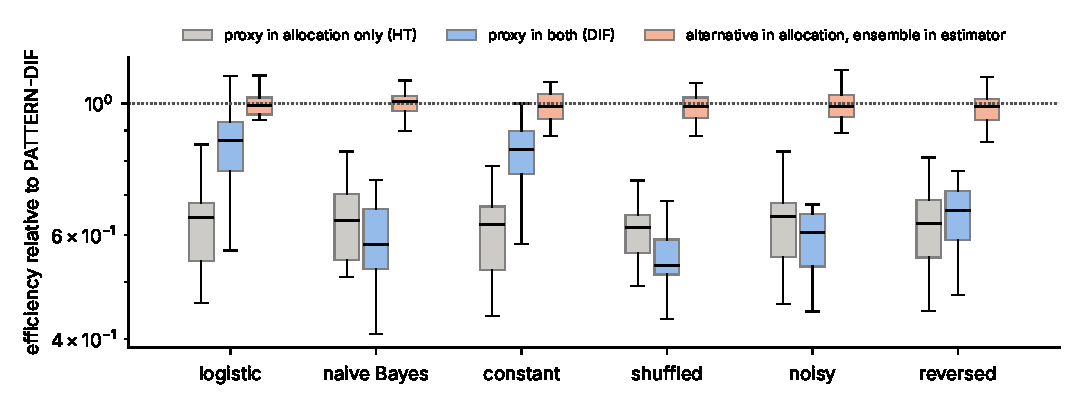
\includegraphics[width=0.95\textwidth]{abl_dif_proxy}
\caption{Efficiency of alternative proxies relative to PATTERN-DIF with the ensemble proxy (Rel.), one value per cell (29 cells; boxes: quartiles, whiskers: 1.5 interquartile ranges). Grey: proxy in the allocation only, plain estimator; blue: proxy in allocation and estimator; orange: proxy in the allocation only, difference estimator with the ensemble proxy.}
\label{fig:abl-proxy}
\end{figure*}

\section{Data sets and models}\label{app:data}

All data sets were obtained from OpenML through scikit-learn's \texttt{fetch\_openml} interface. Adult (version 2, 48,842 records; target income above 50K; groups: sex, female versus male, and race, non-White versus White); Bank Marketing (version 1, 45,211 records; target subscription; group: age below 30); default of credit card clients (version 1, 30,000 records; target default; group: sex); law school admission (binarised version, 20,800 records; group: race, non-White versus White); MAGIC gamma telescope (19,020 records); EEG eye state (14,980 records); Phoneme (5,404 records); Spambase (4,601 records); Churn (5,000 records); Electricity (45,312 records, subsampled to 30,000). For the last six the group is the indicator that the first numeric feature exceeds its median, and the feature is removed from the inputs. In all data sets the minority class is the positive class; for Adult, Bank Marketing and credit-card default this coincides with the conventional positive class (income above 50K, subscription, default).

Each data set was split once, stratified by the label, into a training part (60\%) and a pool (40\%), with seed 0. Numeric features were standardised and categorical features one-hot encoded inside each model's pipeline. The nine models are: logistic regression (default, and with inverse regularisation strength 0.01), decision trees of depth 3 and 12, a random forest with 200 trees and minimum leaf size 3, histogram gradient boosting with default settings, 25-nearest neighbours, Gaussian naive Bayes, and a multilayer perceptron with hidden layers of 64 and 32 units and early stopping. Pool predictions, predicted probabilities, group indicators and labels are cached by \texttt{experiments/preference\_validation.py} and used by all experiments.

\end{appendices}
\end{document}
